%                                     MMMMMMMMM        
%                                                                             
%  MMO    MM   MMMMMM  MMMMMMM   MM    MMMMMMMM   MMD   MM  MMMMMMM MMMMMMM   
%  MMM   MMM   MM        MM     ?MMM              MMM$  MM  MM         MM     
%  MMMM 7MMM   MM        MM     MM8M    MMMMMMM   MMMMD MM  MM         MM     
%  MM MMMMMM   MMMMMM    MM    MM  MM             MM MMDMM  MMMMMM     MM     
%  MM  MM MM   MM        MM    MMMMMM             MM  MMMM  MM         MM     
%  MM     MM   MMMMMM    MM   MM    MM            MM   MMM  MMMMMMM    MM
%
%
%            - META-NET Language White Paper | Serbian content -
% 
% ----------------------------------------------------------------------------

\begin{document}

\maketitle

% --------------------------------------------------------------------------
\bsection*{Предговор --- Preface}

\null
\pagestyle{empty} 

\pagenumbering{Roman} 
\setcounter{page}{3}
\pagestyle{scrheadings}

\begin{Parallel}[c]{78mm}{78mm}
\ParallelLText{
\selectlanguage{serbian}
\parindent20pt

Ова бела књига је део серије која промовише знање о језичким технологијама и њиховим могућностима. Намењена је наставницима језика, новинарима, политичарима, језичким заједницама и другима. 

Покривеност језичким технологијама и начин њихове употребе се у Европи разликују од језика до језика. Због тога се разликују и активности које је потребно спровести да би се подржала истраживања и развој, а неопходни кораци зависе од многих фактора, као што су  сложеност језика или величина заједнице која га користи. 

Пројекат МЕТА-НЕТ, мрежа изврсности коју финансира Европска комисија, спровео је анализу текућих језичких ресурса и технологија. Анализа је била усмерена на 23 званична европска језика, као и на друге значајне националне и регионалне језике у Европи. Резултати анализе сугеришу постојање многих значајних празнина у истраживањима за сваки језик.  Детаљнија експертска анализа и процена текуће ситуације за сваки језик помоћи ће да се повећа утицај нових истраживања и умање могући ризици. 

META-НЕТ повезује 54 истраживачка центра из 33 земље (стр. \pageref{metanetmembers}), који сарађују  са заинтересованим странама из сфера предузетништва, државних институција, привреде, истраживачких организација, софтверских компанија, понуђача технологија и европских универзитета. Они  заједно граде технолошку визију кроз развој стратешких истраживачких програма који показују како ће примене језичких технологија попунити постојеће празнине у истраживањима до 2020. године.}

\ParallelRText{
\selectlanguage{english}
This white paper is part of a series that promotes knowledge about language technology and its potential. It addresses journalists, politicians, language communities, educators and others. 
The availability and use of language technology in Europe varies between languages. Consequently, the actions that are required to further support research and development of language technologies also differ. The required actions depend on many factors, such as the complexity of a given language and the size of its community.

META-NET, a Network of Excellence funded by the European Commission, has conducted an  analysis of current language resources and technologies in this white paper series (p.~\pageref{whitepaperseries}). The analysis focuses on the 23 official European languages as well as other important national and regional languages in Europe. The results of this analysis suggest that there are tremendous deficits in technology support and significant research gaps for each language. The given detailed expert analysis and assessment of the current situation will help maximise the impact of future research.

As of November 2011, META-NET consists of 54 research centres in 33 European countries (p.~\pageref{metanetmembers}). META-NET is working with stakeholders from economy (software companies, technology providers and users), government agencies, research organisations, non-governmental organisations, language communities and European universities. Together with these communities, META-NET is creating a common technology vision and strategic research agenda for multilingual Europe 2020.} 
\ParallelPar
\end{Parallel}

% --------------------------------------------------------------------------

\cleardoublepage

\bsection*{Садржај --- Table of Contents}

\tableofcontents

\addtocontents{toc}{\protect\thispagestyle{empty}\protect}
\addtocontents{toc}{{\Large\textsf{\centerline{СРПСКИ ЈЕЗИК У ДИГИТАЛНОМ ДОБУ}}\par}}

% --------------------------------------------------------------------------

\cleardoublepage

\setcounter{page}{1}
\pagenumbering{arabic} 
\pagestyle{scrheadings}

\selectlanguage{serbian}

% --------------------------------------------------------------------------
\ssection[Резиме] {Резиме}
  
\begin{multicols}{2}



\parindent20pt

У последњих 60 година Европа је постала јединствена политичка и економска структура, мада је културно и језички веома разноврсна. То значи да је, од португалског до пољског, од италијанског до исландског, свакодневна комуникација становника Европе, као и комуникација у сфери пословања и политике, нужно суочена са језичким препрекама. Институције Европске уније троше око милијарду евра годишње на одржавање своје политике вишејезичности, тј. на превођење текстова и говорне комуникације. Питање које се поставља јесте да ли је толико оптерећење неопходно. Модерне језичке технологије и лингвистичка истраживања могу значајно да допринесу брисању језичких граница. Језичке технологије у комбинацији са интелигентним уређајима и апликацијама могу у будућности да помогну Европљанима да се међусобно споразумевају једноставно и лако и да обављају  послове и кад не говоре истим  језиком. 

\boxtext{Jeзичке технологије граде мостове за европску будућност.}

Главни трговински партнери Србије су земље Европске уније, са уделом од преко 50\% у укупној трговинској размени, при чему је извоз из Србије на тржиште ЕУ ослобођен царине у складу са Споразумом о стабилизацији и придруживању. Али језичке препреке могу да зауставе пословање, посебно за СМП (средња и мала предузећа) која немају финансијских средстава да их превазиђу. Једина (незамислива) алтернатива за вишејезичну Европу била би да један језик почне да доминира и на крају замени све остале језике. 

Један традиционални начин превазилажења језичких баријера јесте учење страних језика. Међутим, без технолошке подршке, савладавање 23 званична језика земаља чланица Европске уније и око 60 других европских језика, за становнике Европе представља непремостиву препреку, баш као и за њену економију, политичке дебате и научни напредак. 

Решење лежи у изградњи кључних потпорних технологија. Оне ће европским актерима понудити огромне предности, не само у оквиру заједничког европског тржишта већ и у трговинским односима са трећим земљама, посебно са привредама које се брзо развијају. Да би се постигао тај циљ и очувала европска културна и језичка разноврсност, неопходно је да се прво спроведе систематска анализа језичких специфичности свих европских језика, као и  текућег стања њихове опремљености језичким технологијама. На тај начин ће језичке технологије послужити као јединствени мост међу европским језицима. 

\boxtext{Језичке технологије као решење за будућност}

Алати за аутоматско превођење и обраду говора који се могу наћи на тржишту још увек не омогућавају остварење овог амбициозног циља. Главни актери на овом пољу су пре свега приватна профитна предузећа из Северне Америке. Још крајем 1970-их Европска унија је препознала суштински значај језичких технологија као покретача европског јединства, и почела је са финансирањем првих истраживачких пројеката као што је био пројекат EUROTRA. У исто време, започели су национални пројекти, који су дали вредне резултате, али нису покренули и заједничку усклађену европску акцију. Насупрот овим појединачним и неповезаним напорима у финансирању, друга вишејезична друштва, као што су Индија (22 званична језика) и Јужна Африка (11 званичних језика)  \cite{Meta1}, недавно су почела дугорочне националне програме језичких истраживања и технолошког развоја. 

Данас се главни актери на подручју језичких технологија ослањају на непрецизне статистичке приступе, који не користе дубље лингвистичке методе и знања. На пример, реченице се аутоматски преводе тако што се нове реченице пореде са хиљадама претходно ,,ручно'' преведених реченица. Квалитет резултата у великој мери зависи од квантитета и квалитета расположивог корпуса узорака. Мада машинско превођење једноставних реченица може да пружи употребљиве резултате у језицима са довољном количином расположивог текстуелног материјала, ове плитке статистичке методе нужно доживљавају неуспех у случају језика са мањим обимом узорака или у случају реченица комплексне структуре.

Европска унија је због тога одлучила да финансира пројекте као што су EuroMatrix и EuroMatrixPlus (од 2006) и iTranslate4 (од 2010) који спроводе основна и примењена истраживања и стварају ресурсе за успостављање језичкотехнолошких решења високог квалитета за све европске језике. Анализа дубљих структурних својстава језика је једини начин да се изграде апликације које дају добре резултате на целом распону европских језика.

Европска истраживања у овој области већ су постигла бројне успехе. На пример, преводилачки сервиси Европске уније користе софтвер отвореног кода за машинско превођење MOSES, који је претежно развијен кроз европске истраживачке пројекте. Пројекат Verbmobil, који је финансирало Министарство образовања и истраживања Немачке (German Ministry of Education and Research - BMBF) у периоду 1993-2000, довело је Немачку за неко време на водећу позицију на подручју истраживања превођења говора. Многе истраживачке и развојне лабораторије смештене у то време у Немачкој (нпр.  IBM и Philips) касније су затворене или премештене. Уместо да надграђује истраживачке резултате, Европа је почела да финансира неповезане истраживачке активности са много мањим коначним утицајем на тржиште. Економска вредност ових раних настојања се може сагледати кроз број новопроистеклих предузећа. Компанија Trados, основана још 1984, продата је 2005. године британском предузећу SDL.

\boxtext{Језичке технологије помажу уједињењу Европе.}

Према увиду у досадашње стање, сви су изгледи да ће ,,хибридне'' језичке технологије које комбинују дубинску обраду са статистичким методама бити у могућности да премосте јаз између свих европских језика, и шире. Како показује ова серија белих књига, постоји драматична разлика у степену припремљености када су у питању језичка решења и стање истраживања међу европским језицима.  Српски језик је један од ,,мањих'' европских језика и потребна су даља истраживања која ће омогућити да ефикасна решења која нуде језичке технологије уђу у свакодневну употребу.

Дугорочни циљ МЕТА-НЕТ-а јесте да уведе језичке технологије високог квалитета за све језике, како би се постигло политичко и економско јединство кроз културну разноврсност. Те технологије ће помоћи да се уклоне постојеће баријере и да се изграде мостови међу европским језицима. Ово захтева од свих заинтересованих учесника – у политици, истраживању, привреди и друштву – да уједине своје напоре за будућност. 

Ова серија белих књига допуњује друге стратешке активности које предузима МЕТА-НЕТ (видети преглед у додатку). Ажурне информације као што су текућа верзија текста МЕТА-НЕТ визије  \cite{Meta1} или стратешки истраживачки план рада (Strategic Research Agenda - SRA) могу се наћи на META-НЕТ веб локацији: \url{http://www.meta-net.eu}.   
    
\end{multicols}

\clearpage

% --------------------------------------------------------------------------

\ssection[Опасност по наше језике и изазови пред језичким технологијама] {Опасност по наше језике\newline и изазови пред језичким\newline технологијама}
  
\begin{multicols}{2}

\parindent20pt

Сведоци смо дигиталне револуције која драматично утиче на комуникацију и друштво. Најновија достигнућа на подручју дигиталних информационих и комуникационих технологија могу да се пореде са Гутенберговим изумом штампарске пресе. Шта ова аналогија може да нам каже о будућности европског информационог друштва и посебно наших језика?

\boxtext{Сведоци смо дигиталне револуције која се може упоредити са Гутенберговим изумом штампарске пресе.}

После Гутенберговог изума, стварне продоре у комуникацији и размени знања остварила су дела као што је био Лутеров превод Библије. Током наредних векова у култури су развијене технике за бољу обраду језика и размену знања:

\begin{itemize}
 \item правописна и граматичка стандардизација већих језика омогућила је брзо преношење нових научних и интелектуалних идеја;
 \item развој званичних језика омогућио је становницима да међусобно комуницирају унутар (често политичких) граница;
 \item подучавање и превођење језика омогућило је комуникацију која превазилази језичке границе;
 \item стварање уредничких и библиографских упутстава обезбедило је квалитет и расположивост штампаног материјала;
 \item појавом различитих медија, као што су новине, радио, телевизија, књиге и други облици, задовољене су различите  потребе за комуникацијом. 
\end{itemize}

У последњих двадесет година информационе технологије помогле су да се аутоматизују и поједноставе бројни процеси:

\begin{itemize}
\item софтвер за стоно издаваштво је заменио писаћу машину и слагање текста;
\item Microsoft PowerPoint је заменио графоскопске фолије;
\item документа се шаљу и примају електронском поштом често брже него факс машином;
\item Skype се користи за јефтино телефонирање преко интернета и организовање виртуелних састанака;
\item формати аудио и видео записа олакшавају размену мултимедијалних садржаја;
\item претраживачке машине обезбеђују приступ веб странама преко кључних речи;
\item \textit{онлајн} услуге као што је Google Translate производе брз и  приближни превод;
\item друштвени медији као што су Facebook, Twitter, и Google+ поједостављују  комуникацију, сарадњу и размену информација.
\end{itemize}

Мада су сви ови алати и апликације од велике помоћи, они још нису довољни да остваре одрживо вишејезично европско друштво у коме је свакоме могућ слободан приступ информацијама и роби.
 
% --------------------------------------------------------------------------
\subsection {Језичке границе представљају сметњу за европско информационо друштво}
  
Не можемо тачно да предвидимо како ће изгледати будуће информационо друштво. Али постоје велики изгледи да ће револуција у комуникационој технологији повезати на нове начине људе који говоре различитим језицима. То ствара притисак на појединце да уче нове језике и посебно на развојне тимове да стварају нове технолошке производе који ће обезбедити узајамно разумевање и приступ заједничком знању. У глобалном привредном и информационом простору, нови типови медија омогућавају бржу размену у којој учествују бројни језици, говорници и садржаји. Актуелна популарност друштвених медија као што је Википедија (Wikipedia), Фејсбук (Facebook), Твитер (Twitter), Јутјуб (YouTube) и, однедавно, Гугл+ (Google+) само је  врх леденог брега. 

\boxtext{Глобална економија и глобални информациони простор суочавају нас са различитим језицима, говорницима и садржајима.}

Данас можемо да допремимо гигабајте текста из целог света за свега неколико секунди, пре него што схватимо да је текст на језику који не разумемо. Према недавном извештају Европске комисије, 57\% корисника интернета наручује робу и услуге на језицима који им нису матерњи. (Енглески је најчешћи страни језик а за њим следе француски, немачки и шпански.) 55\% корисника чита садржаје на страном језику, док само 35\% користи страни језик за писање електронских порука или коментара на мрежи  \cite{EC1}. До пре неколико година енглески језик је био lingua franca веба -- огромна већина садржаја на вебу била је на енглеском језику.  Ситуација је данас драстично промењена. Количина онлајн садржаја и на другим европским (као и азијским и средњоисточним) језицима доживела је праву експлозију. 

Ова свеприсутна дигитална подељеност као последица језичких граница изазвала је изненађујуће мало пажње у јавности. Ипак, она поставља неодложно питање: ,,Који ће европски језици напредовати и опстати у умреженом друштву информација и знања, а који су осуђени да нестану?''
 
% --------------------------------------------------------------------------
\subsection {Наши језици су угрожени}
  
Проналазак штампарске пресе допринео је повећању обима размене информација у Европи, али је такође довео до изумирања многих европских језика. На регионалним језицима и језицима мањина ретко се штампало. Ово је довело до тога да су многи језици, као што су корнвалски или далматски, сведени на усмене облике преношења, што је довело до тога да су се све мање користили.  Да ли ће интернет довести до истих последица када су наши језици у питању?

\boxtext{Велика разноврсност језика у Европи јесте једно од њених најдрагоценијих и најзначајнијих културних добара.}

Око 80 језика Европе представља једно од њених најбогатијих и најважнијих културних добара и суштински чинилац њеног друштвеног модела  \cite{EC2}. Док ће језици као што су енглески или шпански вероватно преживети на дигиталном тржишту у настајању, многи би европски језици могли да постану небитни у умреженом друштву. Овакав развој ствари ослабио би позицију Европе у свету, а то би било и у супротности са стратешким циљем да се обезбеди подједнако учешће за сваког становника Европе без обзира на језик. Према УНЕСКО-вом извештају о вишејезичности, језици су суштински медијум за уживање основних људских права као што су изражавање политичких опредељења, образовање и учествовање у друштву  \cite{Unesco1}.


% --------------------------------------------------------------------------
\subsection {Језичке технологије су кључне потпорне технологије}
  
У прошлости, инвестиције у очување језика усмераване су на учење и превођење језика. Према неким проценама, европско тржиште превода, усменог превођења, локализације софтвера и глобализације страница на вебу  2008. год. је износило 8,4 милијарде евра, са очекиваним растом од 10\% годишње \cite{EC3}. Тај износ покрива само мањи део садашњих и будућих потреба у међујезичкој комуникацији. Најубедљивије решење које ће обезбедити дубину и ширину коришћења језика у Европи сутрашњице јесте коришћење одговарајуће технологије на исти начин на који се користе технологије за потребе транспорта, у енергетици или за особе са посебним потребама. 

Дигиталне језичке технологије (којима је циљ да овладају свим облицима писаног и говорног језика) помажу људима да сарађују, послују, размењују знање и учествују у политичким и друштвеним дебатама без обзира на језичке баријере или њихове информатичке вештине. Технологије су често невидљиве у сложеним софтверским системима који нам помажу да:

\begin{itemize}
\item нађемо информацију помоћу претраживачких машина;
\item користимо правописне и граматичке провере у програмима за о\-бра\-ду текста;
\item разгледамо препоруке о производима у мрежним продавницама;
\item саслушамо гласовна упутства у навигационим системима аутомобила;
\item преводимо веб странице помоћу мрежних преводилаца.
\end{itemize}

Језичке технологије чине већи број основних апликација које омогућавају обраду језика у оквирима ширих програмских система. Сврха белих књига, састављених у оквиру МЕТА-НЕТ-а, јесте да се опише степен развоја основних језичких технологија за сваки од европских језика. 

\boxtext{Европи су потребне робусне и приступачне језичке технологије за све европске језике.} 

Да би одржала свој положај у првим редовима светске иновативности, Европи ће бити потребне језичке технологије прилагођене свим европским језицима које ће бити робусне, свима приступачне и потпуно интегрисане у кључна софтверска решења. Без језичких технологија нећемо бити у стању да у скорој будућности остваримо одиста ефикасно интерактивно, мултимедијално и вишејезично корисничко искуство.

% --------------------------------------------------------------------------
\subsection {Могућности језичких технологија}
  

У свету штампане речи, брзо умножавање слике текста (стране) коришћењем штампарске пресе пред\-став\-ља\-ло је технолошки пробој. Људима је био препуштен тешки посао прегледања, читања, превођења и апстраховања знања. Требало је да дочекамо Едисона да бисмо снимили говорни језик, при чему је његова технологија производила само аналогне копије.

Дигиталне језичке технологије данас могу да аутоматизују сам процес превођења, генерисање садржаја и управљање знањем за све европске језике. С њима је могуће опремити кориснику блиске, текстуалне или говорне, сумеђе (интерфејс) за кућне електричне апарате,  машине, возила, рачунаре и роботе. Иако достигнућа истраживања и развоја омогућавају да се наслуте широке могућности, комерцијалне и индустријске примене су још у раној фази развоја. На пример, за многе европске језике машинско превођење достиже задовољавајући ниво тачности у оквиру специфичних домена, а експерименталне апликације обезбеђују вишејезичне информације, управљање знањем и генерисање садржаја. 

Као што је то случај са већином технологија, прве језичке апликације, као што су гласовне корисничке сумеђе и дијалошки системи, развијене су за уско специјализоване домене, а њихова употребљивост је била често ограничена. Међутим, у образовној индустрији и индустрији забаве леже огромне тржишне могућности за интеграцију језичких технологија у игре, странице везане за културно наслеђе, производе за образовање кроз забаву, библиотеке, симулациона окружења или програме обуке. Мобилне информационе услуге, софтвер за рачунарски потпомогнуто учење језика, окружења за електронско учење, алати за самооцењивање и откривање плагијата само су неки од примера где језичке технологије могу да одиграју важну улогу. Популарност друштвених мрежа као што су Твитер (Twitter) и Фејсбук (Facebook) указује да постоје потребе за језичким технологијама које омогућавају надгледање поште, резимирање дискусија, детекцију трендова у испољеним ставовима, препознавање емотивних реакција, идентификацију повреда ауторских права или праћење злоупотреба.

\boxtext{Језичке технологије помажу да се превазиђе ,,хендикеп'' језичке разноликости. }

Језичке технологије представљају огромну прилику за Европску унију. Оне могу да помогну у решавању комплексног питања вишејезичности у Европи -- чињенице да различити језици природно коегзистирају у европском пословању, организацијама и школама. Али грађани желе да комуницирају изван језичких граница које још увек постоје на јединственом европском тржишту. Језичке технологије могу да помогну у превазилажењу ове последње препреке својом подршком слободном и отвореном коришћењу појединачних језика. Ако гледамо и корак даље, иновативне европске вишејезичне технологије представљаће узор за наше партнере по свету када они буду почели да обезбеђују ове технологије за своје вишејезичне заједнице. Језичке технологије могу се посматрати као облик ,,потпорних'' технологија које помажу да се превазиђе ,,хендикеп'' језичке разноликости и да језичке заједнице постану блискије.

Најзад, jедно активно истраживачко подручје  јесте коришћење језичких технологија у операцијама спасавања у областима погођеним  катастрофама, где успешно деловање може одлучивати о животу или смрти: будући интелигентни роботи са вишејезичним способностима у могућности су да спасу животе. 


% --------------------------------------------------------------------------
\subsection{Изазови пред језичким технологијама}
  
Мада су језичке технологије последњих неколико година оствариле значајан напредак, текући темпо технолошког напретка и иновације про\-из\-во\-да је сувише спор. Језичке технологије које су у широкој употреби, као што су граматичке и правописне провере, по правилу су једнојезичне, и постоје само за мали број језика. Онлајн услуге машинског превођења, мада су корисне да се брзо произведе при\-хват\-љи\-ва апроксимација садржаја документа, стварају пуно потешкоћа када је потребно да се произведу високо прецизни и потпуни преводи. Због комплексности природног језика, његово софтверско моделирање и тестирање у реалном свету је дуг и скуп посао, који захтева дугорочно финансирање. Европа мора да одржи своју пионирску улогу у суочавању са технолошким изазовима вишејезичне заједнице изналажењем нових метода којима ће убрзати развој на целој својој територији. У њих би спадале и иновације у области рачунарства и  технике које користе потенцијале великог броја учесника (crowdsourcing). 

\boxtext{Текући темпо технолошког напретка  сувише је спор.}
% --------------------------------------------------------------------------
\subsection {Усвајање језика код људи и машина}
  
Да бисмо илустровали начин на који рачунари поступају са језиком и зашто их је тако тешко испрограмирати да употребљавају језик, бацимо поглед на начин како људи усвајају матерњи и страни језик, а онда погледајмо и како ради језичкотехнолошки систем. 

Људи стичу језичке вештине на два различита начина. Бебе уче језик слушајући  разговоре између родитеља, браће и сестара и других чланова породице. У узрасту од приближно две године деца изговарају своје прве речи или кратке фразе. То је могуће само захваљујући посебној генетској предиспозицији људи да опонашају, а потом и осмисле оно што чују. 

Учење страног језика у старијем узрасту захтева више напора, углавном зато што дете не припада језичкој заједници оних којима је тај језик матерњи. У школи страни језици се обично усвајају учењем граматичких структура, речника и правописа кроз вежбања која описују језичко знање преко апстрактних правила, табела и примера.  Учење страног језика са годинама постаје све теже. 

\boxtext{Људи стичу језичке вештине на два различита начина: учењем примера и учењем језичких правила.}

Два главна типа система језичких технологија „усвајају“ језичке способности на сличан начин као људи. Статистички приступи  (или „приступи вођени подацима“) стичу језичко знање из огромних колекција конкретних примера текстова. За обучавање система за проверу правописа, на пример, довољно је коришћење текстова на једном језику, али су за обучавање машинских преводилаца потребни тзв. паралелни текстови на два (или више) језика. Алгоритам машинског учења затим „учи“ обрасце превођења речи, кратких фраза и комплетних реченица. 

Статистички приступи могу да захтевају милионе реченица јер квалитет резултата расте са порастом броја анализираних текстова. То је један од разлога што добављачи претраживачких машина жељно прикупљају што је могуће више писаног материјала. Исправка правописних грешака у програмима за обраду текста и сервиси као што су Google Search и  Google Translate, ослањају се на статистички приступ. Велика предност статистике је у томе што машина учи брзо по\-нав\-ља\-ју\-ћи циклусе обуке, мада квалитет може да варира на непредвидљив начин. 

Други приступ језичким технологијама, а посебно машинском превођењу, јесте изградња система заснованих на правилима. Експерти из лингвистике, рачунарске лингвистике и рачунарства морају најпре да граматичку анализу изразе кроз систем правила и да саставе листе речи (лексиконе). То је посао који захтева много времена и велики труд. Неки од водећих система машинског превођења заснованих на правилима у сталном су развоју већ више од двадесет година. Предност система заснованих на правилима је у томе што експерти могу детаљније да контролишу обраду језика. То омогућује да се грешке у софтверу систематски поправљају, а кориснику пруже детаљне повратне информације, пре свега када се такви системи користе за учење језика. Због великих трошкова, језичке технологије засноване на правилима до сада су биле развијане само за велике језике.  

Како предности и слабости статистичких система и система заснованих на правилима теже да се допуњују, текућа истраживања усмерена су на хибридне приступе који комбинују те две методологије. Па ипак, ови приступи су до сада били мање успешни у индустријским применама него у лабораторији. 

Као што смо видели у овом одељку, многе апликације које су у широкој употреби у данашњем информационом друштву ослањају се у великој мери на језичке технологије. С обзиром на вишејезичност европске заједнице, ово се посебно односи на њен привредни и информациони простор. Мада су језичке технологије значајно напредовале последњих неколико година, још увек постоје огромне могућности за побољшање квалитета језичкотехнолошких система. У следећем одељку описаћемо улогу српског језика у европском информационом друштву и даћемо оцену текућег стања језичких технологија за српски језик. 

\end{multicols}

\clearpage

% --------------------------------------------------------------------------
\ssection[Српски  језик у европском информационом друштву] {Српски  језик у европском\newline информационом друштву}
\begin{multicols}{2}

\parindent20pt

\subsection{Општи подаци}


Српски стандардни језик је национални стандардни језик Срба и званични језик у Републици Србији. Формиран је на основици млађих екавских и ијекавских штокавских јужнословенских дијалеката у форми коју му је одредио реформатор писаног језика код Срба Вук Караџић (1787-1864), који је истовремено реформисао и ћирилички алфабет и правопис. У 20. веку,  у заједничкој држави Југославији тај језик је обухваћен називом српскохрватски који је имплицирао језичко заједништво са Хрватима (касније и другим народима чији је стандардни језик базиран на штокавским дијалектима). У последњој деценији 20. века уместо назива српскохрватски у Србији је у општој употреби  назив српски језик. Устав Републике Србије из 2006. прописује: ,,Српски језик и ћирилично писмо биће у званичној употреби у Републици Србији'' \cite{Ustav}.

Према попису становништва из 2002, Србија има 7 498 001 становник \cite{VJN3}, а српски је матерњи језик за 88,3\% становништва \cite{HDR}. Томе треба додати и становништво српске националности у другим крајевима бивше Југославије (чији  број није лако одредити). Српска дијаспора, већином настала одласком на рад у иностранство и исељавањем због економских разлога, живи пре свега у појединим земљама централне и западне Европе, у САД, Канади и Аустралији (степен знања српског језика највише је у\-сло\-вљен тиме о којој се генерацији исељеника ради). Према попису из 2002, већина Срба ван земље живи у Немачкој (102 799), затим у Аустрији (87 844) и Швајцарској (65 751). 

\boxtext{Стандардни српски језик је стандардни национални језик Срба и званични језик у Републици Србији.}

Србија је вишејезична заједница. Према попису из 2002, националне мањине \cite{Ombudsman} су Мађари (3,91\%), Бошњаци (2,1\%), Роми (1,44\%), Хрвати (0,94\%), Црногорци (0,92\%), Албанци (0,82\%), Словаци (0,79\%), Југословени (1,08\%) као и друге мањине (Ашкалије, Бугари, Буњевци, Цинцари, Чеси, Горанци, Јевреји, Македонци, Немци, Муслимани, Румуни, Русини, Словенци, Турци, Украјинци и Власи, 2,45\%).  Структура мањинског становништва према језику је следећа: 3,8\% мађарски, 1,8\% бошњачки, 1,1\% ромски, 0,8\% албански, 0,8\% словачки, 0,7\% влашки, 0,5\% румунски, 0,4\% хрватски, 0,2\% бугарски и 0,2\% македонски. Остале језике говори 0,5\% становника, док за 0,8\% становника ови подаци нису познати. За неке мањинске језике у Србији постоји основно и средње образовање, и то за албански (55 основних/4 средње школе), мађарски (108/38), бугарски(26/-), румунски (27/2), русински (3/2), словачки (15/2), хрватски (7/1) \cite{GOD2010}. Настава је праћена и издавањем уџбеника и лектире (нпр. у 2005. издато је укупно 526 уџбеника за основну и 283 за средњу  школу) \cite{HDR}.  Службена употреба језика мањина је уређена законом о службеној употреби језика и писама \cite{SGRS}, који обезбеђује да се закони и прописи објављују на језицима националних мањина. Ово укључује право обраћања републичким органима на свом језику и право да се добије одговор на том језику (у зависности од величине мањинске заједнице). 
Превођење на српски или са српског је значајна активност. Током 2010. године је преведено 2549 дела (са енглеског 1438, са француског 215, са немачког 170, са италијанског 191, са шпанског 74, са мађарског 149). Део превода је са словенских језика (са руског 225, са чешког 4, са пољског 13, са словачког 21, са словеначког 19, са македонског 18, са бугарског 12). Што се тиче превода са српског на друге језике, у Србији је током 2010. објављен 591 наслов.

% --------------------------------------------------------------------------
\subsection {Специфичности српског језика}
  
Српски језик има своје специфичности, које чине његову рачунарску обраду комплексним задатком. 


% --------------------------------------------------------------------------
\subsubsection {Фонетика, фонологија, морфофонологија}
  
Вокалски систем је једноставан (5 вокала), а консонантски релативно комплексан (25 консонаната). Вибрант \textit{р} се у одређеним позицијама изговара као вокал и функционише као носилац слога (силабем), нпр. у речима \textit{п\textbf{р}ст} или \textit{в\textbf{р}ста}. У промени речи и творби речи постоји велики број фонемских алтернација (консонантских, вокалских и комбинованих) које се у неким случајевима комбинују на такав начин да два облика једне речи могу бити веома удаљена, нпр. номинатив сингулара именице „мисао“ је \textit{мисао}, а инструментал сингулара \textit{мишљу} (алтернације \textit{a/\o{}, o/л, л+j/љ/ с/ш}).

Акценатски систем од 4 акцента заснован је на два укрштена параметра: опозиција по дужини  (кратки : дуги) и по тону (силазни : узлазни).  Дистрибуција узлазних и силазних акцената је регулисана посебним правилима. У промени и у творби речи честе су акценатске алтернације. Пошто се акценатски знаци не бележе, у писаном тексту се јављају хомографи. На пример, значење речи \textit{лук} се разликује према томе да ли је акценат краткосилазни или дугосилазни.

У доста речи и граматичких облика кодификована норма предвиђа изговор постакценатских дужина, али се оне у узусу све мање изговарају.

Скоро све речи су наглашене, али постоје и клитике: проклитике (већина везника и предлога, као и негација уз глагол) и енклитике (ненаглашени облици заменица и глагола и упитна партикула \textit{ли}).

Изговор позајмљеница је фонетски прилагођен српском језику. Комбинације фонема (пре свега консонаната) у позајмљеницама често одступају од група које су типичне за изворне штокавске речи, као у примерима \textit{со\textbf{фтв}ер}, \textit{ха\textbf{рдв}ер}, \textit{интерфе\textbf{јс}}. Има такође, нарочито у свакодневном узусу, одступања и од нормативне дис\-три\-бу\-ци\-је акцената.

Код једног броја лексема и облика постоје две варијанте изговора - екавска и ијекавска - етимолошки везане за некадашњи вокал звани \textit{јат}, као што је показано у табели \ref{ekavski_ijekavski}. 

\arrayrulecolor{white}

\begin{table*}[ht]
\begin{center}
\renewcommand{\arraystretch}{2.2}
\setlength{\arrayrulewidth}{1pt} 
\begin{tabular}{|>{\columncolor{orange1}}c|>{\columncolor{orange1}}c|>{\columncolor{corange2}}c|>{\columncolor{corange2}}c|}
 \hline
  %\rowcolor{orange1}
  \multicolumn{2}{|>{\columncolor{orange1}}c|}{} & \cellcolor{orange1}\textcolor{white}{\textbf{екавски}} & \cellcolor{orange1}\textcolor{white}{\textbf{ијекавски}} \\ 
   \hline
  \textcolor{white}{,,цвет''} & \textcolor{white}{сингулар} & \textit{цв\textbf{е}т} (дуго \textbf{е}) & \textit{цв\textbf{ије}т}\\ 
   \cline{2-4}
     & \textcolor{white}{плурал} & \textit{цв\textbf{е}тови} (кратко \textbf{е}) & \textit{цв\textbf{је}тови} \\
  \hline
 \end{tabular}
\end{center}
\caption{Екавска и ијекавска варијанта изговора}
\label{ekavski_ijekavski}
\end{table*}

% --------------------------------------------------------------------------
\subsubsection {Морфологија (врсте, промена и творба речи)}
  
Постоји десет врста речи, са великим бројем подврста. Посебно су комплексни системи заменица и бројева. Не постоји члан.

Именице имају род као класификациону категорију (мушки, женски или средњи). Од значаја је и класификација према семантичком роду (мушки или женски). На пример, именица \textit{газда} се мења као именица женског рода, али означава мушку особу. 

Глаголи имају вид као класификациону категорију (свршени или  несвршени). Известан број глагола има оба вида. Постоји више врста такозваних рефлексивних глагола. 

Постоје три типа флексије: (а) деклинација (по броју и падежу код именица (видети табелу \ref{imenicke_fleksije}), по роду, броју, падежу и придевском виду код придева); (б) конјугација (веома комплексна); и (в) компарација (код градабилних придева и прилога).  Све промене имају мањи или већи број ужих типова, као и известан број изузетака. Свуда постоје бројне фонемске и акценатске алтернације. Посебно треба истаћи велики број подударних облика, тј. облички синкретизам (морфолошку хомонимију). Последица флексије је да речнику од 120.000 лема одговара око 4,5 милиона флективних граматичких облика (ипак нема толико формалних речи јер су неки облици у појединим парадигмама истоветни). 

\begin{table*}[ht]
\begin{center}
\renewcommand{\arraystretch}{2.2}
\setlength{\arrayrulewidth}{1pt}
\begin{tabular}{|>{\columncolor{orange1}}c|>{\columncolor{corange1}}c|>{\columncolor{corange1}}c|>{\columncolor{corange1}}c|}
\hline
\rowcolor{orange1}
\textcolor{white}{\textbf{4 типа именичке флексије}} & \textcolor{white}{\textbf{сингулар}} & \textcolor{white}{\textbf{паукал (2-4)}} & \textcolor{white}{\textbf{плурал}} \\
\hline
\textcolor{white}{\textbf{,,прозор'' (м. род)}} & \textit{прозор} & \textit{прозор\textbf{а}} & \textit{прозор\textbf{и}} \\
\hline
\textcolor{white}{\textbf{,,jaje'' (с. род)}} & \textit{jaj\textbf{e}} & \textit{јајет\textbf{а}} & \textit{jaj\textbf{a}} \\
\hline
\textcolor{white}{\textbf{,,жена'' (ж. род)}} & \textit{жен\textbf{а}} & \multicolumn{2}{>{\columncolor{corange1}}c|}{\textit{жен\textbf{е}}} \\
\hline
\textcolor{white}{\textbf{,,вест'' (ж. род)}} & \textit{вест} &  \multicolumn{2}{>{\columncolor{corange1}}c|}{\textit{вест\textbf{и}}} \\
\hline
\end{tabular}
\end{center}
\caption{4 типа именичке флексије}
\label{imenicke_fleksije}
\end{table*}


Личне заменице (укључујући и рефлексивну заменицу) и помоћни, копулативни и егзистенцијални глагол „јесам“ и помоћни глаголи „бити“ и „хтети“ имају и енклитичке облике, који се чешће користе од одговарајућих наглашених облика. На пример, датив једнине мушког и средњег рода личне заменице трећег лица гласи: \textit{њему} (акцентовани облик) и \textit{му} (енклитички облик).

Код именица, глагола и придева постоји веома развијена суфиксална творба речи. Код глагола је веома развијена и префиксација (добрим делом повезана и са аспекатским значењима). Композиција, у целини гледано, мање је развијена. 

Постоји пуристички однос према калковима и кованицама, као и према тзв. есоцентричним именичким сложеницама, као нечем што не спада у аутентичну  штокавску творбу. Овакав однос отежава лексичку и терминолошку елаборацију коришћењем творбе речи и један је од разлога веома великог броја позајмљеница.

Позајмљенице се већином уклапају у постојеће морфолошке и творбене типове, али од тога има одступања. На пример, неке стране речи се не мењају, као што су именице \textit{Мери} и \textit{скво} или придеви \textit{фер} или \textit{браон}. 

Развијена творба речи (суфиксација, префиксација, у мањој мери композиција и разни комбиновани творбени начини) чине да се највећи број лексема може груписати у творбене породице односно лексикографска гнезда. Ту је посебно важно да један део творбених веза доводи до систематске (категоријалне) модификације значења основне речи,  што знатно олакшава лексикографску обраду таквих случајева. На пример, за реч ,,глумац'' твори се деминутив ,,глумчић'' и аугментатив ,,глумчина'', женски облик ,,глумица'' и придеви ,,глумчев'', ,,глумичин'', ,,глумачки'', итд. 

Позајмљенице су у принципу фонолошки и морфолошки адаптиране, тј. прилагођене изговору и морфологији српског језика. И од њих се образују творбене породице.


% --------------------------------------------------------------------------
\subsubsection {Лексика, фразеологија, терминологија, ономастика}
  
Састав лексике одражава, с једне стране,  штокавску основицу, и то не само у погледу оригиналног инвентара него и у погледу нових речи творених према новоштокавским творбеним моделима. С друге стране, фонд лексема одражава и језичку и културну историју српског народа, укључујући позајмљенице из црквенословенског, турског (,,мегдан''), руског (,,запета''), немачког (,,штрудла''), француског (,,руж'') и, поготову у данашње време, енглеског (,,паркинг''). Томе треба додати, поготову у стручним терминологијама, интернационализме засноване на класичним језицима (грчком и латинском).

У области фразеологије посебно треба споменути идиоматске изразе, сликовита поређења, изреке и сл. који одражавају аутохтону имагинацију и језичку креативност. С друге стране, велики број лексикализованих израза је настао и настаје и даље калкирањем  страних израза, данас пре свега енглеских.

Терминологија (и номенклатура) добрим делом се ослањала и ослања се и даље на поједине стране терминологије, путем превођења или позајмљивања (нарочито кад су у питању терминолошки интернационализми).  Напори да се нађу изворна српска решења или да се постојећи термини посрбе имају одређене резултате, али не могу да иду у корак са све већим потребама у области терминологије и номенклатуре.  

Ономастика представља важан део вокабулара српског језика, утолико више што се и овде стварају творбене породице речи.


% --------------------------------------------------------------------------
\subsubsection {Синтакса, лингвистика текста}
  
Што се тиче распореда реченичних конституената (субјекта, предиката, објекта итд.), српски језик спада у тзв. SVO језике са слободним редом речи (тачније речено: са слободним распоређивањем реченичних конституената). То значи да су у принципу све пермутације реченичних конституената дозвољене, а да је преферентни распоред: субјекат - предикат - објекат. Међутим, слободан не значи и анархичан; напротив, избор конкретног распореда је регулисан комбинацијама различитих синтаксичких, семантичких, прагматичких и стилских фактора, тј. ма колико разноврсни, распореди чине један веома комплексан функционални систем. Погледајмо реченицу на енглеском: 
\begin{itemize}
\item \textit{Mary gave John an apple. [Марија даде Јовану јабуку.]} 
\end{itemize}
У српском се ова ситуација може изразити на 24 = 4! = 1*2*3*4 (број пермутација од четири речи) различитих начина:

\begin{itemize}
 \item \textit{Марија даде Јовану јабуку.}
 \item \textit{Марија даде јабуку Јовану.} 
 \item \textit{Марија Јовану даде јабуку.} 
 \item \textit{Марија јабуку даде Јовану.}
 \item \textit{Јовану даде Марија јабуку.}
 \item \textit{Јовану Марија даде јабуку.}
 \item \textit{Јабуку Марија даде Јовану.}
 \item \textit{Јабуку Јовану даде Марија.}
 \item \textit{Даде Марија јабуку Јовану.} 
 \item \textit{Даде Јовану јабуку Марија,} итд.
\end{itemize}
Поједини конституенти се исказују и енклитикама, које се распоређују на сасвим специфичан начин.

Заменички субјекат се не мора исказати, него се може само подразумевати (тзв. нулти субјекат), као у примеру \textit{\textbf{Ja} се зовем Марко} према \textit{Зовем се Марко}. Значајан број реченичних образаца је формиран са разним типовима семантичких субјеката.

Поред актива и пасива, постоји и специјалан начин формулисања реченице са неспецификованим хуманим агенсом, коришћењем облика повратног глагола.

Негација се примењује и на глагол и на заменички конституент (тзв. двострука негација), нпр. \textit{Овде \textbf{не} познајем \textbf{никог}}.

У српском постоји седам падежа: номинатив, генитив, датив, акузатив, вокатив, инструментал и локатив (видети табелу \ref{imenicka_deklinacija}). 

\begin{table*}[ht]
\begin{center}
\setlength{\arrayrulewidth}{1pt}
\renewcommand{\arraystretch}{2.2}
\begin{tabular}{|>{\columncolor{orange1}}c|>{\columncolor{corange1}}c|>{\columncolor{corange1}}c|>{\columncolor{corange1}}c|}
\hline
\rowcolor{orange1} \textcolor{white}{\textbf{Пример именичке деклинације}} & \textcolor{white}{\textbf{сингулар}} & \textcolor{white}{\textbf{паукал}} & \textcolor{white}{\textbf{плурал}} \\
\hline
\textcolor{white}{\textbf{Номинатив}} & \textit{прозор} & \textit{прозор\textbf{а}} & \textit{прозор\textbf{и}} \\
\hline
\textcolor{white}{\textbf{Генитив}} & \textit{прозор\textbf{а}} & & \textit{прозор\textbf{а}} \\
\hline
\textcolor{white}{\textbf{Датив}} & \textit{прозор\textbf{у}} & & \textit{прозор\textbf{има}} \\
\hline
\textcolor{white}{\textbf{Акузатив}} & \textit{прозор} & \textit{прозор\textbf{а}} & \textit{прозор\textbf{е}} \\
\hline
\textcolor{white}{\textbf{Вокатив}} & \textit{прозор\textbf{е}} & \textit{прозор\textbf{а}} & \textit{прозор\textbf{и}} \\
\hline
\textcolor{white}{\textbf{Инструментал}} & \textit{прозор\textbf{ом}} & & \textit{прозор\textbf{има}} \\
\hline
\textcolor{white}{\textbf{Локатив}} & \textit{прозор\textbf{у}} & & \textit{прозор\textbf{има}} \\
\hline
\end{tabular}
\end{center}
\caption{Пример именичке деклинације}
\label{imenicka_deklinacija}
\end{table*}

У српском језику постоји пет зависних падежа, који се сви комбинују и са предлозима. Сви ти падежи и предлошко-падежне комбинације су полисемични. И обрнуто, исто значење се у неким случајевима може исказати различитим падежима односно предлошко-падежним конструкцијама (падежна синонимија). Постоји такође и један број израза који имају функцију предлога, на пример, \textit{приликом} (+генитив).

У српском језику постоји развијен систем личних глаголских облика за исказивање временских и модалних значења (аспекат је класификациона категорија); сви ти облици су полисемични. Једна од специфичности глаголског система је да конструкција \textit{да} + презент све више истискује инфинитив.

Конгруенција у роду, броју, падежу и лицу је један од битних аспеката синтаксе српског језика, а значајна је и за успостављање текстуалних веза. Категоризација контролора конгруенције (нарочито појединих типова именица, конструкција са бројевима и координативних  израза), као и начини на које се та контрола испољава у разним конгруентним позицијама представља и\-зу\-зе\-тно комплексно подручје.

Већина типова зависних реченица (нарочито односне, временске, условне и узрочне) имају више формалних и семантичких подтипова. 

Код координативних реченица посебно је комплексан инвентар везника за копулативне и за адверзативне односе.

Везе међу исказима у тексту се успостављају текстуалним координаторима и текстуалним конекторима разних врста. Избор распореда реченичних конституената важан је за информативну кохеренцију и прогресију, с једне, а за емфазу и истицање, с друге стране. Тзв. нулти субјекат и енклитички заменички облици су важна средства за контекстуализацију реченица.


% --------------------------------------------------------------------------
\subsubsection {Правопис (алфабет, тип правописа, интерпункција, писање страних речи)}
  
Традиционални српски алфабет је ћирилица, коју чини 30 графема. Данас се користи - све више - и латиница. Она такође има 30 графема (три од њих су диграми), који су у бијективном односу са ћириличким графемама. Међутим, званично писмо је само ћирилица (видети табелу \ref{azbuka}).

\begin{table*}[ht]
\begin{center}
\renewcommand{\arraystretch}{1.5}
\setlength{\arrayrulewidth}{1pt}
\begin{tabular}{|>{\columncolor{orange1}}c|>{\columncolor{corange1}}c|>{\columncolor{corange1}}c|>{\columncolor{corange1}}c|>{\columncolor{corange1}}c|>{\columncolor{corange1}}c|>{\columncolor{corange1}}c|>{\columncolor{corange1}}c|>{\columncolor{orange2}}c|>{\columncolor{corange1}}c|>{\columncolor{corange1}}c|>{\columncolor{corange1}}c|>{\columncolor{corange1}}c|>{\columncolor{corange1}}c|>{\columncolor{red}}c|>{\columncolor{corange1}}c|}
\arrayrulecolor{white}
\cline{2-16}
\multicolumn{1}{>{\cellcolor{white}}c}{} & \multicolumn{15}{>{\columncolor{orange1}}c|}{\textcolor{white}{\textbf{Српска слова}}} \\
\hline
\textcolor{white}{\textbf{ћирилица}} & А & Б & В & Г & Д & \cellcolor{orange2}Ђ & Е & Ж & З & И & Ј & К & Л & \textcolor{white}{Љ} & М \\ 
         & а & б & в & г & д & \cellcolor{orange2}ђ & е & ж & з & и & ј & к & л & \textcolor{white}{љ} & м \\
\hline
\textcolor{white}{\textbf{латиница}} & A & B & V & G & D & \cellcolor{orange2}Đ & E & Ž & Z & I & J & K & L & \textcolor{white}{Lj} & M \\
         & a & b & v & g & d & \cellcolor{orange2}đ & e & ž & z & i & j & k & l & \textcolor{white}{lj} & m \\
\hline
\textcolor{white}{\textbf{ћирилица}} & Н & \cellcolor{red}\textcolor{white}{Њ} & О & П & Р & С & Т & Ћ & У & Ф & Х & Ц & Ч & \textcolor{white}{Џ} & \cellcolor{orange2}Ш \\
        & н & \cellcolor{red}\textcolor{white}{њ} & о & п & р & с & т & ћ & у & ф & х & ц & ч & \textcolor{white}{џ} & \cellcolor{orange2}ш \\
\hline
\textcolor{white}{\textbf{латиница}} & N & \cellcolor{red}\textcolor{white}{Nj} & O & P & R & S & T & Ć & U & F & H & C & \cellcolor{orange2}Č & \textcolor{white}{Dž} & \cellcolor{orange2}Š \\
         & n & \cellcolor{red}\textcolor{white}{nj} & o & p & r & s & t & ć & u & f & h & c & \cellcolor{orange2}č & \textcolor{white}{dž} & \cellcolor{orange2}š \\
\hline
\end{tabular}
\end{center}
\caption{Српска слова}
 \label{azbuka}
\end{table*}

Што се тиче графије (односа графемског и фонемског система), графеме и фонеме стоје  у бијективном односу.

На нивоу кодних схема, латинични диграфи \textit{lj}, \textit{nj}, \textit{dž} могу бити кодирани као лигатуре или као диграфи. У првом случају, \textit{Unicode} \cite{UNICODE} обезбеђује, на пример, посебно кодове за лигатуре LJ, Lj и lj који су у случају диграфа представљени као комбинација два ASCII кода,  нпр. L и J. Ово води у проблеме са транслитерацијом  која се, у општем случају, може извршити аутоматски. На пример, сваки чланак на српској Википедији се може приказати и ћириличним и латиничним писмом. 

Азбука у српском не предвиђа употребу латиничних карактера q, x, y, w нити латиничних карактера за записивање римских бројева, што може да доведе до деградације информације приликом транслитерације из латинице у ћирилицу. Тако, на пример, \textit{www} може постати \textit{њњњ}, а латинично \textit{Petar II} може постати \textit{Петар ИИ} уместо \textit{Петар II}. 

Оба алфабета се користе у савременој издавачкој продукцији. Према подацима из Народне библиотеке Србије, током 2010. објављене су укупно 12574 књиге. Од тог броја, 6459 је на ћирилици, 6050 на латиници, а 65 на другим алфабетима. Међу дневним листовима са широким кругом читалаца, Политика и Вечерње новости излазе на ћирилици, док је већина других листова (Блиц, Курир, Данас, итд.) на латиници. 

Правопис је (квази)фонемског типа: са малим изузецима, реч се пише онако како се изговара (правило: ,,\textit{Пиши као што говориш!}''), тачније речено, према свом фонемском саставу.

Интерпункција је логичког, а не граматичког типа (слична француској и енглеској).

Према правопису, стране речи се и ћирилицом и латиницом пишу онако како се изговарају, тј. транскрибовано. И страна имена се такође транскрибују (нпр. уместо \textit{Shakespeare} пише се, и изговара, \textit{Шекспир} и \textit{Šekspir}).

% --------------------------------------------------------------------------
\subsubsection {Српски и други стандардни језици штокавског порекла}
  
Заједничка штокавска основица, међусобни утицаји и коегзистенција у оквиру исте државе и - концептуално - у оквиру заједничког српскохрватског језика чине да за рачунарску обраду других језика  штокавске провенијенције (хрватског, бошњачког, црногорског) треба разрешити сличне проблеме. То отвара велике могућности за синергију или бар за продуктивну сарадњу, као и за  рационалан и економичан приступ решавању заједничких проблема. Томе доприноси и постојање знатних језичких ресурса за некадашњи заједнички српскохрватски језик (граматике и речници), у којима, истина, није поклањана дуж\-на пажња диференцијацијама унутар штокавског стандарднојезичког простора. У ствари, овде се не ради о превођењу текстова с једног страног језика на други, него о \textit{адаптирању} текстова састављених на језицима са истом дијалекатском основицом и са тесно повезаним развојем. 

\vspace{-1cm}
\boxtext{Стандардни језици штокавског порекла морају да реше сличне проблеме. То отвара велике могућности за синергију, или бар за продуктивну сарадњу, као и за  рационалан и економичан приступ решавању заједничких проблема. }

Главни проблеми се, у ствари, тичу појава везаних за елаборацију штокавског језгра и, посебно, за терминологију.





% --------------------------------------------------------------------------
\subsection {Савремени развој}
  
Промене крајем двадесетог и почетком двадесет првог века обухватају следеће:
\begin{itemize}
 \item Уместо заједничког српскохрватског стандардног језика, сада званично постоје четири национална стандардна језика. Конкретно, у Србији је сада званични језик српски, а не више српскохрватски. Због недавних сеоба изазваних ратним збивањима делимично је промењена дијалекатска слика у Хрватској и Босни и Херцеговини (у подручјима захваћеним ратним збивањима). 
\item Уочавају се све веће промене у лексици и фразеологији и у терминологији, везане за политичке, друштвене и економске промене у Србији и отварање према свету, али и за усклађивање законодавства, стандарда и терминологије са законодавством, стандардима и терминологијом који важе у Европској унији. Посебно се уочава утицај енглеског језика, и то не само због културолошких и економских момената који важе и за друге европске земље него и зато што се за усклађивање са Европском унијом као изворници узимају текстови/верзије на енглеском језику. 
\item Латиница се све више употребљава (сем у званичним текстовима).
\item Текстови на српском језику се све више реализују у дигиталном облику (употреба рачунара, електронско издаваштво, интернет, SMS-поруке). 
\end{itemize}

% --------------------------------------------------------------------------
\subsection {Неговање језика у Србији}

\subsubsection{Рад на нормирању и неговању језика}   

\boxtext{Стандардизација српског језика институционализована је кроз Одбор за стандардизацију српског језика, међуакадемијско и међууниверзитетско тело. }

 Овде се може навести следеће:
\begin{itemize}
\item Године 1997. створено је међуакадемијско и међууниверзитетско тело под називом \textit{Одбор за стандардизацију српског језика} \cite{BSSL}, у коме су представници одговарајућих институција из Србије, Црне Горе и Републике Српске (у БиХ). 
\item Уместо раније опште српскохрватске норме, сада се спецификује норма српског језика.
\item Нема пуризма у односу на кроатизме (речи преузете из хрватског). 
\item Израђен је правопис српског језика.
\item Подржава се употреба ћирилице, која се сматра угроженом све већом употребом латинице, нарочито код млађих генерација. 
\item Наставни програми и уџбеници у основној и средњој школи усклађени су са новом стандарднојезичком ситуацијом.
\end{itemize}
 
% --------------------------------------------------------------------------
 \subsubsection {Осавремењивање норме}
   
  Одбор за стандардизацију српског језика је организовао израду серије описно-нормативних монографија које треба да прикажу савремено стање језика и понуде нормативна решења (досада су обрађене: творба речи, синтакса и фонологија). Донет је већи број нормативних препорука. Званични правопис је два пута осавремењиван.

% --------------------------------------------------------------------------
 \subsubsection {Неговање језичког узуса}
 
Одбор за стандардизацију српског језика (својим препорукама), Друштво за српски језик и књижевност (публикацијама и организовањем такмичења из српског језика и језичке културе за ученике основних и средњих  школа), Матица српска (организовањем рада на изради правописа, својим публикацијама и организовањем саветовања о језику), Вукова задужбина (својим публикацијама и организовањем трибина и саветовања о језику) и разне друге институције, поједине издавачке куће и редакције дневних листова и редакције радио и ТВ програма, као и језички стручњаци и љубитељи матерњег језика труде се да дају свој допринос чувању правилности и чистоте српског језика у писаној и усменој употреби.  

% --------------------------------------------------------------------------
\subsubsection {Одговор на све већи утицај енглеског језика}
   
 Истиче се потреба за замењивањем енглеских речи и израза српским, као и за замењивањем калкираних преведеница са енглеског (аутентичним) српским речима и изразима. (Шире узев, овде спада и отпор све већој употреби латинице.)
 
% --------------------------------------------------------------------------
 \subsubsection {Побољшање стања у области лексикографије}
   
 Поклања се све већа пажња лексикографији, једнојезичној и двојезичној. Израђен је велики једнотомни речник савременог српског језика, за којим се осећала велика потреба. Модернизује се рад на изради великог академијског речника српског језика.
Преводе се закони и прописи који важе у Европској унији \cite{SEIO}, као и међународни стандарди \cite{ISS}, укључујући терминолошке стандарде.
 
% --------------------------------------------------------------------------
 \subsection {Језик и образовање}
   
 
Предмет \textit{Српски језик и књижевност} је један од битних предмета у основној и средњој  школи. Међутим, настава је концентрисана на правилно писање и говор, знање о језику (о граматици и лексици), знање о историји књижевних (писаних) језика код Срба и о постанку српског стандардног језика. На оваквој настави су базирана и масовна такмичења из матерњег језика (почев од виших разреда основне школе). Недовољно пажње се поклања практичној употреби језика и функционалној писмености. 
Жеља да се настава по својим циљевима и стандардима приближи настави у Европској 
унији, као и   незадовољавајући успеси ученика на PISA тестирању представљају подстицаје за модернизацију наставе језика и за инсистирање на функционалној писмености и комуникационим способностима. То се одражава и на текућу реформу  школства (циљеви наставе језика, стандарди постигнућа, силабуси), као и на побољшање квалитета уџбеника. На факултетима углавном недостају курсеви из српског језика који би систематски оспособљавали будуће стручњаке за успешну професионалну комуникацију и одговарајућу функционалну писменост. 
Примена језичких технологија свакако може допринети  модернизовању наставе, нпр. применом система за рачунарски потпомогнуто учење језика (CALL). 
 
% --------------------------------------------------------------------------
 \subsection {Међународни аспекти}
   
 
Званична употреба и настава српског језика у државама у којима живе делови српског народа регулисана је законодавством тих држава. 
Нестанак заједничког српскохрватског језика и званично постојање посебних језика штокавске провенијенције одразило се на организацију наставе некадашњег српскохрватског језика на иностраним универзитетима, као и на називе факултетских одсека на којима се држала та настава: сада за те језике, дакле и за српски језик (и књижевност), постоје посебни програми и дипломе, са већим или мањим комбиновањем предмета, а одсеци имају збирне називе.
У Србији се наставља пракса организовања летњих  школа за странце, али сада за српски, а не српскохрватски језик. Такође се шаљу домаћи наставници да раде као лектори на катедрама у иностранству. 
За децу српског порекла организује се у појединим земљама додатна настава из матерњег језика. 
Потреба усклађивања законодавства и терминологије са оним у Европској унији, утицај англо-америчке културе у области забаве и медија и ефекти глобализације све јаче доводе српски језик у везу са другим језицима, нарочито енглеским, и дају преводилаштву све већи  подстицај и значај.

% --------------------------------------------------------------------------
 \subsection {Српски језик на интернету}
   
Анкета \cite{PKEY204} извршена 2010. године говори да 50,8\% становништва редовно користи рачунар и интернет, а 43,7\% становништва никада није користило рачунар. Према другом извору \cite{EUROPA2}, чак 55,9\% популације користи интернет, при чему је стопа раста 926,8\% у периоду 2000-2010. Према истом извору, у Србији на дан 31. августа 2010. било је 2,237,680 корисника Фејсбука, што представља 30,5\% укупне популације. Електронске услуге јавне администрације (e-government) користи  свега 13,2\% становништва, док 38,5\% не би никада користило ове услуге. Трговину преко интернета користило је свега 13\% становништва. Према Републичком заводу за статистику Републике Србије \cite{WEBRZS}, коришћење информационо-комуникационе опреме показује раст приказан у табели \ref{stanovnistvo}.

\begin{table*}[ht]
\begin{center}
\renewcommand{\arraystretch}{2.2}
\setlength{\arrayrulewidth}{1pt}
\begin{tabular}{|>{\columncolor{corange1}}c|>{\columncolor{corange1}}c|>{\columncolor{corange1}}c|}
\arrayrulecolor{white}
\hline
\rowcolor{orange1} \textcolor{white}{\textbf{Домаћинства у Србији имају}} & \textcolor{white}{\textbf{2006}} & \textcolor{white}{\textbf{2010}} \\ 
\hline
рачунар & 26,5\% & 50,4\% \\
\hline
лаптоп & 1,5\% & 11,2\% \\
\hline
приступ интернету & 18,5\% & 39\% \\
\hline
кабловску ТВ & 30,2\% & 42,6\% \\
\hline
мобилни телефон & 71,2\% & 82\% \\
\hline
\end{tabular}
\end{center}
\caption{Коришћење информационо-комуникационе опреме у Србији}
\label{stanovnistvo}
\end{table*}

Према истом извору, 96,8\% фирми користило је интернет 2010. године у поређењу са 90,2\% у  2006, док је 67,5\% фирми имало  своју веб локацију 2010. године у поређењу са 52,9\% у 2006. У 2010. години 70,6\% користило је услуге јавне администрације.

Подаци Републичког завода за статистику из истраживања из 2010. на узорку од 2.400 домаћинстава и исто толико појединаца старости од 16 до 74 године показују да интернет прикључак има 39 одсто анкетираних, највише у Београду - 51 одсто \cite{ICT2010}. Да приступ глобалној мрежи не зависи само од техничких могућности него и од зараде, види се из податка да 83\% домаћинстава са месечним приходима вишим од 600 евра има интернет, док га код оних са примањима нижим од 300 евра има 29\% домаћинстава. Највише људи, 91\%, светској мрежи приступа са десктоп рачунара, петина са мобилног телефона, а нешто мање од тога са лаптопа. 

Кад је реч о типу везе, скоро половина домаћинстава у Србији која користе интернет има ADSL прикључак, четвртина кабловски интернет, а мобилне уређаје за повезивање користи 29\% испитаника. Најчешће се приступа од куће (84\%), затим с посла, од куће друге особе, у школи и на факултету, а  тек 3,8\% из интернет кафеа. Најзаступљенија категорија на мрежи су студенти, чак 95\%. Ако није реч о пословним обавезама, интернет се највише користи за електронску пошту – 78\%, затим за забаву (игре, филмови, музика) – 55\%, за читање штампе – 41\% и за учење – 23\%. Најпопуларније српске веб странице су портали са вестима (Блиц \cite{BLIC}, Б92 \cite{B92}, Наслови \cite{NASLOVI} и РТС \cite{RTS}). Најпосећенији домаћи портал је Krstarica \cite{KRSTARICA},  која укључује претраживачку машину, ажурне дневне вести из Србије, каталог локалних страница груписаних по тематици и разноврсне друге садржаје. Експеримент започет 2005.  увођењем локалне претраживачке машине \textit{Pogodak}, која је претрагу прилагођавала морфологији српског, окончан је 2010. као непрофитабилан. 

Википедија на српском представља извор разноврсних језичких података. Она садржи око 142.000 чланака и налази се на  28. месту \cite{WIKI} у свету у погледу броја објављених чланака. Википедија на српскохрватском \cite{SHWIKI}   је мања и  има око 40.000 чланака. Слободан приступ језичким подацима је могућ и преко портала \textit{Растко} \cite{RASTKO},  \textit{Антологија српске књижевности} \cite{ASK} и \textit{Транспоетика} \cite{TRPOET}, који садрже углавном књижевне текстове. 

Видљивост појединих страна са садржајем на српском је привремено драматично пала током 2010. као последица преласка са топ-домена yu на rs. 

Најчешће коришћена веб апликација је претрага веба. Она укључује аутоматску обраду језика на више нивоа, што ће бити детаљније описано у другом делу овог текста.  Оваква обрада укључује префињене језичке технологије које се разликују за сваки језик.  За српски, како је већ поменуто,  проблеми настају због односа између латиничног и ћириличног писма,  екавских и ијекавских варијација, графемских варијација у облику леме, као и морфолошког богатства. 

Користи које корисници интернета и добављачи садржаја на вебу могу да имају од језичких технологија можда су мање очигледне, на пример, у аутоматском превођењу веб садржаја са једног језика на други. Упркос високој цени ручног превођења, релативно мало језичких технологија је развијено и примењено у односу на уочене потребе.  Разлог за то може бити у сложености српског језика и бројним технологијама које је потребно упослити за развој типичне језичке апликације. У следећем одељку представићемо преглед језичких технологија и основне области примене,  као и оцену текуће ситуације у подршци језичким технологијама српског језика.
\end{multicols}

\clearpage

% --------------------------------------------------------------------------
 \ssection[Jезичкe технологијe за српски језик]{Jезичкe технологијe за српски\newline језик}
\begin{multicols}{2}   

\parindent20pt

Језичке технологије су софтверски системи пројектовани за рад са природним језицима. Због тога се ове технологије често подводе под термин „технологија природних језика“. Природни језици се јављају у говорном и писаном облику. Иако је говор најстарији и са становишта човекове еволуције најприроднији начин језичке комуникације, комплексне информације и свеобухватно људско знање се бележе и преносе у писаном облику. Говорне и текстуалне технологије обрађују и производе језик у ова два облика и оба користе речнике и граматичка и семантичка правила. То значи да језичке технологије повезују језик са различитим облицима знања независно од медија (говорних или текстуалних) којима су представљена. Слика \ref{fig:ltincontext_sr} илуструје пејзаж језичких технологија. Када комуницирамо, ми комбинујемо језик са другим начинима комуникације и другим информационим медијима. Говор се, на пример, комбинује са гестикулацијом и мимиком. Дигитални текстови се повезују са сликама и звуком. Филмови могу да садрже језик и у говорном и у писаном облику. Према томе, говорне и текстуалне технологије се преклапају и кооперирају са многим другим технологијама које олакшавају обраду мултимодалне комуникације и мултимедијалних докумената. 

\begin{figure*}[htb]
  \colorrule{grey3}{\textwidth}{1.5pt}
  \center
  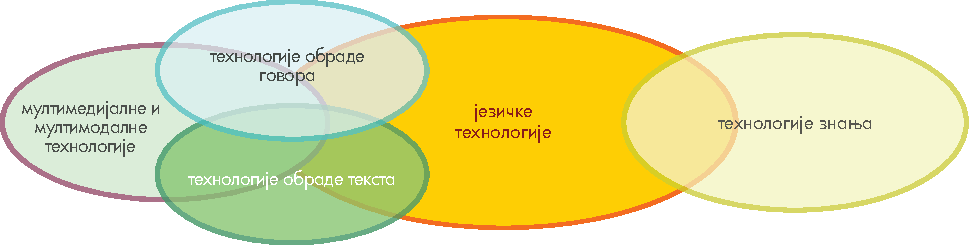
\includegraphics[width=\textwidth]{../_media/serbian/language_technologies}
  \caption{Контекст језичких технологија}
  \label{fig:ltincontext_sr}
  \colorrule{grey3}{\textwidth}{1.5pt}
\end{figure*}

У тексту који следи размотрићемо главне области примене језичких технологија, а то су  језичке провере, претраживање веба, технологију говора и машинско превођење. Ово укључује апликације и основне технологије као што су:
\begin{itemize}
 \item исправљање правописних грешака;
 \item подршка састављању текста;
 \item рачунарски потпомогнуто учење језика;
 \item претраживање информација;
\item  екстракција информација;
 \item одговори на питања;
\item резимирање текста;
\item препознавање говора, и
\item  синтеза говора.
\end{itemize}
Језичке технологије представљају добро дефинисану истраживачку област са обимном општом литературом. Заинтересовани читаоци се упућују на следеће референце:  \cite{jurafsky-martin01},  \cite{manning-schuetze1},  \cite{lt-survey1}.

Пре него што размотримо наведене  области примене,  укратко ћемо објаснити архитектуру типичног језичкотехнолошког система.

% --------------------------------------------------------------------------
 \subsection {Архитектуре апликација}
   
Типичне софтверске апликације за обраду језика састоје се од неколико компонената, које одражавају различите аспекте језика. Слика \ref{fig:textprocessingarch_sr} приказује веома поједностављену архитектуру на коју се може наићи у типичном систему за обраду текста. Прва три модула обрађују структуру и значење улазног текста:

\begin{figure*}[htb]
  \colorrule{grey3}{\textwidth}{1.5pt}
  \center
  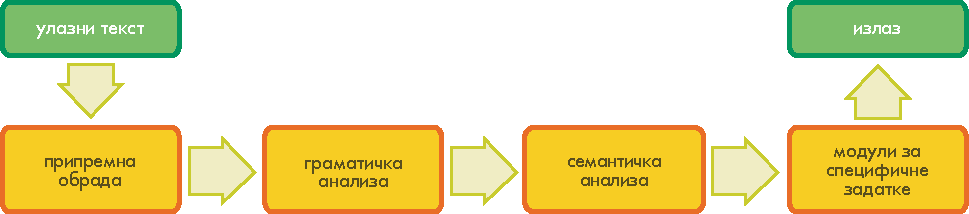
\includegraphics[width=\textwidth]{../_media/serbian/text_processing_app_architecture}
  \caption{Типична архитектура система за обраду текста}
  \label{fig:textprocessingarch_sr}
  \colorrule{grey3}{\textwidth}{1.5pt}
\end{figure*}

\begin{enumerate}
\item Претходна обрада: чишћење података, анализирање или уклањање форматирања и откривање улазног језика. У српском језику овај модул може да помогне у разрешавању ћириличко-латиничког двојства, као и екавско-ијекавског двојства. 
\item Граматичка анализа: проналажење глагола и његових објеката, модификатора и осталих конституената, као и откривање структуре реченице. 
\item Семантичка анализа: разрешавање вишезначности (тј. утврђивање одговарајућег значења речи у датом контексту); разрешавање анафора (тј. на шта се односе заменице) и референци у изразима; и представљање значења у машински читљивом облику.
\end{enumerate}

Након анализе текста, модули посвећени специфичним задацима о\-бав\-ља\-ју многе различите операције, као што су аутоматско резимирање и прегледање база података. Овај поједностављен и идеализован опис архитектуре апликација илуструје сложеност апликација језичких технологија. 

Пошто уведемо основна поља примене, даћемо кратак преглед стања у истраживању и образовању за језичке технологије, а закључићемо прегледом прошлих и текућих истраживачких програма. На крају овог одељка представићемо како по проценама стручњака изгледа позиција основних језичких алата и ресурса у простору чије димензије мере доступност, зрелост, квалитет и слично. 
Општа ситуација језичких технологија за српски језик резимирана је табелом \ref{tab:podrska}. 

% --------------------------------------------------------------------------
 \subsection {Основна поља примене}
   
   У овом одељку посветићемо пажњу најважнијим језичкотехнолошким алатима и ресурсима и даћемо преглед активности на подручју језичких технологија у Србији. % --------------------------------------------------------------------------
 \subsubsection {Провера језика}
   
Свако ко користи алат за обраду речи какав је Microsoft Word наишао је на компоненту за проверу, која указује на грешке у правопису и нуди исправке. Први програми за исправку правописних грешака поредили су листу речи извађених из текста са речником правилно исписаних речи. Данас су ти програми постали веома напредни. Коришћењем језички зависних алгоритама за \textbf{граматичка анализа} неки од њих могу да препознају грешке везане за морфологију (нпр. облици множине), синтаксу, као што је недостајање глагола, неслагање глагола са субјектом у лицу, броју и роду, на пример у ‘\textit{*Они је писало писмо.}’ Па ипак, већина програма за проверу правописа неће пронаћи грешке у следећем тексту \cite{ZAR}: 

\begin{quote}
 I have a spelling checker, \\
 It came with my PC. \\
 It plane lee marks four my revue \\
 Miss steaks aye can knot sea.  \\
\end{quote}
 
\vspace{-0.5cm}

Да би се могле уочити овакве грешке, у многим случајевима је потребна и анализа контекста. На пример: да ли реч треба да буде написана великим словом у српском језику или не: 

\begin{quote}
Дивио се \textit{Ружи}. [He admired \textit{Rose}.] \\
Дивио се \textit{ружи}. [He admired \textit{the rose}.] \\
\end{quote}

 
\vspace{-0.5cm}

Да би се ово постигло, могу се користити \textbf{граматике} специфичне за дати језик, што захтева много рада врхунских стручњака да би се оне уградиле у софтвер, или се могу користити такозвани статистички језички модели. Такви модели се заснивају на израчунавању вероватноће да се одређена реч појави у специфичном окружењу (нпр., испред или иза одређених речи). На пример, секвенција речи \textit{плава лагуна} много је вероватнија од секвенције \textit{плава Лагуна} (\textit{Лагуна} је издавач). Статистички језички модели се могу аутоматски извести из велике количине (исправних) језичких података (који се зову \textbf{текстуални корпуси}). До сада су ови приступи коришћени и процењивани за податке на енглеском језику. Они се, међутим, не могу увек директно применити на српски језик имајући у виду његов слободан ред речи и богату флексију.  

\vspace{-0.5cm}
\boxtext{Провера језика се не користи само у алатима за обраду текста; она се примењује и у системима за подршку писању.}

Први покушаји да се развије софтвер за проверу правописа за српски језик учињени су још крајем 1970-их \cite{UROSEVIC}  и били су мотивисани проблемима на које су наилазиле велике издавачке куће. Данас је слободан модул за проверу правописа за српски језик доступан за OpenOffice \cite{OpenOffice} на различитим оперативним системима, а постоји и занатски израђени производ, пакет RAS \cite{RASPROG}, који је развила компанија Srbosof и који се мора засебно инсталирати за сваког корисника. 

\begin{figure*}[htb]
  \colorrule{grey3}{\textwidth}{1.5pt}
  \center
  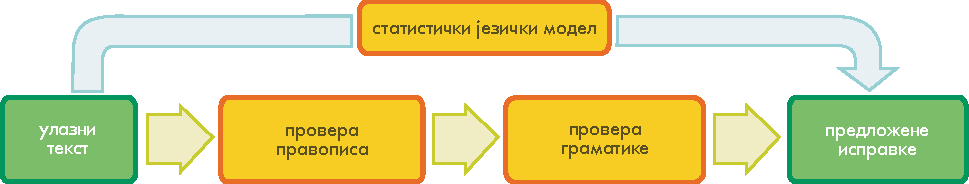
\includegraphics[width=\textwidth]{../_media/serbian/language_checking}
  \caption{Провера језика (статистичка; заснована на правилима)}
  \label{fig:langcheckingaarch_sr}
  \colorrule{grey3}{\textwidth}{1.5pt}
\end{figure*}

Провера језика се не користи само у алатима за обраду речи; она се примењује и у ,,системима за подршку писању текста'', тј. софтверским окружењима у којима се пишу приручници и друга документација за сложене производе информационих технологија, здравствене заштите, инжењерства и др. Плашећи се жалби купаца због погрешног коришћења и захтева за одштетом до којих би могло доћи јер су инструкције за употребу биле лоше или их они нису добро разумели, компаније су почеле све више пажње да посвећују техничкој документацији усредсређујући се истовремено на међународно тржиште (кроз превод или локализацију). Напредак у обради природних језика довео је до стварања софтвера за подршку писању текста који помаже ауторима техничке документације да користе речник и реченичне структуре усклађене са правилима струке и да поштују терминолошка ограничења која њихова компанија намеће. 

Провера језика није потребна само у системима за проверу правописа и за подршку писању текста већ је важна и за рачунарски потпомогнуто учење језика, а примењује се и  за аутоматску корекцију упита који се постављају машинама за претраживање веба, као што су Гуглови предлози типа 'Да ли сте мислили на...' 
 
% --------------------------------------------------------------------------
 \subsubsection {Претраживање веба}


\begin{figure*}[htb]
  \colorrule{grey3}{\textwidth}{1.5pt}
  \center
  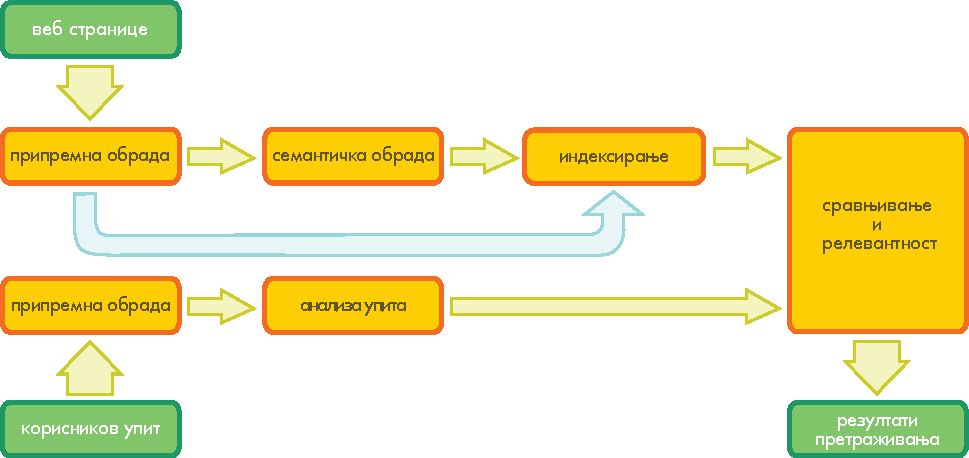
\includegraphics[width=\textwidth]{../_media/serbian/web_search_architecture}
  \caption{Претраживање веба}
  \label{fig:websearcharch_sr}
  \colorrule{grey3}{\textwidth}{1.5pt}
\end{figure*}

Данас је претраживање веба, интранета и дигиталних библиотека вероватно најраспрострањеније коришћење језичких технологија, које је ипак недовољно развијено. Машина за претраживање Гугл (Google), која је отпочела са радом 1998, данас се користи за око 80\% свих упита на вебу широм света \cite{SPIEGEL}. Глаголи ,,гуглати/изгуглати'' су у редовној употреби у српском језику. Ни сумеђа (интерфејс) за претраживање ни приказ пронађених резултата нису се значајно променили од прве верзије. У текућој верзији Гугл нуди могућност исправке погрешно написаних речи, а такође је уградио и основне могућности за семантичку претрагу које могу да побољшају тачност претраге анализирањем значења упитних термина у контексту \cite{PCWORLD}.  Успех Гугла показује да уз велику количину расположивих података и уз коришћење ефикасних техника за индексирање тих података, приступ који се заснива углавном на статистици може да доведе до задовољавајућих резултата.  

Па ипак, за озбиљније захтеве за информацијама неопходно је укључивање и дубљег лингвистичког знања за \textbf{семантичка анализа}. Експерименти са коришћењем \textbf{лексичких ресурса} као што су \textbf{тезауруси} у машински читљивом облику и \textbf{онтолошки језички ресурси} (нпр. WordNet за енглески или СрпНет за српски), доводили су до побољшања у проналажењу страница коришћењем синонимних термина, нпр. \textit{атомска енергија} и \textit{нуклеарна енергија}, или претраживањем преко још слабије повезаних термина какви су \textit{бели лук} и \textit{чешњак}. 

\boxtext{Следећа генерација претраживачких машина мораће да укључи много напреднију језичку технологију.} 

Следећа генерација машина за претраживање ће морати да укључи још много напредније језичке технологије, посебно да би могле да се изборе са упитима који се састоје од питања или неке друге врсте реченице уместо од листе кључних речи. На пример, за корисников упит \textit{Дај ми листу компанија које су преузете од стране других компанија у последњих пет година}, језичкотехнолошки систем мора да анализира реченицу на синтаксичком и семантичком нивоу, као и да обезбеди индекс који омогућава брзо проналажење релевантних докумената. За добијање задовољавајућег одговора треба да се примени синтаксичко парсирање да би се анализирала граматичка структура реченице и да би се утврдило да се траже компаније које су преузете, а не оне које су преузеле друге компаније. Такође, израз \textit{у последњих пет година} треба да се обради да би се утврдило на које се године односи. Коначно, упит који се обрађује треба да се сравни са огромном количином неструктурираних података да би се пронашли делићи информација које корисник тражи. Ово се обично назива ,,проналажење информација'', што укључује претраживање и рангирање релеватнијих докумената. Осим тога, да би се генерисала листа компанија, потребно је да се из документа  изваде информације да се одређена ниска речи односи на име компаније. Овај процес зове се ,,препознавање именованих ентитета''. 


Још захтевнији су покушаји сравњивања упита са документима који су записани на различитим језицима. За вишејезично проналажење информација потребно је да се аутоматски преведе упит на све могуће изворне језике, а затим да се пронађена информација преведе на циљни језик. 

Све већи проценат података је доступан у формату који није текстуалан, што повећава захтеве за сервисима који омогућавају мултимедијално проналажење информација, нпр. проналажење информација у сликама и аудио и видео подацима. За аудио и видео датотеке то укључује модул за препознавање говора, да би се конвертовао говорни садржај у текст или фонетску репрезентацију са којом се корисников упит може сравњивати. 

Популарне локације у Србији које нуде могућности претраживања, као што су B92 и Крстарица, ослањају се углавном на сервисе Гугла \cite{ALEXA}. Покушај да се уведе машина за претраживање која би обављала искључиво претрагу надоле домена .rs и која би била делимично прилагођена специфичним својствима српског језика напуштен је 2010. године као непрофитабилан. Одређен број малих и средњих предузећа ради на проширивању претраживачких сервиса, али углавном за стране партнере и за енглески језик. 

У истраживачком окружењу су обављени експерименти са системима за проширивање упита који су машинама за претраживање слали упите прошириване морфолошким речницима и вишејезичним семантичким мрежама. Ови експерименти су дали занимљиве и корисне резултате \cite{PAPINENI} у разноврсним доменима. 

% --------------------------------------------------------------------------
 \subsubsection {Говорна интеракција}
   
Говорна интеракција је једно од многих подручја примене која зависе од говорне технологије, тј. технологија за обраду говорног језика. Технологија говорне интеракције је основа за израду сумеђа  које дозвољавају кориснику да комуницира са машинама користећи говорни језик уместо графичког дисплеја, тастатуре или миша. Данас се такве гласовне корисничке сумеђе (voice user interfaces - VUIs) обично користе за потпуно или делимично аутоматизоване сервисе које компаније преко телефона нуде корисницима, запосленима или партнерима. Пословни домени који се у великој мери ослањају на гласовну корисничку сумеђу јесу банкарство, логистика, јавни превоз и телекомуникације. Технологија за говорну интеракцију се осим тога користи и за сумеђе са одређеним уређајима, нпр. у навигационим системима у колима, и за коришћење говора као алтернативе графичким или осетљивим на додир корисничким сумеђама, нпр. у паметним телефонима. 

\begin{figure*}[htb]
  \colorrule{grey3}{\textwidth}{1.5pt}
  \center 
  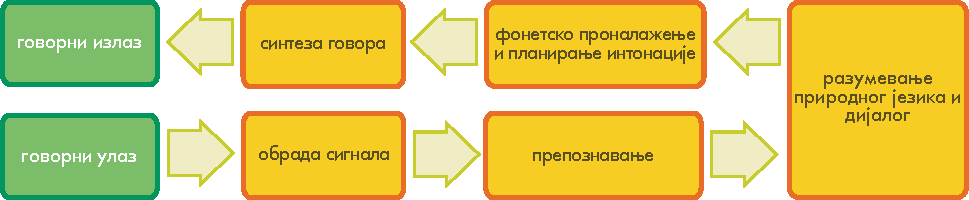
\includegraphics[width=\textwidth]{../_media/serbian/simple_speech-based_dialogue_architecture}
  \caption{Дијалошки систем заснован на говору}
  \label{fig:dialoguearch_sr}
  \colorrule{grey3}{\textwidth}{1.5pt}
\end{figure*}   


Говорна интеракција састоји се од четири технологије: 
\begin{enumerate}
\item Аутоматско \textbf{препознавање говора} (Automatic speech recognition  - ASR) је задужено за утврђивање које речи су стварно изговорене када је дата секвенција звукова коју је произвео корисник. 
\item Разумевање природног језика подразумева  анализу синтаксичке структуре корисниковог исказа и његову интерпретацију у складу са наменом одређеног система.
\item Управљање дијалогом одређује коју акцију треба предузети за дати корисников улаз и дате функционалности система. 
\item \textbf{Синтеза говора} (текст у говор, или Text-to-Speech, TTS) се користи за трансформацију одговора система у звукове које ће корисник примити као излаз. 
\end{enumerate}
Главни изазов је поседовање система за аутоматско препознавање говора који препознаје речи које је корисник изговорио што је прецизније могуће. Ово захтева или да се ограничи опсег могућих корисникових исказа на ограничен скуп кључних речи или да се ручно изграде језички модели који покривају широки опсег корисникових исказа на природном језику. Коришћењем техника машинског учења, језички модели могу да се изграђују аутоматски из \textbf{говорних корпуса}, тј. великих колекција говорних аудио датотека и њихових текстуалних транскрипција. Ограничавање исказа даје као резултат прилично ригидну и нефлексибилну  гласовну корисничку сумеђу коју корисници невољно прихватају. С друге стране, креирање, подешавање и одржавање богатих језичких модела може значајно да увећа трошкове. Па ипак, гласовне корисничке сумеђе  које користе језичке моделе који на почетку дозвољавају кориснику да слободно изразе своје намере -- подстакнути, на пример питањем \textit{Како Вам могу помоћи?} -- показују већи степен аутоматизованости и прихватања. 

\boxtext{Технологија говора је основа за изградњу сумеђа које омогућују кориснику да комуницира говорним језиком уместо преко графичког дисплеја, тастатуре или миша. }

За генерисање излазног дела гласовне корисничке сумеђе компаније теже коришћењу унапред снимљених исказа професионалних говорника. За статичке исказе код којих коришћене речи не зависе од конкретног контекста у коме се користе нити од личних података датог корисника, резултат може бити за корисника сасвим задовољавајући. Међутим, што је садржај исказа динамичнији, утолико више може да расте корисниково незадовољство због лоше прозодије до које долази  због спајања појединачних аудио-датотека. Насупрот томе, данашњи системи за трансформацију текста у говор су супериорнији у погледу прозодијске природности динамичких исказа, иако их је још потребно оптимизовати. 

Сумеђе на тржишту говорне интеракције су значајно стандардизоване у току последње деценије када су у питању њихове различите технолошке компоненте. Дошло је и до велике консолидације тржишта, посебно у домену система за аутоматско препознавање говора и за претварање текста у говор. На овом пољу, националним тржиштима земаља G20 -- што значи економски јаких земаља са значајном популацијом -- доминира свега 5 актера из целог света, при чему су Nuance  (САД) и Loquendo (Италија) најприсутнији у Европи. У 2011. год. Nuance  је објавио преузимање Loquendo, што представља даљи корак у консолидацији тржишта.

Методе за препознавање и синтезу говора су у Србији, као и на ширем простору бивше Југославије, развијане углавном у електроинжењерском окружењу уз сарадњу стручњака за фонетику. Први напори су били усмерени на препознавање изолованих фонема. Значајан помак је у овом домену учинила група са Техничког факултета Универзитета у Новом Саду када је израдила, поред говорних база података, лексичку базу од преко 4 милиона акцентованих облика речи српског језика и више од 3 милиона облика речи хрватског језика. Коришћењем ових ресурса развијене су различите апликације из домена аутоматског препознавања говора и претварања текста у говор. Препознавање и синтеза говора за српски су ушли у комерцијалну употребу кроз фирму AlfaNum, која је потекла са Универзитета у Новом Саду. Ова компанија успешно послује и у другим државама које су настале на простору бивше Југославије – у Хрватској, Македонији, Босни и Херцеговини и Црној Гори. Компанија AlfaNum има значајан број корисника међу српским компанијама. 

Када преводи на српски, Гуглов преводилац такође нуди основне могућности претварања текста у говор за резултате превођења, али без уграђених акцената. 

Гледајући даље од данашњег технолошког стања, може се рећи да ће доћи до значајних промена захваљујући ширењу паметних телефона као нове платформе за управљање корисничким односима, која ће се користити поред већ постојећих канала – телефона, интернета и електронске поште. Ова тенденција ће утицати и на коришћење технологије за говорну интеракцију. С једне стране, на дуже стазе ће опадати потражња за гласовном корисничком сумеђом за телефонске услуге. С друге стране, коришћење говорних могућности за приступачан улаз за паметне телефоне добиће на значају. Ову тенденцију подржава напредак који се већ може уочити у тачности препознавања говора независних говорника помоћу говорних сервиса за диктирање који се већ нуде као централизоване услуге корисницима паметних телефона. 

% --------------------------------------------------------------------------
 \subsubsection {Машинско превођење}
   

\begin{figure*}[htb]
  \colorrule{grey3}{\textwidth}{1.5pt}
  \center
  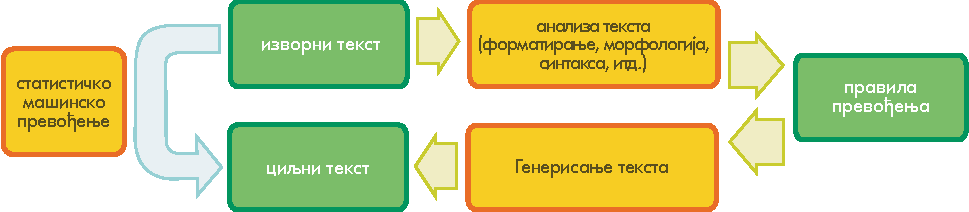
\includegraphics[width=\textwidth]{../_media/serbian/machine_translation}
  \caption{Машинско превођење (статистичко; засновано на правилима)}
  \label{fig:mtarch_sr}
  \colorrule{grey3}{\textwidth}{1.5pt}
\end{figure*}

Идеја да би се дигитални рачунари могли користити за превођење природних језика настала је 1946, после чега је уследило значајно финансирање истраживања у овој области педесетих година и потом осамдесетих година прошлог века. И поред свега, \textbf{машинско превођење} (Machine Translation - MT) и даље не успева да испуни велика очекивања која је подстакло у тим раним данима. 

\boxtext{На основном нивоу, машинско превођење једноставно замењује речи једног природног језика речима другог језика. }

На основном нивоу, машинско превођење једноставно замењује речи из једног природног језика речима из неког другог. Ово може да буде корисно у неким предметним доменима који користе веома ограничен формализован језик, као што је језик временских прогноза. Међутим, за добар превод текстова који нису толико стандардизовани, треба сравнити веће текстуалне јединице (фразе, реченице или целе пасусе) са најближим паром у циљном језику. Овде највећа потешкоћа лежи у томе што су природни језици вишезначни, што ствара изазове на различитим нивоима, јер треба, на пример, отклонити вишезначност речи на лексичком нивоу (,,јагуар'' може да буде назив животиње и аутомобила) или утврдити повезаност предлошких фраза на синтаксичком нивоу, као у:

\begin{itemize} 
\item \textit{Полицајац је успео да примети човека без двогледа}. \textit{[The policeman caught sight of the man without binoculars.]}
\item \textit{Полицајац је успео да примети човека без револвера.} \textit{[The policeman caught sight of  the man without the revolver.]}
\end{itemize}
Један начин да се изгради систем машинског превођења заснива се на лингвистичким правилима. За превођење између сродних језика могуће је и директно превођење у случајевима који наликују наведеним примерима. Ипак, системи засновани на правилима (или на знању) анализирају улазни текст и креирају посредну симболичку интерпретацију, из које се потом генерише текст на циљном језику. Успех ових метода веома зависи од постојања исцрпних лексикона са морфолошким, синтаксичким и семантичким информацијама, и великих скупова граматичких правила које су пажљиво израдили искусни лингвисти. Ово је веома дуг и скуп процес.

Како је крајем осамдесетих година прошлог века снага рачунара порасла и појефтинила, дошло је до већег интересовања за статистичке методе у машинском превођењу. Статистички модели се изводе из анализе двојезичних текстуалних корпуса, какав је, на пример, \textbf{паралелни корпус} Europarl, који садржи текстове Европског парламента на 21 језика. Под условом да постоји довољно података, статистичко машинско превођење може да изведе довољно добро приближно значење текста на страном језику, тако што обрађује паралелне верзије и проналази прихватљиве речи. Међутим, за разлику од система заснованих на знању, статистичко машинско превођење (или превођење засновано на подацима) често генерише неграматички излаз. С друге стране, осим што захтева мање људског напора за писање граматика, превођење засновано на подацима  може да покрије специфичности језика које измичу системима заснованим на знању, као што су идиоматски изрази. 

Пошто се јаке и слабе стране машинских система заснованих на знању, односно подацима, допуњују, истраживачи данас једногласно теже хибридним приступима који комбинују обе методологије. То се може урадити на више начина. Један начин је да се користе и системи засновани на знању и системи засновани на подацима, а да засебан модул за селекцију одлучи шта је најбољи излаз за сваку реченицу. Међутим, за дугачке реченице, дуже од, рецимо, дванаест речи, код оваквог приступа ни један резултат неће бити савршен. Боље је решење које комбинује најбоље делове сваке реченице добијене из различитих извора, што може бити доста сложено јер није увек очигледно шта су одговарајући делови код вишеструких могућности и јер их, осим тога, треба и поравнати. 

\boxtext{Машинско превођење представља посебан изазов за српски језик.}

Што се тиче везе српског и страних језика, проблеми зависе од природе специфичног језика (да ли има развијену морфологију, да ли има слободну или фиксирану дистрибуцију реченичних конституената, да ли користи чланове, да ли је записан ћириличним или латиничним писмом, да ли користи логичку или граматичку интерпункцију итд.). Међутим, овде се не ради само о томе шта су проблеми већ и о могућности да се сарађује на решавању сличних проблема. У том смислу би сарадња са пројектима везаним за рачунарску обраду других словенских језика била посебно корисна. Овде су такође важне лексичке и терминолошке везе, наиме у коликој мери је неки страни језик утицао на развој српског. У овом подручју би требало тражити сарадњу са пројектима чији је циљ рачунарска обрада оних језика који су служили и још увек служе као кичма развоја српског, а то су, пре свега, енглески, француски, немачки и руски.

Требало би додати да се одвијају и контрастивна истраживања српског и неких страних језика. Нажалост, има недовољно сарадње између лингвиста који се баве српским као матерњим језиком и оних лингвиста који се као стручњаци за стране језике укључују у контрастивна истраживања. Други проблем је недовољан број великих двојезичних речника. 

Највећа потреба за језичким технологијама у Србији је на пољу превођења. Постоје нека специјализована друштва (Друштво књижевних преводилаца Србије, Друштво научних и стручних преводилаца Србије), нека локална мала и средња предузећа (нпр. Elitence и Proverbum) и неке стране компаније (нпр. World\-Lingo) које нуде професионалне преводилачке услуге или слободан машински превод заснован на фразама (нпр. Google Translate, World\-Lingo). Неке од њих користе власничке електронске речнике за свој рад, а World\-Lingo нуди и шире услуге машинског превођења (веб локације, текст, документа, електронске поруке, API итд.).

Осим добро познатог и слободно доступног Гугловог статистичког система за превођење, који укључује и српски, ниједан други систем за машинско превођење за српски није произведен, осим неких почетних радова (нпр. у оквиру пројекта SEE-ERA) и малих експерименталних система.

Међутим, генерички статистички системи за машинско превођење какав је Google Translate подржавају српски у значајној мери, посебно за превођење на енглески и са енглеског. Ипак, за друге језичке парове перформансе су слабе, а добијени превод је често неразумљив, а понекад и смешан. То је резултат недовољне величине паралелних корпуса који је за те језичке парове коришћен за обуку система за статистичко машинско превођење. 

Још увек се сматра да се много може урадити на побољшању квалитета система за машинско превођење. Изазови обухватају прилагођавање језичких ресурса датом предметном или корисничком домену и укључивање терминолошких база и преводилачких меморија у постојеће радне процесе.  


\begin{figure*}[tb]
  \centering
  \setlength{\tabcolsep}{0.17em}
  \small
  \begin{tabular}{>{\columncolor{corange1}}cccccccccccccccccccccccc}
    & \multicolumn{22}{>{\columncolor{corange1}}c}{SERBIAN -- \textcolor{grey1}{Target language}}\\\addlinespace[{-.009cm}]
    \rowcolor{corange1}  & EN & BG & DE & CS & DA & EL & ES & ET & FI & FR & HU & IT & LT & LV & MT & NL & PL & PT & RO & SK & SL & SV\\
    EN & -- & \textcolor{blue}{40.5} & \textcolor{blue}{46.8} & \textcolor{green2}{52.6} & \textcolor{green2}{50.0} & \textcolor{blue}{41.0} & \textcolor{green2}{55.2} & \textcolor{purple}{34.8} & \textcolor{purple}{38.6} & \textcolor{green2}{50.1} & \textcolor{purple}{37.2} & \textcolor{green2}{50.4} & \textcolor{purple}{39.6} & \textcolor{blue}{43.4} & \textcolor{purple}{39.8} & \textcolor{green2}{52.3} & \textcolor{blue}{49.2} & \textcolor{green2}{55.0} & \textcolor{blue}{49.0} & \textcolor{blue}{44.7} & \textcolor{green2}{50.7} & \textcolor{green2}{52.0}\\
    BG & \textcolor{green}{61.3} & -- & \textcolor{purple}{38.7} & \textcolor{purple}{39.4} & \textcolor{purple}{39.6} & \textcolor{purple}{34.5} & \textcolor{blue}{46.9} & \textcolor{red3}{25.5} & \textcolor{red3}{26.7} & \textcolor{blue}{42.4} & \textcolor{red3}{22.0} & \textcolor{blue}{43.5} & \textcolor{red3}{29.3} & \textcolor{red3}{29.1} & \textcolor{red3}{25.9} & \textcolor{blue}{44.9} & \textcolor{purple}{35.1} & \textcolor{blue}{45.9} & \textcolor{purple}{36.8} & \textcolor{purple}{34.1} & \textcolor{purple}{34.1} & \textcolor{purple}{39.9}\\
    DE & \textcolor{green2}{53.6} & \textcolor{red3}{26.3} & -- & \textcolor{purple}{35.4} & \textcolor{blue}{43.1} & \textcolor{purple}{32.8} & \textcolor{blue}{47.1} & \textcolor{red3}{26.7} & \textcolor{red3}{29.5} & \textcolor{purple}{39.4} & \textcolor{red3}{27.6} & \textcolor{blue}{42.7} & \textcolor{red3}{27.6} & \textcolor{purple}{30.3} & \textcolor{red2}{19.8} & \textcolor{green2}{50.2} & \textcolor{purple}{30.2} & \textcolor{blue}{44.1} & \textcolor{purple}{30.7} & \textcolor{red3}{29.4} & \textcolor{purple}{31.4} & \textcolor{blue}{41.2}\\
    CS & \textcolor{green2}{58.4} & \textcolor{purple}{32.0} & \textcolor{blue}{42.6} & -- & \textcolor{blue}{43.6} & \textcolor{purple}{34.6} & \textcolor{blue}{48.9} & \textcolor{purple}{30.7} & \textcolor{purple}{30.5} & \textcolor{blue}{41.6} & \textcolor{red3}{27.4} & \textcolor{blue}{44.3} & \textcolor{purple}{34.5} & \textcolor{purple}{35.8} & \textcolor{red3}{26.3} & \textcolor{blue}{46.5} & \textcolor{purple}{39.2} & \textcolor{blue}{45.7} & \textcolor{purple}{36.5} & \textcolor{blue}{43.6} & \textcolor{blue}{41.3} & \textcolor{blue}{42.9}\\
    DA & \textcolor{green2}{57.6} & \textcolor{red3}{28.7} & \textcolor{blue}{44.1} & \textcolor{purple}{35.7} & -- & \textcolor{purple}{34.3} & \textcolor{blue}{47.5} & \textcolor{red3}{27.8} & \textcolor{purple}{31.6} & \textcolor{blue}{41.3} & \textcolor{red3}{24.2} & \textcolor{blue}{43.8} & \textcolor{red3}{29.7} & \textcolor{purple}{32.9} & \textcolor{red3}{21.1} & \textcolor{blue}{48.5} & \textcolor{purple}{34.3} & \textcolor{blue}{45.4} & \textcolor{purple}{33.9} & \textcolor{purple}{33.0} & \textcolor{purple}{36.2} & \textcolor{blue}{47.2}\\
    EL & \textcolor{green2}{59.5} & \textcolor{purple}{32.4} & \textcolor{blue}{43.1} & \textcolor{purple}{37.7} & \textcolor{blue}{44.5} & -- & \textcolor{green2}{54.0} & \textcolor{red3}{26.5} & \textcolor{red3}{29.0} & \textcolor{blue}{48.3} & \textcolor{red3}{23.7} & \textcolor{blue}{49.6} & \textcolor{red3}{29.0} & \textcolor{purple}{32.6} & \textcolor{red3}{23.8} & \textcolor{blue}{48.9} & \textcolor{purple}{34.2} & \textcolor{green2}{52.5} & \textcolor{purple}{37.2} & \textcolor{purple}{33.1} & \textcolor{purple}{36.3} & \textcolor{blue}{43.3}\\
    ES & \textcolor{green}{60.0} & \textcolor{purple}{31.1} & \textcolor{blue}{42.7} & \textcolor{purple}{37.5} & \textcolor{blue}{44.4} & \textcolor{purple}{39.4} & -- & \textcolor{red3}{25.4} & \textcolor{red3}{28.5} & \textcolor{green2}{51.3} & \textcolor{red3}{24.0} & \textcolor{green2}{51.7} & \textcolor{red3}{26.8} & \textcolor{purple}{30.5} & \textcolor{red3}{24.6} & \textcolor{blue}{48.8} & \textcolor{purple}{33.9} & \textcolor{green2}{57.3} & \textcolor{purple}{38.1} & \textcolor{purple}{31.7} & \textcolor{purple}{33.9} & \textcolor{blue}{43.7}\\
    ET & \textcolor{green2}{52.0} & \textcolor{red3}{24.6} & \textcolor{purple}{37.3} & \textcolor{purple}{35.2} & \textcolor{purple}{37.8} & \textcolor{red3}{28.2} & \textcolor{blue}{40.4} & -- & \textcolor{purple}{37.7} & \textcolor{purple}{33.4} & \textcolor{purple}{30.9} & \textcolor{purple}{37.0} & \textcolor{purple}{35.0} & \textcolor{purple}{36.9} & \textcolor{red3}{20.5} & \textcolor{blue}{41.3} & \textcolor{purple}{32.0} & \textcolor{purple}{37.8} & \textcolor{red3}{28.0} & \textcolor{purple}{30.6} & \textcolor{purple}{32.9} & \textcolor{purple}{37.3}\\
    FI & \textcolor{blue}{49.3} & \textcolor{red3}{23.2} & \textcolor{purple}{36.0} & \textcolor{purple}{32.0} & \textcolor{purple}{37.9} & \textcolor{red3}{27.2} & \textcolor{purple}{39.7} & \textcolor{purple}{34.9} & -- & \textcolor{red3}{29.5} & \textcolor{red3}{27.2} & \textcolor{purple}{36.6} & \textcolor{purple}{30.5} & \textcolor{purple}{32.5} & \textcolor{red2}{19.4} & \textcolor{blue}{40.6} & \textcolor{red3}{28.8} & \textcolor{purple}{37.5} & \textcolor{red3}{26.5} & \textcolor{red3}{27.3} & \textcolor{red3}{28.2} & \textcolor{purple}{37.6}\\
    FR & \textcolor{green}{64.0} & \textcolor{purple}{34.5} & \textcolor{blue}{45.1} & \textcolor{purple}{39.5} & \textcolor{blue}{47.4} & \textcolor{blue}{42.8} & \textcolor{green}{60.9} & \textcolor{red3}{26.7} & \textcolor{purple}{30.0} & -- & \textcolor{red3}{25.5} & \textcolor{green2}{56.1} & \textcolor{red3}{28.3} & \textcolor{purple}{31.9} & \textcolor{red3}{25.3} & \textcolor{green2}{51.6} & \textcolor{purple}{35.7} & \textcolor{green}{61.0} & \textcolor{blue}{43.8} & \textcolor{purple}{33.1} & \textcolor{purple}{35.6} & \textcolor{blue}{45.8}\\
    HU & \textcolor{blue}{48.0} & \textcolor{red3}{24.7} & \textcolor{purple}{34.3} & \textcolor{purple}{30.0} & \textcolor{purple}{33.0} & \textcolor{red3}{25.5} & \textcolor{purple}{34.1} & \textcolor{red3}{29.6} & \textcolor{red3}{29.4} & \textcolor{purple}{30.7} & -- & \textcolor{purple}{33.5} & \textcolor{red3}{29.6} & \textcolor{purple}{31.9} & \textcolor{red2}{18.1} & \textcolor{purple}{36.1} & \textcolor{red3}{29.8} & \textcolor{purple}{34.2} & \textcolor{red3}{25.7} & \textcolor{red3}{25.6} & \textcolor{red3}{28.2} & \textcolor{purple}{30.5}\\
    IT & \textcolor{green}{61.0} & \textcolor{purple}{32.1} & \textcolor{blue}{44.3} & \textcolor{purple}{38.9} & \textcolor{blue}{45.8} & \textcolor{blue}{40.6} & \textcolor{red3}{26.9} & \textcolor{red3}{25.0} & \textcolor{red3}{29.7} & \textcolor{green2}{52.7} & \textcolor{red3}{24.2} & -- & \textcolor{red3}{29.4} & \textcolor{purple}{32.6} & \textcolor{red3}{24.6} & \textcolor{green2}{50.5} & \textcolor{purple}{35.2} & \textcolor{green2}{56.5} & \textcolor{purple}{39.3} & \textcolor{purple}{32.5} & \textcolor{purple}{34.7} & \textcolor{blue}{44.3}\\
    LT & \textcolor{green2}{51.8} & \textcolor{red3}{27.6} & \textcolor{purple}{33.9} & \textcolor{purple}{37.0} & \textcolor{purple}{36.8} & \textcolor{red3}{26.5} & \textcolor{red3}{21.1} & \textcolor{purple}{34.2} & \textcolor{purple}{32.0} & \textcolor{purple}{34.4} & \textcolor{red3}{28.5} & \textcolor{purple}{36.8} & -- & \textcolor{blue}{40.1} & \textcolor{red3}{22.2} & \textcolor{purple}{38.1} & \textcolor{purple}{31.6} & \textcolor{purple}{31.6} & \textcolor{red3}{29.3} & \textcolor{purple}{31.8} & \textcolor{purple}{35.3} & \textcolor{purple}{35.3}\\
    LV & \textcolor{green2}{54.0} & \textcolor{red3}{29.1} & \textcolor{purple}{35.0} & \textcolor{purple}{37.8} & \textcolor{purple}{38.5} & \textcolor{red3}{29.7} & \textcolor{red2}{8.0} & \textcolor{purple}{34.2} & \textcolor{purple}{32.4} & \textcolor{purple}{35.6} & \textcolor{red3}{29.3} & \textcolor{purple}{38.9} & \textcolor{purple}{38.4} & -- & \textcolor{red3}{23.3} & \textcolor{blue}{41.5} & \textcolor{purple}{34.4} & \textcolor{purple}{39.6} & \textcolor{purple}{31.0} & \textcolor{purple}{33.3} & \textcolor{purple}{37.1} & \textcolor{purple}{38.0}\\
    MT & \textcolor{green}{72.1} & \textcolor{purple}{32.2} & \textcolor{purple}{37.2} & \textcolor{purple}{37.9} & \textcolor{purple}{38.9} & \textcolor{purple}{33.7} & \textcolor{blue}{48.7} & \textcolor{red3}{26.9} & \textcolor{red3}{25.8} & \textcolor{blue}{42.4} & \textcolor{red3}{22.4} & \textcolor{blue}{43.7} & \textcolor{purple}{30.2} & \textcolor{purple}{33.2} & -- & \textcolor{blue}{44.0} & \textcolor{purple}{37.1} & \textcolor{blue}{45.9} & \textcolor{purple}{38.9} & \textcolor{purple}{35.8} & \textcolor{blue}{40.0} & \textcolor{blue}{41.6}\\
    NL & \textcolor{green2}{56.9} & \textcolor{red3}{29.3} & \textcolor{blue}{46.9} & \textcolor{purple}{37.0} & \textcolor{blue}{45.4} & \textcolor{purple}{35.3} & \textcolor{blue}{49.7} & \textcolor{red3}{27.5} & \textcolor{red3}{29.8} & \textcolor{blue}{43.4} & \textcolor{red3}{25.3} & \textcolor{blue}{44.5} & \textcolor{red3}{28.6} & \textcolor{purple}{31.7} & \textcolor{red3}{22.0} & -- & \textcolor{purple}{32.0} & \textcolor{blue}{47.7} & \textcolor{purple}{33.0} & \textcolor{purple}{30.1} & \textcolor{purple}{34.6} & \textcolor{blue}{43.6}\\
    PL & \textcolor{green}{60.8} & \textcolor{purple}{31.5} & \textcolor{blue}{40.2} & \textcolor{blue}{44.2} & \textcolor{blue}{42.1} & \textcolor{purple}{34.2} & \textcolor{blue}{46.2} & \textcolor{red3}{29.2} & \textcolor{red3}{29.0} & \textcolor{blue}{40.0} & \textcolor{red3}{24.5} & \textcolor{blue}{43.2} & \textcolor{purple}{33.2} & \textcolor{purple}{35.6} & \textcolor{red3}{27.9} & \textcolor{blue}{44.8} & -- & \textcolor{blue}{44.1} & \textcolor{purple}{38.2} & \textcolor{purple}{38.2} & \textcolor{purple}{39.8} & \textcolor{blue}{42.1}\\
    PT & \textcolor{green}{60.7} & \textcolor{purple}{31.4} & \textcolor{blue}{42.9} & \textcolor{purple}{38.4} & \textcolor{blue}{42.8} & \textcolor{blue}{40.2} & \textcolor{green}{60.7} & \textcolor{red3}{26.4} & \textcolor{red3}{29.2} & \textcolor{green2}{53.2} & \textcolor{red3}{23.8} & \textcolor{green2}{52.8} & \textcolor{red3}{28.0} & \textcolor{purple}{31.5} & \textcolor{red3}{24.8} & \textcolor{blue}{49.3} & \textcolor{purple}{34.5} & -- & \textcolor{purple}{39.4} & \textcolor{purple}{32.1} & \textcolor{purple}{34.4} & \textcolor{blue}{43.9}\\
    RO & \textcolor{green}{60.8} & \textcolor{purple}{33.1} & \textcolor{purple}{38.5} & \textcolor{purple}{37.8} & \textcolor{blue}{40.3} & \textcolor{purple}{35.6} & \textcolor{green2}{50.4} & \textcolor{red3}{24.6} & \textcolor{red3}{26.2} & \textcolor{blue}{46.5} & \textcolor{red3}{25.0} & \textcolor{blue}{44.8} & \textcolor{red3}{28.4} & \textcolor{red3}{29.9} & \textcolor{red3}{28.7} & \textcolor{blue}{43.0} & \textcolor{purple}{35.8} & \textcolor{blue}{48.5} & -- & \textcolor{purple}{31.5} & \textcolor{purple}{35.1} & \textcolor{purple}{39.4}\\
    SK & \textcolor{green}{60.8} & \textcolor{purple}{32.6} & \textcolor{purple}{39.4} & \textcolor{blue}{48.1} & \textcolor{blue}{41.0} & \textcolor{purple}{33.3} & \textcolor{blue}{46.2} & \textcolor{red3}{29.8} & \textcolor{red3}{28.4} & \textcolor{purple}{39.4} & \textcolor{red3}{27.4} & \textcolor{blue}{41.8} & \textcolor{purple}{33.8} & \textcolor{purple}{36.7} & \textcolor{red3}{28.5} & \textcolor{blue}{44.4} & \textcolor{purple}{39.0} & \textcolor{blue}{43.3} & \textcolor{purple}{35.3} & -- & \textcolor{blue}{42.6} & \textcolor{blue}{41.8}\\
    SL & \textcolor{green}{61.0} & \textcolor{purple}{33.1} & \textcolor{purple}{37.9} & \textcolor{blue}{43.5} & \textcolor{blue}{42.6} & \textcolor{purple}{34.0} & \textcolor{blue}{47.0} & \textcolor{purple}{31.1} & \textcolor{red3}{28.8} & \textcolor{purple}{38.2} & \textcolor{red3}{25.7} & \textcolor{blue}{42.3} & \textcolor{purple}{34.6} & \textcolor{purple}{37.3} & \textcolor{purple}{30.0} & \textcolor{blue}{45.9} & \textcolor{purple}{38.2} & \textcolor{blue}{44.1} & \textcolor{purple}{35.8} & \textcolor{purple}{38.9} & -- & \textcolor{blue}{42.7}\\
    SV & \textcolor{green2}{58.5} & \textcolor{red3}{26.9} & \textcolor{blue}{41.0} & \textcolor{purple}{35.6} & \textcolor{blue}{46.6} & \textcolor{purple}{33.3} & \textcolor{blue}{46.6} & \textcolor{red3}{27.4} & \textcolor{purple}{30.9} & \textcolor{purple}{38.9} & \textcolor{red3}{22.7} & \textcolor{blue}{42.0} & \textcolor{red3}{28.2} & \textcolor{purple}{31.0} & \textcolor{red3}{23.7} & \textcolor{blue}{45.6} & \textcolor{purple}{32.2} & \textcolor{blue}{44.2} & \textcolor{purple}{32.7} & \textcolor{purple}{31.3} & \textcolor{purple}{33.5} & --\\
    \end{tabular}
  \caption{SERBIAN -- \textcolor{grey1}{Machine translation between 22 EU-languages \cite{euro1}}}
  \label{fig:euromatrix}
\end{figure*}


Акције за процењивање омогућавају да се пореде квалитет система за машинско превођење, различити приступи, као и статус система за машинско превођење за различите језичке парове. Следећа табела, представљена у оквиру пројекта Европске комисије Euromatrix+, приказује перформансе по паровима за 22 од 23 службена европска језика (недостаје ирски). Резултати су рангирани према BLEU процени, која даје више оцене за боље преводе \cite{PAPINENI}. Човек-преводилац постиже резултат од око 80 поена. 

Најбољи резултати (приказани зеленом и плавом бојом) постигнути су за језике који имају користи од значајних истраживачких напора у оквиру сарадничких програма и за које постоје многи паралелни корпуси (нпр., енглески, француски, холандски, шпански и немачки), а најлошији (приказани црвеном бојом) за језике који нису могли да користе сличне претходне напоре или који су веома различити од других језика (нпр., мађарски, малтешки, фински). 

% --------------------------------------------------------------------------
 \subsection {Друге области примене}
   
Изградња апликација заснованих на језичким технологијама укључује опсег подзадатака који се не виде увек на нивоу интеракције са корисником, али који обезбеђују значајне функционалности система ,,испод хаубе''. Сваки од њих представља важан истраживачки задатак који се развио у засебну поддисциплину у оквиру рачунарске лингвистике.

На пример, одговарање на питања је постало активно истраживачко подручје, за које су изграђени анотирани корпуси и отпочела су научна такмичења. Идеја је да се крене даље од претраживања заснованог на кључним речима (на које машине одговарају целом колекцијом релевантних одговора) ка ситуацији у којој корисник поставља конкретно питање, а систем пружа један одговор. На пример: 
\begin{itemize}
\item[] \textit{Питање: Са колико година је Нил Армстронг крочио на Месец?} 
\item[] \textit{Одговор: 38}. 
\end{itemize}

Иако је ово очигледно повезано са већ поменутим основним претраживањем веба, одговарање на питања је данас пре свега заједнички термин за различите истраживачке теме као што су: које типове питања треба разликовати и како треба с њима поступати, како треба анализирати и поредити документа која потенцијално садрже одговоре (да ли она садрже супротстављене одговоре?), и како се специфична информација – заправо одговор -  може поуздано извући из документа, не запостављајући при томе контекст у коме се налази. 

\boxtext{Примене језичке технологије често пружају значајне функционалности ,,иза сцене'' већих софтверских система. }

Ова област је повезана са задатком екстракције информација, облашћу која је била изузетно популарна и утицајна у време ,,статистичког заокрета'' у рачунарској лингвистици почетком деведесетих година. Циљ екстракције информација је да се идентификују специфични делићи информација у специфичним класама докумената; то може да буде, на пример, откривање кључних актера у преузимању компанија на основу извештавања у новинама. Други сценарио на коме се радило били су извештаји о терористичким инцидентима, где је проблем био да се текст преслика у шаблон у коме су спецификовани извршилац, мета, време и место инцидента, и шта је њиме постигнуто. Централна карактеристика екстракције информација је попуњавање шаблона специфичног за неки домен, због чега је то још један пример технологије ‘иза сцене’, која представља јасно разграничено истраживачко подручје, али која из практичних разлога мора да се угради у одговарајуће окружење апликације.  

Два ,,гранична'' подручја, која понекад имају улогу самосталне апликације, а понекад помоћне компоненте (,,испод хаубе''), јесу резимирање текста и \textbf{генерисање текста}. Резимирање се, очигледно, односи на задатак скраћивања дугачког текста, и њега као функцију нуди MS Word. Оно ради углавном на статистичким основама, тако што прво идентификује ,,важне'' речи у тексту (на пример, речи које се у конкретном тексту често јављају, док се у текстовима у начелу јављају много ређе), а затим утврђује у којим се реченицама јавља пуно важних речи. Ове реченице се затим издвајају из текста и из њих се саставља сажетак. У овом сценарију, који је комерцијално уобичајен, резимирање се своди на просту екстракцију реченица, а текст на подскуп својих реченица. Алтернативни приступ, коме се такође посвећују неки истраживачки напори, састоји се у генерисању потпуно нових реченица које не постоје у изворном тексту. Ово захтева дубље разумевање текста, што значи да је тај приступ (за сада) знатно мање робустан. Све у свему, генерисање текста у већини случајева није самостална апликација, већ је уграђено у шире софтверско окружење, као што је клинички информациони систем у коме се подаци о пацијентима скупљају, складиште и обрађују. Генерисање извештаја је само једна од многих примена резимирања текста. 

Унутар ових поменутих подручја се, кад је реч о српском, спроводе врло успешни експерименти везани за препознавање именованих ентитета, као дела проблема екстракције информација. Очекује се убрзани развој система за екстракцију информација и одговарање на питања, имајући у виду опсег изграђених морфолошких речника и локалних граматика. 

Постоје и друга подручја на којима се примењују језичке технологије. Једно од њих је откривање плагијаторства, које користи језички независне технологије, али се може проширити  претрагом за једноставним парафразама текста. Истраживање које иде у овом правцу за научне чланке у Србије је реализовала компанија CEON \cite{CEON}.

% --------------------------------------------------------------------------
 \subsection {Образовни програми}
 
Језичке технологије су интердисциплинарно подручје које захтева знања многих стручњака, лингвиста, стручњака за рачунарство, математичара, филозофа, психолингвиста и неуролога, да поменемо само неке. Као такво, оно још није добило сталну позицију у високом образовању у Србији и углавном је ограничено на појединачне курсеве у оквиру општијих постдипломских студијских програма. Парадоксално, упркос оваквом стању, у оквиру истраживачке станице Петница \cite{PETNICA} се сваке године организују мали истраживачки семинари за средњошколце са темама из рачунарске лингвистике. 

На нивоу универзитетских студија, теме из области рачунарске лингвистике су присутне на студијама из рачунарства, електронике, библиотекарства, лингвистике и психологије, и то на универзитетима у Београду и Новом Саду. Предмети који су понуђени студентима дају основне појмове о процесу обраде природних језика, али су у функцији формирања студената за друкчије профиле. На Математичком факултету у Београду, на редовним студијама су присутни курсеви из лексичке анализе и истраживање података (енгл. data mining), поред курсева који обрађују фундаментална математичка знања потребна у обради природних језика (посебно статистика, алгебра и логика), док на докторским студијама постоји већи избор предмета из области технологија природних језика. Најтемељније образовање на овом подручју стичу студенти Групе за библиотекарство и информатику на Филолошком факултету у Београду, док на другим групама тог факултета постоји највише један уводни курс. У оквиру студија српског језика није предвиђено образовање на подручју обраде природних језика. На Филозофским факултетима у Београду и Новом Саду, на групама за психологију постоје курсеви из психолингвистике на којима се студенти упознају са статистичким методама обраде језика. На техничким факултетима се изучавају методе од значаја за обраду говора. Курикулум који даје специјалност у домену рачунарске лингвистике или језичких технологија не постоји ни на једном од факултета. 

% --------------------------------------------------------------------------
 \subsection {Национални пројекти и иницијативе}
   
Индустрија језичких технологија је у Србији релативно неразвијена у поређењу са водећим економијама земаља Европске уније, и то из више разлога. Главна покретачка снага иза развоја језичких технологија у Србији су углавном домаћа мала и средња предузећа, али и неке стране компаније, које понекада обезбеђују подршку за српски језик у разноврсним апликацијама које траже подршку језичких технологија. Пошто не постоји национални програм подршке развоју језичких технологија, њихов развој и примена се одвијају често на некоординиран начин. Постоје бар три правца којима се језичке технологије уводе у Србију: (а) кроз државне научне и развојне пројекте, (б) преко (првенствено) страних фирми које уз рачунарску опрему пружају и одређени облик језичке подршке и (в) кроз интерни развој у оквиру домаћих организација какве су, нпр., издавачке куће или преводилачке агенције. Активности у ова три правца се одвијају, осим изузетно, независно једне од других. 

С друге стране, рачунарски писмено становништво у Србији је навикло да користи графичку корисничку сумеђу (интерфејс) на енглеском језику, иако неки од њих можда и не знају енглески. Локализоване верзије њима понекад изгледају чудне и непрецизне и нису вољни да их користе. Једине апликације које у великом броју користе  графичку корисничку сумеђу, на српском су различите пословне, финансијске и рачуноводствене апликације, укључујући и SAP ERP систем. Ипак, има примера локализоване графичке корисничке сумеђе познатих софтверских продаваца као што је Microsoft (нпр. MS Windows, MS Office), Google или Oracle (локализација Open Office, финансирана у периоду од 2008. до 2011. од стране Министарства за телекомуникације и информационо друштво кроз пројекат на Математичком факултету \cite{OO_MATF}).

\vspace{-1ex}
Научни пројекти које финансира Министарство за образовање и науку тек у најновијем циклусу научних пројеката (период 2011--2014) препознају интердисциплинарност. До 2010. године научни пројекти (па тиме и критеријуми за њихову евалуацију) били су оштро раздвојени на подручја математике (коме је подређено рачунарство), језика и технолошких дисциплина. У таквом амбијенту је било тешко реализовати природни спој дисциплина које су у основи развоја језичких технологија. У оваквом контексту било је неопходно успоставити везе између истраживања на подручју српског језика и информатике. 

Први такав пројекат, под називом „Интеракције текста и речника“, формиран је 2002. године као заједнички пројекат катедара за српски језик Филолошког факултета у Београду и Филозофског факултета у Новом Саду и Математичког факултета у Београду. У оквиру овог пројекта је формиран први корпус савременог српског језика \cite{KORPUS} доступан преко веба, а који данас има преко 300 корисника са различитих универзитета и института у земљи и иностранству. У оквиру овог пројекта је започета и конструкција електронског морфолошког речника српског језика према тзв. LADL формату \cite{KRSTEV}. Овај пројекат је настављен као заједнички пројекат Катедре за српски језик Филолошког факултета у Београду и Математичког факултета у периоду од 2006. до 2010. под називом ,,Теоријско-методолошки оквир за модернизацију описа српског језика'' и од 2011. до 2014. као ,,Српски језик и његови ресурси: теорија, опис и примене''. Кроз ове пројекте је довршена конструкција електронског речника простих речи и започет рад на конструкцији речника сложених речи, развијени су паралелни француско-српски и енглеско-српски корпус литерарних текстова, описане су локалне граматике за поједине сегменте српског (посебно за именоване ентитете), као и различити софтверски алати, од којих посебан значај има радна станица LeXimir, која омогућава интеграцију и трансформацију хетерогених лексичких ресурса. 

Упоредо са овим истраживањима у области језика, у области друштвених наука је финансиран пројекат ,,Фундаментални когнитивни процеси и функције'', који је реализован на Катедри за психологију Филозофског факултета у Београду. Овај пројекат је, поред осталог, имао за циљ да испита могућност аутоматске анотације текста полазећи од анотираног корпуса \cite{SRB_KORPUS}, развијеног још током педесетих година, а деведесетих преведеног у електронски облик. 

Синтеза и препознавање говора на Техничком факултету Универзитета у Новом Саду се реализује кроз пројекте технолошког развоја почев од 2005. године, и то ,,Развој говорних технологија на српском језику и њихова примена у ‘Телекому Србија’'' (2005--2007), ,,Говорна комуникација човек-машина'' (2008--2010),  ,,Развој дијалошких система за српски и друге јужнословенске језике'' (2011--2014).  Они пружају подршку различитим апликацијама и сервисима за претварање текста у говор и аутоматско препознавање говора, који укључују системе за интерактивне гласовне одговоре (IVR), пословне телефонске системе, позивне центре, пријављивање гласом, праћење реклама, уочавање речи, и др.

У оквиру других области науке развијани су појединачни ресурси од значаја за језичке технологије, али без непосредне интеракције са већ наведеним пројектима. Поменимо као примере геолошки српско-енглески тезаурус \cite{RGF} и фолклористичку базу ДАБИ Балканолошког института САНУ  \cite{BALKANINSTITUT}.

Упоредо са националним пројектима, српске научне институције су биле укључене и у различите међународне пројекте везане за подручје језичких технологија. Током периода санкција Уједињених нација, одржавање одређеног нивоа активности је било могуће захваљујући учешћу у пројектима TELRI I и II \cite{TELRI}. Иако српске истраживачке групе у то време нису могле да учествују на пројекту MULTEXT-East \cite{NL}, оне су ипак произвеле корисне ресурсе у формату који је тај пројекат дефинисао: морфосинтаксички опис српског језика, поравнату верзију српског превода романа ,,\textit{1984}'' Џорџа Орвела, његову лематизирану и морфосинтаксички етикетирану верзију и исцрпан речник који покрива комплетну лексику романа ,,\textit{1984}''. 

\boxtext{Ситуација у разним доменима обраде српског језика је различита, али значајан напредак постоји у развоју корпуса, морфолошкој анализи, електронским речницима, као и у екстракцији именованих ентитета (датуми, топоними итд.)}

По укидању санкција, посебно је значајан био пројекат BalkaNet \cite{CORDIS}, који је омогућио развој семантичке мреже типа WordNet за српски. Кроз билатералну сарадњу са Француском је развијен српски део вишејезичне лексичке базе властитих имена Prolex \cite{CNRTL}, а у оквиру пројекта Intera једномилионски паралелизовани енглеско-српски корпус, који је лематизиран и морфолошки анотиран. Овај корпус је послужио за обучавање тагера и за експерименте у поравнавању на нивоу речи и у аутоматском превођењу.

Српски учесници су били укључени у два регионална пројекта. Један од њих, SEE-ERA.NET - Building Language Resources and Translation Models for Machine Translation (Изградња језичких ресурса и преводилачких модела за машинско превођење), био је усмерен на јужнословенске и балканске језике (ICT 10503 RP, 2007--2008). Његов главни допринос био је развој једносмерних преводилачких модела који се ослањају на вишејезичке ресурсе великих димензија, у ствари на корпус \textit{Acquis Communautaire}.  Међутим, пошто документа која улазе у овај ресурс у то време још нису била преведена на српски, преводилачки модел није био произведен за српски. Превод законске регулативе Европске уније је у току и део преведеног материјала је већ доступан \cite{PREVODJENJE}. Са своје стране је српски тим допринео овом пројекту развојем једног другог вишејезичног ресурса који се заснива на роману Жила Верна ,,\textit{Пут око света за осамдесет дана}'' (у том тренутку било је укључено 16 језика). Други пројекат био је WISE - An Electronic Marketplace to Support Pairs of Less Widely Studied European Languages (Електронско тржиште за подршку паровима мање изучаваних европских језика), чији је циљ била производња не само вишејезичних лексичких ресурса обогаћених лингвистичким метаподацима већ и изградња и промоција електронског тржишта за слабије изучаване балканске језике, укључујући и српски (BSEC 009 / 05.2007, 2007 -- 2008).

Даље активности подразумевају, пре свега, развој поступака за синтаксичку анализу српског, која је, с обзиром на слободан ред речи и морфолошко богатство српског језика, изузетно сложен поступак. Ово подразумева развој нових ресурса, пре свега нових типова речника и корпуса, као и пратећих алата.
 
% --------------------------------------------------------------------------
 \subsection {Доступност алата и ресурса}
   
Табела \ref{tab:podrska} даје приказ текућег стања језичких технологија за српски језик. Рангирање постојећих алата и ресурса се заснива на процени више водећих експерата који су дали оцене на скали 0 (врло ниско) до 6 (врло високо) на основу седам критеријума. 



% Begin table
\begin{table*}[ht]
\centering

\begin{tabular}{>{\columncolor{orange1}}p{.33\linewidth}@{\hspace*{6mm}}c@{\hspace*{6mm}}c@{\hspace*{6mm}}c@{\hspace*{6mm}}c@{\hspace*{6mm}}c@{\hspace*{6mm}}c@{\hspace*{6mm}}c}
\rowcolor{orange1}
 \cellcolor{white}&
 \begin{sideways}\makecell[l]{Квантитет}\end{sideways} &
 \begin{sideways}\makecell[l]{\makecell[l]{Доступност} }\end{sideways} &
 \begin{sideways}\makecell[l]{Квалитет}\end{sideways} &
 \begin{sideways}\makecell[l]{Покривеност}\end{sideways} &
 \begin{sideways}\makecell[l]{Зрелост}\end{sideways} &
 \begin{sideways}\makecell[l]{Одрживост}\end{sideways} &
 \begin{sideways}\makecell[l]{Прилагодљивост}\end{sideways} \\ \addlinespace

\multicolumn{8}{>{\columncolor{orange2}}l}{\textcolor{black}{Језичке технологије (алати, технологије, апликације)}} \\ \addlinespace

Препознавање говора	&2&2&1&1&1&1&0 \\ \addlinespace
Синтеза говора &2&2&4&4&5&5&1\\ \addlinespace 
Граматичка анализа&1&1&2,5&2&2&1,5&1,5\\ \addlinespace
Семантичка анализа &1&1&1&1,5&1&1&1,5\\ \addlinespace
Генерисање текста &0&0&0&0&0&0&0\\ \addlinespace
Машинско превођење &1&1&0&1&0&1&1\\ \addlinespace

\multicolumn{8}{>{\columncolor{orange2}}l}{\textcolor{black}{Језички ресурси (ресурси, подаци, базе знања)}} \\ \addlinespace

Текстуални корпуси &0,5&1&0,5&1&1&1&0,5\\ \addlinespace
Говорни корпуси &1&2&4&4&3&3&3\\ \addlinespace
Паралелни корпуси &3&3&3&2&2&2&3\\ \addlinespace
Лексички ресурси &1&2&2&2&2&2&2,5\\ \addlinespace
Граматике &1&1&0&1&0&1&1\\
\end{tabular}
\caption{Стање језичких технологија за српски језик}
\label{tab:podrska}
\end{table*}

За српски језик, стање ресурса и технологија може се описати на следећи начин:
\begin{itemize}
\item Што се тиче морфолошких и с њима повезаних питања, може се слободно рећи да је ниво развоја технологија и ресурса задовољавајући, углавном захваљујући постојању великог електронског речника и локалних граматика. Непосредна последица тога је да су потребни алати за проналажење информација и екс\-трак\-ци\-ју информација на располагању. Неки од речника су спремни за широку употребу, док неке још треба доградити, на пример СрпНет.
\item Референтни корпус савременог српског језика екавског изговора је на располагању, као и неколико поравнатих корпуса, и сви они су на располагању истраживачима српског језика. Текућа истраживања су усредсређена на доградњу референтног корпуса и његово проширивање ијекавским изговором. 
\item Говорне технологије су добро развијене и нашле су широке пословне примене, али се истраживања морају ширити да би се проширила и поља примене.
\item Софтвер намењен повећавању продуктивности лексикографа је развијен, али недовољна спремност за нове технологије у традиционално оријентисаном лексикографском окружењу је препрека бржем развоју лексикографије. 
\item У неким подручјима су обављени успешни експерименти у строго истраживачком окружењу, као што је плитко парсирање, резимирање, машинско превођење, онтолошки ресурси. Међутим, добијени резултати су још увек далеко од нивоа развоја који је постигнут за развијене европске језике. Пажњу истраживача привлаче и мултимедијални и мултимодални документи, посебно у контексту дигитализације културног наслеђа.
\end{itemize}
Имајући у виду сложеност српске синтаксе, подручја заснована на дубоком парсирању једноставно не постоје: семантика реченица, семантика текста, генерисање језика. Због тога не постоји ни формализована синтакса српског, што ограничава развој синтактички и семантички анотираних корпуса. Формализација синтаксе српског је према томе најхитнији задатак за даљи развој језичких технологија.


% --------------------------------------------------------------------------
 \subsection {Поређење језика}
   
Текуће стање подршке језичких технологија значајно се разликује од једне језичке заједнице до друге. Да би се упоредиле ситуације у којима се налазе различити језици, овај одељак ће представити оцену засновану на два примера области примене (машинско превођење и обрада говора) и на једној технологији (анализа текста), као и на основним ресурсима неопходним за изградњу апликација језичких технологија.
Језици су сврстани у групе на основу следеће скале од пет вредности:
\begin{itemize}
\item Одлична подршка језичким технологијама
\item Добра подршка
\item Умерена подршка
\item Фрагментарна подршка
\item Слаба подршка или без подршке 
\end{itemize}
Мера подршке језичким технологијама установљена је на основу следећих критеријума:
\begin{itemize}
\item \textbf{Обрада говора}: Квалитет постојећих технологија за препознавање говора, квалитет постојећих технологија за синтезу говора, покривеност домена, број и обим постојећих говорних корпуса, бројност и разноврсност расположивих апликација заснованих на говору
\item \textbf{Машинско превођење}: Квалитет постојећеих технологија машинског превођења, број покривених језичких парова, покривеност језичких феномена и домена, квалитет и обим постојећих паралелних корпуса, бројност и разноврсност расположивих апликација машинског превођења 
\item \textbf{Анализа текста}: Квалитет постојећих технологија за анализу текста и области које покривају (морфологија, синтакса, семантика), покривеност језичких феномена и домена, бројност и разноврсност расположивих апликација, квалитет и обим постојећих (анотираних) текстуалних корпуса, квалитет постојећих лексичких ресурса и граматика и области које покривају (нпр. WordNet)
\item \textbf{Ресурси}: Квалитет и обим постојећих текстуалних, говорних и паралелних корпуса, квалитет постојећих лексичких ресурса и граматика и области које покривају
\end{itemize} 


Горње табеле показују да су алати и ресурси за српски језик углавном у најнижој групи. Српски добро стоји у поређењу са језицима са малим бројем говорника, као што су хрватски, словеначки и словачки, али сви ти језици су далеко иза заступљенијих европских језика као што су немачки или француски. Па ипак, чак ни за ове последње језике, алати и ресурси  језичких технологија нису достигли квалитет и покривеност одговарајућих алата и ресурса за енглески језик, који је у врху у свим областима језичке технологије. А и у енглеским језичким ресурсима постоји још увек доста празнина с тачке гледишта апликација високог квалитета.



% --------------------------------------------------------------------------
 \subsection {Закључци}
   
\textit{У овој серији белих књига учинили смо значајан почетни напор да оценимо подршку језичких технологија за 30 европских језика и да обезбедимо квалитетно поређење тих језика. Пошто су идентификоване потребе и недостаци, заједница европских језичких технологија, као и све заинтересоване стране сада су у прилици да осмисле програме истраживања и развоја широких размера чији је циљ изградња истински вишејезичне,  технолошки оспособљене Европе}.

Видели смо да постоје огромне разлике између европских језика. Док за неке језике у одређеним областима примене постоје квалитетни ресурси и  одговарајући софтвер, за друге језике ту постоје значајне празнине. Многим језицима недостају основе технологије за анализу текста, као и суштински ресурси за развој тих технологија. Други имају основне ресурсе или алате, али још увек нису у прилици да инвестирају у семантичку обраду. Зато нам тек предстоји да учинимо главни напор за постизање амбициозног циља обезбеђивања високо квалитетног машинског превођења између свих европских језика.  

Обим ресурса и опсег алата који постоје за српски језик још увек су врло ограничени, нарочито када се упореде са алатима и ресурсима за језике као што су француски, немачки и посебно енглески, и нису довољни ни по квалитету ни по квантитету за развој оне врсте технологије која је неопходна за подршку истински вишејезичном друштву знања. 

Технологије које су већ развијене и оптимизоване за енглески не могу једноставно да се пренесу на српски језик. Систем за синтаксичку анализу структуре реченице заснован на енглеском по правилу је неприкладан за примену на српском тексту. Рад на обради српског језика до сада је био концентрисан на развој ресурса и алата који су у складу са специфичним својствима српског (пре свега опис његове богате морфологије). Овај правац развоја мора обавезно да се задржи и у будућности. 

За скромну језичку заједницу и истраживачку средину као што је српска, сарадња у развоју ресурса, како на домаћем тако и на међународном нивоу,  од пресудног је значаја. Ово генерално  важи за већину словенских језика, а за сарадњу су неопходне даље стимулативне мере. Посебно велике могућности за сарадњу постоје између пројеката везаних за стандардне језике штокавског порекла, као и за словенске језике уопште, имајући у виду заједничка својства тих језика. 

Учешће Србије у CESAR-у и META-NET-у требало би да допринесе развоју, стандардизацији и доступности неколико важних ресурса језичких технологија и стога развоју језичких технологија за српски језик. Дугорочни циљ META-NET-а јесте да уведе технологију високог квалитета за све језике како би се постигло политичко и економско јединство кроз културну разноврсност. Технологија ће помоћи да се уклоне постојеће баријере и да се изграде мостови међу европским језицима. Ово захтева од свих заинтересованих страна – у политици, истраживању, привреди и друштву – да уједине своје напоре за будућност. 

Индустрија српских језичких технологија је веома скромна. Укључено је тек неколико средњих и малих предузећа и њихов приступ је у суштини заснован на примени ,,грубе силе'', што значи да се у основи занемарују специфичности српског језика. Наши налази показују да је једина алтернатива улагање значајних напора у стварање ресурса за језичке технологије за српски и њихово коришћење за унапређење истраживања, иновација и развоја. С обзиром на потребу за великим количинама података и екстремну сложеност система језичких технологија, од виталног је значаја развој нове инфраструктуре и кохерентније организације истраживања, која би подстакла већу сарадњу. Други кључни допринос био би успостављање мул\-ти\-дис\-ци\-пли\-нар\-ног студијског програма обраде језика на мастер и докторском нивоу, што данас не постоји.

Према томе, можемо да закључимо да постоји неодложна потреба за широком, координираном иницијативом усмереном на превазилажење разлика у спремности језичких технологија за европске језике као целину. 


\begin{table*}[ht]
\small
\centering
\begin{tabular}
{ % defines color for each column.
>{\columncolor{corange5}} p{.17\linewidth}@{\hspace{.027\linewidth}}
>{\columncolor{corange4}}p{.17\linewidth}@{\hspace{.027\linewidth}}
>{\columncolor{corange3}}p{.17\linewidth}@{\hspace{.027\linewidth}}
>{\columncolor{corange2}}p{.17\linewidth}@{\hspace{.027\linewidth}}
>{\columncolor{corange1}}p{.17\linewidth} 
}
\rowcolor{orange1} % redefines color for all columns in row 1 
  \multicolumn{1}{>{\columncolor{white}}c@{\hspace{.040\linewidth}}}{\textbf{одлична}} & 
  \multicolumn{1}{@{}>{\columncolor{white}}c@{\hspace{.040\linewidth}}}{\textbf{добра}} &
  \multicolumn{1}{@{}>{\columncolor{white}}c@{\hspace{.040\linewidth}}}{\textbf{умерена}} &
  \multicolumn{1}{@{}>{\columncolor{white}}c@{\hspace{.040\linewidth}}}{\textbf{фрагментарна}} &
  \multicolumn{1}{@{}>{\columncolor{white}}c}{\textbf{слаба или без}} \\ 
  \multicolumn{1}{>{\columncolor{white}}c@{\hspace{.040\linewidth}}}{\textbf{подршка}} & 
  \multicolumn{1}{@{}>{\columncolor{white}}c@{\hspace{.040\linewidth}}}{\textbf{подршка}} &
  \multicolumn{1}{@{}>{\columncolor{white}}c@{\hspace{.040\linewidth}}}{\textbf{подршка}} &
  \multicolumn{1}{@{}>{\columncolor{white}}c@{\hspace{.040\linewidth}}}{\textbf{подршка}} &
  \multicolumn{1}{@{}>{\columncolor{white}}c}{\textbf{подршка}} \\ \addlinespace

& \vspace*{0.5mm}енглески
& \vspace*{0.5mm}немачки \newline   
италијански \newline  
фински \newline 
француски \newline 
холандски \newline 
португалски \newline 
шпански \newline
чешки \newline 
& \vspace*{0.5mm}баскијски \newline 
бугарски \newline 
дански \newline 
естонски \newline 
галицијски\newline 
грчки \newline  
ирски \newline  
каталонски \newline 
норвешки \newline 
пољски \newline 
шведски \newline
\textbf{српски} \newline 
словачки \newline 
словеначки \newline 
мађарски  \newline
& \vspace*{0.5mm}исландски \newline  
хрватски \newline 
летонски \newline 
литвански \newline 
малтешки \newline 
румунски\\
\end{tabular}
\label{fig:obrada_govora}
\caption{Језичке групе за обраду говора}
\end{table*}

\begin{table*}[ht]
\small
\centering
\begin{tabular}
{ % defines color for each column.
>{\columncolor{corange5}} p{.17\linewidth}@{\hspace{.027\linewidth}}
>{\columncolor{corange4}}p{.17\linewidth}@{\hspace{.027\linewidth}}
>{\columncolor{corange3}}p{.17\linewidth}@{\hspace{.027\linewidth}}
>{\columncolor{corange2}}p{.17\linewidth}@{\hspace{.027\linewidth}}
>{\columncolor{corange1}}p{.17\linewidth} 
}
\rowcolor{orange1} % redefines color for all columns in row 1
 \multicolumn{1}{>{\columncolor{white}}c@{\hspace{.040\linewidth}}}{\textbf{одлична}} & 
  \multicolumn{1}{@{}>{\columncolor{white}}c@{\hspace{.040\linewidth}}}{\textbf{добра}} &
  \multicolumn{1}{@{}>{\columncolor{white}}c@{\hspace{.040\linewidth}}}{\textbf{умерена}} &
  \multicolumn{1}{@{}>{\columncolor{white}}c@{\hspace{.040\linewidth}}}{\textbf{фрагментарна}} &
  \multicolumn{1}{@{}>{\columncolor{white}}c}{\textbf{слаба или без}} \\ 
  \multicolumn{1}{>{\columncolor{white}}c@{\hspace{.040\linewidth}}}{\textbf{подршка}} & 
  \multicolumn{1}{@{}>{\columncolor{white}}c@{\hspace{.040\linewidth}}}{\textbf{подршка}} &
  \multicolumn{1}{@{}>{\columncolor{white}}c@{\hspace{.040\linewidth}}}{\textbf{подршка}} &
  \multicolumn{1}{@{}>{\columncolor{white}}c@{\hspace{.040\linewidth}}}{\textbf{подршка}} &
  \multicolumn{1}{@{}>{\columncolor{white}}c}{\textbf{подршка}} \\ \addlinespace

& \vspace*{0.5mm} енглески 
& \vspace*{0.5mm} француски \newline 
шпански
& \vspace*{0.5mm}немачки \newline 
италијански \newline 
каталонски \newline 
холандски \newline 
пољски \newline 
румунски \newline 
мађарски 
& \vspace*{0.5mm}баскијски \newline 
бугарски \newline 
дански \newline 
естонски \newline 
фински \newline 
галицијски \newline 
грчки \newline 
ирски \newline 
исландски \newline 
хрватски \newline 
летонски \newline 
литвански \newline 
малтешки \newline 
норвешки \newline 
португалски \newline 
шведски \newline 
\textbf{српски} \newline 
словачки \newline 
словеначки \newline 
чешки \newline
\end{tabular}
\label{fig:masinsko_prevodjenje}
\caption{Језичке групе за машинско превођење}
\end{table*}

\begin{table*}[ht]
  \small
  \centering
  \begin{tabular}
{ % defines color for each column.
>{\columncolor{corange5}} p{.17\linewidth}@{\hspace{.027\linewidth}}
>{\columncolor{corange3}}p{.17\linewidth}@{\hspace{.027\linewidth}}
>{\columncolor{corange3}}p{.17\linewidth}@{\hspace{.027\linewidth}}
>{\columncolor{corange2}}p{.17\linewidth}@{\hspace{.027\linewidth}}
>{\columncolor{corange1}}p{.17\linewidth} 
}
\rowcolor{orange1} % redefines color for all columns in row 1
 \multicolumn{1}{>{\columncolor{white}}c@{\hspace{.040\linewidth}}}{\textbf{одлична}} & 
  \multicolumn{1}{@{}>{\columncolor{white}}c@{\hspace{.040\linewidth}}}{\textbf{добра}} &
  \multicolumn{1}{@{}>{\columncolor{white}}c@{\hspace{.040\linewidth}}}{\textbf{умерена}} &
  \multicolumn{1}{@{}>{\columncolor{white}}c@{\hspace{.040\linewidth}}}{\textbf{фрагментарна}} &
  \multicolumn{1}{@{}>{\columncolor{white}}c}{\textbf{слаба или без}} \\ 
  \multicolumn{1}{>{\columncolor{white}}c@{\hspace{.040\linewidth}}}{\textbf{подршка}} & 
  \multicolumn{1}{@{}>{\columncolor{white}}c@{\hspace{.040\linewidth}}}{\textbf{подршка}} &
  \multicolumn{1}{@{}>{\columncolor{white}}c@{\hspace{.040\linewidth}}}{\textbf{подршка}} &
  \multicolumn{1}{@{}>{\columncolor{white}}c@{\hspace{.040\linewidth}}}{\textbf{подршка}} &
  \multicolumn{1}{@{}>{\columncolor{white}}c}{\textbf{подршка}} \\ \addlinespace

& \vspace*{0.5mm}енглески
& \vspace*{0.5mm}немачки \newline 
  француски \newline 
  италијански \newline 
  холандски \newline 
 шпански
& \vspace*{0.5mm}баскијски \newline 
  бугарски \newline 
  дански \newline 
  фински \newline 
  галицијски \newline 
  грчки \newline 
  каталонски \newline 
  норвешки \newline 
  пољски \newline 
  португалски \newline 
  румунски \newline 
 шведски \newline 
  словачки \newline 
  словеначки \newline 
  чешки \newline 
  мађарски \newline 
& \vspace*{0.5mm}естонски \newline 
  ирски \newline 
  исландски \newline 
  хрватски \newline 
  летонски \newline 
  литвански \newline 
  малтешки \newline 
  \textbf{српски} \\
  \end{tabular}
\label{fig:analiza_teksta}
\caption{Језичке групе за анализу текста}
\end{table*}

\begin{table*}[ht]
  \small
  \centering
\begin{tabular}
{ % defines color for each column.
>{\columncolor{corange5}} p{.17\linewidth}@{\hspace{.027\linewidth}}
>{\columncolor{corange4}}p{.17\linewidth}@{\hspace{.027\linewidth}}
>{\columncolor{corange3}}p{.17\linewidth}@{\hspace{.027\linewidth}}
>{\columncolor{corange2}}p{.17\linewidth}@{\hspace{.027\linewidth}}
>{\columncolor{corange1}}p{.17\linewidth} 
}
\rowcolor{orange1} % redefines color for all columns in row 1

 \multicolumn{1}{>{\columncolor{white}}c@{\hspace{.040\linewidth}}}{\textbf{одлична}} & 
  \multicolumn{1}{@{}>{\columncolor{white}}c@{\hspace{.040\linewidth}}}{\textbf{добра}} &
  \multicolumn{1}{@{}>{\columncolor{white}}c@{\hspace{.040\linewidth}}}{\textbf{умерена}} &
  \multicolumn{1}{@{}>{\columncolor{white}}c@{\hspace{.040\linewidth}}}{\textbf{фрагментарна}} &
  \multicolumn{1}{@{}>{\columncolor{white}}c}{\textbf{слаба или без}} \\ 
  \multicolumn{1}{>{\columncolor{white}}c@{\hspace{.040\linewidth}}}{\textbf{подршка}} & 
  \multicolumn{1}{@{}>{\columncolor{white}}c@{\hspace{.040\linewidth}}}{\textbf{подршка}} &
  \multicolumn{1}{@{}>{\columncolor{white}}c@{\hspace{.040\linewidth}}}{\textbf{подршка}} &
  \multicolumn{1}{@{}>{\columncolor{white}}c@{\hspace{.040\linewidth}}}{\textbf{подршка}} &
  \multicolumn{1}{@{}>{\columncolor{white}}c}{\textbf{подршка}} \\ \addlinespace
    
& \vspace*{0.5mm}енглески
& \vspace*{0.5mm}немачки \newline 
    француски \newline 
    холандски \newline 
 шведски \newline 
    чешки \newline 
    мађарски  \newline
   пољски \newline 
  италијански \newline 
   шпански 
& \vspace*{0.5mm} баскијски\newline 
    бугарски\newline 
    дански \newline 
    естонски \newline 
    фински \newline 
    галицијски \newline 
    грчки \newline 
    каталонски \newline 
    хрватски \newline 
    норвешки \newline 
    португалски \newline 
    румунски \newline 
    \textbf{српски} \newline 
    словачки \newline 
    словеначки \newline
&  \vspace*{0.5mm} ирски \newline 
    исландски \newline 
    летонски \newline 
    литвански \newline 
    малтешки  \\
  \end{tabular}
  \label{fig:resursi}
  \caption{Језичке групе за ресурсе}
\end{table*}

 
\end{multicols}

\clearpage

% --------------------------------------------------------------------------
 \ssection[МЕТА-НЕТ (META-NET)] {МЕТА-НЕТ (META-NET)}
 \begin{multicols}{2}

\parindent20pt

МЕТА-НЕТ је мрежа изврсности коју финансира Европска унија. Њу тренутно чини 54 члана, који представљају 33 европске земље. МЕТА-НЕТ подстиче технолошки савез вишејезичне Европе (Multilingual Europe Technology Alliance - META), нарастајућу заједницу професионалаца и организација са подручја језичких технологија из Европе. 

МЕТА-НЕТ сарађује са другим великим иницијативама, каква је CLARIN, која потпомаже успостављање информатизације хуманистичких истраживања. МЕТА-НЕТ је посвећен остваривању технолошких основа за успостављање и одржавање правог вишејезичног европског информационог друштва које:
\begin{itemize}
\item омогућава комуникацију и сарадњу на више језика, 
\item обезбеђује једнак приступ информацијама и знању на свим језицима,
\item нуди напредне и приступачне могућности умрежене информационе технологије свим европским грађанима.
\end{itemize}
МЕТА-НЕТ стимулише и промовише вишејезичне технологије за све европске језике. Технологије омогућавају аутоматско превођење, генерисање садржаја, обраду информација, у\-прав\-ља\-ње знањем за широк распон апликација и предметних области. Мрежа жели да побољша текуће приступе, да би дошло до боље комуникације и сарадње међу језицима. Европљани имају једнако право на информације и знање без обзира којим језиком се служе. 

\vspace{-3ex}
% --------------------------------------------------------------------------
 \subsection {Правци активности}
   

МЕТА-НЕТ је покренут 1. фебруара 2010. са циљем да се унапреди истраживање језичких технологија. Мрежа подржава Европу која се удружује у јединствено дигитално тржиште и информациони простор. МЕТА-НЕТ је покренуо више активности које доприносе остварењу његових циљева. МЕТА-ВИЗИЈА, МЕТА-РАЗМЕНА и МЕТА-ИСТРАЖИВАЊЕ су три правца активности ове мреже. 

\vspace{3ex}
\textbf{МЕТА-ВИЗИЈА (META-VISION)} подстиче заједницу динамичних и утицајних заинтересованих страна да се удруже око заједничке визије и заједничког стратешког истраживачког плана (Strategic Research Agenda - SRA). Главни задатак ове активности је да изгради кохерентну и повезану заједницу за језичке технологије у Европи повезујући представнике крајње расцепканих и разноврсних група заинтересованих страна. У првој години постојања МЕТА-НЕТА презентације на скуповима су биле концентрисане на предочавање јавности циљева МЕТА-НЕТА: на FLaReNet форуму у Шпанији, Данима језичких технологија у Луксембургу, JIAMCATT-у 2010. у Луксембургу, LREC-у 2010. на Малти, EAMT-у 2010. у Француској и ICT-у 2010. у Белгији.  Према првим проценама, МЕТА-НЕТ је већ ступио у контакт са више од 2500 стручњака за језичке технологије да би са њима поделио своје циљеве и визије. На МЕТА-ФОРУМУ 2010. у Бриселу, МЕТА-НЕТ је поделио почетне резултате изградње својих визија са више од 250 учесника. У серији интерактивних сесија добијен је одзив учесника на визије које је мрежа представила. 
   
\textbf{МЕТА-РАЗМЕНА (META-SHARE)} ствара отворене, широко распрострањене погодности за заједничко коришћење и размену ресурса. Мрежа репозиторијума \textit{једнак с једнаким} (peer-to-peer) садржаће језичке податке, алате и веб услуге документоване метаподацима високог квалитета и организоване у стандардизоване категорије. Ресурсима се може у сваком тренутку приступити, а претражују се на униформан начин. Расположиви ресурси укључују материјале отвореног кода слободне за коришћење, као и ограничене, комерцијално доступне компоненте на бази плаћања. МЕТА-РАЗМЕНА је усмерена на постојеће језичке податке, алате и системе, као и на нове производе и оне у настајању, неопходне за изградњу и евалуацију нових технологија, производа и услуга. Поновна употреба, комбиновање, поновно постављање циља и поновно конструисање језичких података и алата игра кључну улогу. МЕТА-РАЗМЕНА ће на крају постати незаобилазни део тржишта језичких технологија за развојне тимове, експерте за локализацију, истраживаче, преводиоце и језичке стручњаке из малих, средњих и великих предузећа. МЕТА-РАЗМЕНА покрива цео развојни циклус језичких технологија – од истраживања до иновативних производа и услуга. Кључни аспект ове активности је успостављање МЕТА-РАЗМЕНЕ као значајног и драгоценог дела европске и глобалне инфраструктуре за језичкотехнолошку заједницу.
   
 
   
\textbf{МЕТА-ИСТРАЖИВАЊЕ (META-RESEARCH)} успоставља мостове ка релевантним сродним технолошким областима. Ова активност настоји да искористи напредак у другим областима и да употреби иновативна истраживања која могу да допринесу језичким технологијама. Посебно, ова активност жели да унесе више семантике у машинско превођење, оптимизује поделу рада у хибридном машинском превођењу, користи контекст при аутоматском превођењу и припрема искуствену основу за машинско превођење. МЕТА-ИСТРАЖИВАЊЕ сарађује са другим областима и дисциплинама, као што су машинско учење и семантички веб. МЕТА-ИСТРАЖИВАЊЕ се фокусира на прикупљање података, припрему скупова података и организовање језичких ресурса за потребе евалуације, на састављање инвентара алата и метода и на  организовање радионица и обуке за чланове заједнице. Ова активност је већ јасно идентификовала аспекте машинског превођења у којима семантика може да утиче на текућу најбољу праксу. Поред тога, активност је створила препоруке о томе како да се приступи проблему интегрисања семантичких информација у машинско превођење. МЕТА-ИСТРАЖИВАЊЕ приводи крају нови језички ресурс за машинско превођење, анотирани хибридни обучени корпус за машинско превођење који обезбеђује податке за енглеско-немачки, енглеско-шпански и енглеско-чешки језички пар. МЕТА-ИСТРАЖИВАЊЕ је развило и софтвер за прикупљање вишејезичких корпуса скривених на вебу.

\end{multicols}

\cleardoublepage

\addtocontents{toc}{\protect\clearpage\protect}
\addtocontents{toc}{\protect\thispagestyle{empty}\protect}
\addtocontents{toc}{\protect\vspace*{4mm}\protect}
\addtocontents{toc}{\smallskip{\Large\textsf{\centerline{SERBIAN LANGUAGE IN DIGITAL AGE}}\par}}

\setcounter{section}{0}
\setcounter{figure}{0}
\setcounter{table}{0}

\cleardoublepage

\selectlanguage{english}

\ssection[Executive Summary]{Executive Summary}

\begin{multicols}{2}

    
During the last 60 years, Europe has become a distinct political and economic structure, yet culturally and linguistically it is still very diverse. This means that from Portuguese to Polish and Italian to Icelandic, everyday communication between Europe’s citizens as well as communication in the spheres of business and politics is inevitably confronted by language barriers. The EU’s institutions spend about a billion euros a year on maintaining their policy of multilingualism, i.\,e.~translating texts and interpreting spoken communication. Yet does this have to be such a burden? Modern language technology and linguistic research can make a significant contribution to pulling down these linguistic borders. When combined with intelligent devices and applications, language technology will in the future be able to help Europeans talk easily to each other and do business with each other even if they do not speak a common language. 

\boxtext{Language technology\penalty-10000\ builds bridges for Europe’s future.}

Major trade partners of Serbia come from the EU, with a share of over 50\% in its total trade, while exports to the EU market are free-of-customs according to the Stabilisation and Association Agreement. But language barriers can bring business to a halt, especially for SMEs who do not have the financial means to reverse the situation. The only (unthinkable) alternative to this kind of multilingual Europe would be to allow a single language to take a dominant position and end up replacing all other languages. 

One classic way of overcoming the language barrier is to learn foreign languages. Yet without technological support, mastering the 23 official languages of the member states of the European Union and some 60 other European languages is an insurmountable obstacle for the citizens of Europe and its economy, political debate, and scientific progress.   

The solution is to build key enabling technologies. These will offer European actors tremendous advantages, not only within the common European market but also in trade relations with third countries, especially emerging economies.  To achieve this goal and preserve Europe’s cultural and linguistic diversity, it is necessary to first carry out a systematic analysis of the linguistic particularities of all European languages, and the current state of language technology support for them. Language technology solutions will eventually serve as a unique bridge between Europe’s languages. 

\boxtext{Language technology as a key for the future}

The automated translation and speech processing tools currently available on the market still fall short of this ambitious goal. The dominant actors in the field are primarily privately-owned for-profit enterprises based in Northern America. Already in the late 1970s, the EU realised the profound relevance of language technology as a driver of European unity, and began funding its first research projects, such as EUROTRA. At the same time, national projects were set up that generated valuable results but never led to concerted European action. In contrast to this highly selective funding effort, other multilingual societies such as India (22 official languages) and South Africa (11 official languages) have recently set up long-term national programmes for language research and technology development.
 
The predominant actors in LT today rely on imprecise statistical approaches that do not make use of deeper linguistic methods and knowledge. For example, sentences are automatically translated by comparing a new sentence against thousands of sentences previously translated by humans. The quality of the output largely depends on the amount and quality of the available sample corpus. While the automatic translation of simple sentences in languages with sufficient amounts of available text material can achieve useful results, such shallow statistical methods are doomed to fail in the case of languages with a much smaller body of sample material or in the case of sentences with complex structures.

The European Union has therefore decided to fund projects such as EuroMatrix and EuroMatrixPlus (since 2006) and iTranslate4 (since 2010), which carry out basic and applied research and generate resources for establishing high quality language technology solutions for all European languages. Analysing the deeper structural properties of languages is the only way forward if we want to build applications that perform well across the entire range of Europe’s languages.

European research in this area has already achieved a number of successes. For example, the translation services of the European Union now use MOSES open-source machine translation software that has been mainly developed through European research projects. The Verbmobil project, funded by the German Ministry of Education and Research (BMBF) between 1993 and 2000, pushed Germany into the lead in the world of speech translation research for a time. Many of the research and development labs located in Germany at the time (e.\,g.~IBM and Philips) have since been closed down or moved elsewhere. Rather than building on the outcomes of its research projects, Europe has tended to pursue isolated research activities with a less pervasive impact on the market.  The economic value of even the earliest efforts can be seen in the number of spin-offs. A company such as Trados, which was founded back in 1984, was sold to the UK-based SDL in 2005.

\boxtext{Language Technology helps unify Europe.}

Drawing on the insights gained so far, it appears that today’s `hybrid' language technology mixing deep processing with statistical methods will be able to bridge the gap between all European languages and beyond. As this series of white papers shows, there is a dramatic difference between Europe's member states in terms of both the maturity of the research and in the state of readiness with respect to language solutions. Serbian is one of the ‘smaller’ European languages, and it needs further research before truly effective language technology solutions are ready for everyday use. 

META-NET’s long-term goal is to introduce high-quality language technology for all languages in order to achieve political and economic unity through cultural diversity. The technology will help tear down existing barriers and build bridges between Europe’s languages. This requires all stakeholders - in politics, research, business, and society - to unite their efforts for the future.

This white paper series complements other strategic actions taken by META-NET (see the appendix for an overview). Up-to-date information such as the current version of the META-NET vision paper \cite{Meta1} or the Strategic Research Agenda (SRA) can be found on the META-NET web site: \url{http://www.meta-net.eu}.
\end{multicols}

\clearpage


\ssection[Languages at Risk: a Challenge for Language Technology]{Languages at Risk: a Challenge for\newline Language Technology}

\begin{multicols}{2}

We are witnesses to a digital revolution that is dramatically impacting communication and society. Recent developments in information and communication technology are sometimes compared to Gutenberg’s invention of the printing press. What can this analogy tell us about the future of the European information society and our languages in particular?

\boxtext{The digital revolution is comparable to Gutenberg’s invention of the printing press.}

After Gutenberg’s invention, real breakthroughs in communication were accomplished by efforts such as Luther’s translation of the Bible into vernacular language. In subsequent centuries, cultural techniques have been developed to better handle language processing and knowledge exchange:

\begin{itemize}
\item the orthographic and grammatical standardisation of major languages enabled the rapid dissemination of new scientific and intellectual ideas;
\item the development of official languages made it possible for citizens to communicate within certain (often political) boundaries;
\item the teaching and translation of languages enabled exchanges across languages;
\item the creation of editorial and bibliographic guidelines assured the quality of printed material;
\item the creation of different media like newspapers, radio, television, books, and other formats satisfied different communication needs. 
\end{itemize}

In the past twenty years, information technology has helped to automate and facilitate many processes:

\begin{itemize}
\item desktop publishing software has replaced typewriting and typesetting;
\item Microsoft PowerPoint has replaced overhead projector transparencies;
\item e-mail allows documents to be sent and received more quickly than using a fax machine;
\item Skype offers cheap Internet phone calls and hosts virtual meetings;
\item audio and video encoding formats make it easy to exchange multimedia content;
\item web search engines provide keyword-based access;
\item online services like Google Translate produce quick, approximate translations;
\item social media platforms such as Facebook, Twitter and Google+ facilitate communication, collaboration, and information sharing.
\end{itemize}

Although these tools and applications are helpful, they are not yet capable of supporting a fully-sustainable, multilingual European society in which information and goods can flow freely.

\subsection[Language Borders Hold back the European Information Society]{Language Borders\newline Hold back the European Information Society}

We cannot predict exactly what the future information society will look like. However, there is a strong likelihood that the revolution in communication technology is bringing together people who speak different languages in new ways. This is putting pressure both on individuals to learn new languages and especially on developers to create new technologies to ensure mutual understanding and access to shareable knowledge. In the global economic and information space, there is increasing interaction between different languages, speakers and content thanks to new types of media. The current popularity of social media (Wikipedia, Facebook, Twitter, Google+) is only the tip of the iceberg.

\boxtext{The global economy and information space confronts us with different languages, speakers and content.}

Today, we can transmit gigabytes of text around the world in a few seconds before we recognise that it is in a language that we do not understand. According to a report from the European Commission, 57\% of Internet users in Europe purchase goods and services in non-native languages; English is the most common foreign language followed by French, German and Spanish. 55\% of users read content in a foreign language while 35\% use another language to write e-mails or post comments on the Web \cite{EC1}. A few years ago, English might have been the lingua franca of the Web -- the vast majority of content on the Web was in English -- but the situation has now drastically changed. The amount of online content in other European (as well as Asian and Middle Eastern) languages has exploded.

Surprisingly, this ubiquitous digital linguistic divide has not gained much public attention. Yet, it raises a very pressing question: Which European languages will thrive in the networked information and knowledge society, and which are doomed to disappear?


\subsection{Our Languages at Risk}

While the printing press helped step up the exchange of information in Europe, it also led to the extinction of many languages. Regional and minority languages were rarely printed and languages such as Cornish and Dalmatian were limited to oral forms of transmission, which in turn restricted their scope of use. Will the Internet have the same impact on our modern languages?

\boxtext{The variety of languages in Europe is one of its richest and most important cultural assets.}

Europe’s approximately 80 languages are one of our richest and most important cultural assets, and a vital part of this unique social model \cite{EC2}. While languages such as English and Spanish are likely to survive in the emerging digital marketplace, many languages could become irrelevant in a networked society. This would weaken Europe’s global standing, and run counter to the goal of ensuring equal participation for every citizen regardless of language. According to a UNESCO report on multilingualism, languages are an essential medium for the enjoyment of fundamental rights, such as political expression, education and participation in society \cite{Unesco1}.

\subsection{Language Technology is a Key Enabling Technology}

In the past, investments in language preservation focused primarily on language education and translation. According to one estimate, the European market for translation, interpretation, software localisation and website globalisation was €8.4 billion in 2008 and is expected to grow by 10\% per annum \cite{EC3}. Yet this figure covers just a small proportion of current and future needs in communicating between languages. The most compelling solution for ensuring the breadth and depth of language usage in Europe tomorrow is to use appropriate technology, just as we use technology to solve our transport and energy needs among others.

Language technology targeting all forms of written text and spoken discourse can help people to collaborate, conduct business, share knowledge and participate in social and political debate regardless of language barriers and computer skills. It often operates invisibly inside complex software systems to help us already today to:

\begin{itemize}
\item find information with a search engine;
\item check spelling and grammar in a word processor;
\item view product recommendations in an online shop;
\item follow the spoken directions of a navigation system;
\item translate web pages via an online service.
\end{itemize}

Language technology consists of a number of core applications that enable processes within a larger application framework. The purpose of the META-NET language white papers is to focus on how ready these core enabling technologies are for each European language. 

\boxtext{Europe needs robust and affordable language technology for all European languages.}

To maintain our position in the frontline of global innovation, Europe will need language technology, tailored to all European languages, that is robust and affordable and can be tightly integrated within key software environments. Without language technology, we will not be able to achieve a really effective interactive, multimedia and multilingual user experience in the near future.

\subsection{Opportunities for Language Technology}

In the world of print, the technology breakthrough was the rapid duplication of an image of a text using a suitably powered printing press. Human beings had to do the hard work of looking up, assessing, translating, and summarising knowledge. We had to wait until Edison to record spoken language – and again his technology simply made analogue copies.

Language technology can now simplify and automate the processes of translation, content production, and knowledge management for all European languages. It can also empower intuitive speech-based interfaces for household electronics, machinery, vehicles, computers and robots. Real-world commercial and industrial applications are still in the early stages of development, yet R\&D achievements are creating a genuine window of opportunity. For example, machine translation is already reasonably accurate in specific domains, and experimental applications provide multilingual information and knowledge management, as well as content production, in many European languages. 

As with most technologies, the first language applications such as voice-based user interfaces and dialogue systems were developed for specialised domains, and often exhibit limited performance. However, there are huge market opportunities in the education and entertainment industries for integrating language technologies into games, edutainment packages, libraries, simulation environments and training programmes. Mobile information services, computer-assisted language learning software, eLearning environments, self-assessment tools and plagiarism detection software are just some of the application areas in which language technology can play an important role. The popularity of social media applications like Twitter and Facebook suggest a need for sophisticated language technologies that can monitor posts, summarise discussions, suggest opinion trends, detect emotional responses, identify copyright infringements or track misuse.

\boxtext{Language technology helps overcome the “disability” of linguistic diversity.}

Language technology represents a tremendous opportunity for the European Union. It can help to address the complex issue of multilingualism in Europe – the fact that different languages coexist naturally in European businesses, organisations and schools. However, citizens need to communicate across the language borders of the European Common Market, and language technology can help overcome this final barrier, while supporting the free and open use of individual languages. Looking even further ahead, innovative European multilingual language technology will provide a benchmark for our global partners when they begin to support their own multilingual communities. Language technology can be seen as a form of “assistive” technology that helps overcome the “disability” of linguistic diversity and makes language communities more accessible to each other. Finally, one active field of research is the use of language technology for rescue operations in disaster areas, where performance can be a matter of life and death: Future intelligent robots with cross-lingual language capabilities have the potential to save lives.

\subsection{Challenges Facing Language Technology}

Although language technology has made considerable progress in the last few years, the current pace of technological progress and product innovation is too slow. Widely-used technologies such as the spelling and grammar correctors in word processors are typically monolingual, and are only available for a handful of languages. Online machine translation services, although useful for quickly generating a reasonable approximation of a document’s contents, are fraught with difficulties when highly accurate and complete translations are required. Due to the complexity of human language, modelling our tongues in software and testing them in the real world is a long, costly business that requires sustained funding commitments. Europe must therefore maintain its pioneering role in facing the technological challenges of a multiple-language community by inventing new methods to accelerate development right across the map. These could include both computational advances and techniques such as crowdsourcing.

\boxtext{Technological progress needs to be accelerated.}

\subsection{Language Acquisition in Humans and Machines}

To illustrate how computers handle language and why it is difficult to program them to process different tongues, let’s look briefly at the way humans acquire first and second languages, and then see how language technology systems work.

Humans acquire language skills in two different ways. Babies acquire a language by listening to the real interactions between their parents, siblings and other family members. From the age of about two, children produce their first words and short phrases. This is only possible because humans have a genetic disposition to imitate and then rationalise what they hear. 

Learning a second language at an older age requires more cognitive effort, largely because the child is not immersed in a language community of native speakers. At school, foreign languages are usually acquired by learning grammatical structure, vocabulary and spelling using drills that describe linguistic knowledge in terms of abstract rules, tables and examples.

\boxtext{Humans acquire language skills in two different ways: learning from examples and learning the underlying language rules.}

Moving now to language technology, the two main types of systems acquire language capabilities in a similar manner. Statistical (or data-driven) approaches obtain linguistic knowledge from vast collections of concrete example texts. While it is sufficient to use text in a single language for training, e.\,g.~a spell checker, parallel texts in two (or more) languages have to be available for training a machine translation system. The machine learning algorithm then learns patterns of how words, short phrases and complete sentences are translated. 

This statistical approach usually requires millions of sentences to boost performance quality. This is one reason why search engine providers are eager to collect as much written material as possible. Spelling correction in word processors, and services such as Google Search and Google Translate, all rely on statistical approaches. The great advantage of statistics is that the machine learns quickly in a continuous series of training cycles, even though quality can vary randomly.

The second approach to language technology, and to machine translation in particular, is to build rule-based systems. Experts in the fields of linguistics, computational linguistics and computer science first have to encode grammatical analyses (translation rules) and compile vocabulary lists (lexicons). This is very time consuming and labour intensive. Some of the leading rule-based machine translation systems have been under constant development for more than 20 years. The great advantage of rule-based systems is that the experts have more detailed control over the language processing. This makes it possible to systematically correct mistakes in the software and give detailed feedback to the user, especially when rule-based systems are used for language learning. However, due to the high cost of this work, rule-based language technology has so far only been developed for a few major languages. 

As the strengths and weaknesses of statistical and rule-based systems tend to be complementary, current research focuses on hybrid approaches that combine the two methodologies. However, these approaches have so far been less successful in industrial applications than in the research lab. 

As we have seen in this chapter, many applications widely used in today’s information society rely heavily on language technology, particularly in Europe’s economic and information space. Although this technology has made considerable progress in the last few years, there is still huge potential to improve the quality of language technology systems. In the next section, we describe the role of Serbian in European information society and assess the current state of language technology for the Serbian language. 

\end{multicols}

\clearpage

\ssection[The Serbian language in the European Information Society]{The Serbian language in the European\newline Information Society}

\begin{multicols}{2}

\subsection{General Facts}

Standard Serbian is the standard national language of Serbs and the official language in the Republic of Serbia. It was formed on the basis of Ekavian and Ijekavian Neo-Štokavian South Slavic dialects and its form was determined by the reformer of the written language of the Serbs Vuk Karadžić (1787-1864), who at the same time reformed both the Cyrillic alphabet and orthography. In the 20th century, in the federal state of Yugoslavia, this language was officially encompassed by \textit{Serbo-Croatian}, a name that implied a linguistic unity with Croats (and later with other nations whose languages were based on Neo-Štokavian dialects).  In the last decade of the 20th century in Serbia the name Serbo-Croatian was replaced in general usage by the name Serbian. The Constitution of the Republic of Serbia from 2006 stipulates: “The Serbian language and the Cyrillic alphabet shall be in official use in the Republic of Serbia”. \cite{Ustav}

According to the 2002 census the population of Serbia is 7.498.001, \cite{VJN3} and Serbian is the mother tongue of 88.3\% of the population. \cite{HDR} To this number one should add the ethnic Serb population in other parts of the former Yugoslavia (a number not easy to determine). The Serbian diaspora, mainly consisting of people who left the country in search of work abroad and economic migrants, lives primarily in a number of countries of Central and Western Europe, in the USA, Canada and Australia (their knowledge of Serbian is mainly determined by the generation of immigrants they belong to).  According to the 2002 census the majority of Serbs abroad live in Germany (102,799), followed by Austria (87,844) and Switzerland (65,751).

\boxtext{Standard Serbian is the standard national language of Serbs and the official language in the Republic of Serbia.}

Serbia is a multilingual community. The ethnic minorities, \cite{Ombudsman} according to the 2002 census, are Hungarians (3.91\%), Bosniaks (2.1\%), Roma (1.44\%), Croats (0.94\%), Montenegrins (0.92\%), Albanians (0.82\%), Slovaks (0.79\%), Yugoslavs (1.08\%) and other ethnic minorities (Ashkali/Balkan Egyptians, Bulgarians, ‘Bunjevci’, Aromanians, Czechs, ‘Gorani’, Jews, Macedonians, Germans, Muslims, Romanians, Ruthenians, Slovenians, Turks, Ukrainians and Wallachians, 2.45\%).  The structure of the minority nationals according to language is the following: Hungarian 3.8\%,  Bosnian 1.8\%,  Roma 1.1\%,  Albanian 0.8\%,  Slovak 0.8\%, Wallach 0.7\%, Romanian 0.5\%,  Croatian 0.4\%,  Bulgarian 0.2\% and Macedonian 0.2\%.  The remaining languages are spoken by 0.5\% of the population, whereas for 0.8\% of the population these data are unknown. In Serbia, primary and secondary school education exists in some of the minority languages, namely in Albanian (55 primary/4 secondary schools), Hungarian (108/38), Bulgarian (26/-), Romanian (27/2), Ruthenian (3/2), Slovak (15/2) and Croatian (7/1). \cite{GOD2010} In addition to instruction, textbooks and readers are published in these languages (for example, in 2005 a total of 526 textbooks for primary and 283 for secondary school were published). \cite{HDR} Official use of minority languages is regulated by the Law on the Official use of Language and the Alphabet \cite{SGRS},  which provides that laws and legal acts are issued in languages of ethnic minorities. This includes the right to address government authorities in one’s own language, as well as the right to be answered in that language (depending on the size of the minority community).

Translations to and from Serbian represent an important activity. During 2010 a total of 2,549 books were translated (1,438 from English, 215 from French, 170 from German, 191 from Italian, 74 from Spanish, 149 from Hungarian). Part of the translations are from Slavonic languages (225 from Russian, 4 from Czech, 13 from Polish, 21 from Slovak, 19 from Slovenian, 18 from Macedonian, 12 from Bulgarian). As for translations from Serbian into other languages, 591 works were published in 2010. 

\subsection{Particularities of the Serbian Language}

Serbian has its specific features which make its computational processing a complex task. 

\subsubsection {Phonetics, phonology, morphophonology}

The vowel system is simple (five vowels), but the consonant system is rather complex (twenty five consonants). The vibrant \textit{r} in some positions is pronounced as a vowel and functions as a syllable nucleus, e.\,g.~\textit{p\textbf{r}st} (``finger") or \textit{v\textbf{r}sta} (``species"). There is a large number of morphophonemic alternations in inflection and word formation, which are in some grammatical cases combined in such a way that two forms of a word can be very distant, e.\,g.~the nominative singular of the noun ``misao" is \textit{misao} (‘thought’) whereas its instrumental singular is \textit{mišlju} (alternations \textit{a/\o{}, o/l, l+j/lj/ s/š}).

The accent system, comprising four accents, is based on two cross-related parameters: length opposition (long : short) and tone opposition (rising : falling). The distribution of rising and falling accents follow special rules. Accentual alternations are common in inflection and word formation. As accent marks are not used, written texts contain homographs. For example \textit{luk} with a short falling accent means ``onion", whereas with a long falling accent it means ``arc" or ``bow". 

For many words and grammatical forms, the codified norm prescribes the pronunciation of post-accentual lengths, but they are increasingly disregarded in current usage.

Almost all words have an accent, but clitics also exist: proclitics (the majority of conjunctions and prepositions and the negative particle \textit{ne} before verbs) and enclitics (non-accentuated forms of pronouns and verbs and the interrogative particle \textit{li}). 

As for borrowed words (borrowings), their pronunciation is phonetically adapted to Serbian. However, combinations of phonemes (primarily consonants) in borrowings often deviate from those typical of original Serbian words, e.\,g.~\textit{so\textbf{ftv}er} \textit{‘software’}, \textit{ha\textbf{rdv}er} \textit{‘hardware’}, \textit{interfe\textbf{js}} \textit{‘interface’}. In every day use, deviations from the normative distribution of accents in Serbian can also be found. 

For a certain number of lexemes and word forms there are two different pronunciations, Ekavian and Ijekavian, etymologically related to the old Slavic vowel called \textit{jat}, as shown in Table \ref{ekavian_and_ijekavian}. 

\begin{table*}[ht]
\begin{center}
\renewcommand{\arraystretch}{2.2}
\setlength{\arrayrulewidth}{1pt} 
\begin{tabular}{|>{\columncolor{orange1}}c|>{\columncolor{orange1}}c|>{\columncolor{corange2}}c|>{\columncolor{corange2}}c|}
 \hline
  %\rowcolor{orange1}
  \multicolumn{2}{|>{\columncolor{orange1}}c|}{} & \cellcolor{orange1}\textcolor{white}{\textbf{Ekavian}} & \cellcolor{orange1}\textcolor{white}{\textbf{Ijekavian}} \\ 
   \hline
  \textcolor{white}{"flower"} & \textcolor{white}{singular} & \textit{cv\textbf{e}t} (long \textbf{e}) & \textit{cv\textbf{ije}t}\\ 
   \cline{2-4}
     & \textcolor{white}{plural} & \textit{cv\textbf{e}tovi} (short \textbf{e}) & \textit{cv\textbf{je}tovi} \\
  \hline
 \end{tabular}
\end{center}
\caption{Ekavian and Ijekavian variant of pronunciation}
\label{ekavian_and_ijekavian}
\end{table*}


\subsubsection {Morphology (parts of speech, inflection, word formation)}

There are ten parts of speech (word classes), with a large number of subclasses. The systems of pronouns and numerals are especially complex. The article does not exist.

Nouns are classified according to grammatical gender (masculine, feminine or neuter). However, classification according to semantic gender (male, female) is also relevant. For instance, the noun \textit{gazda} (\textit{‘boss’}) declines like a feminine gender noun but designates a male person.  

Verbs are classified according to verbal aspect (perfective or imperfective). A certain number of verbs have both aspects. There are several types of so called reflexive verbs.

There are three types of inflection: (a) declension (nouns are inflected for number and case (as shown in Table \ref{nominal_inflection}), while adjectives are inflected for gender, number, case and adjectival aspect); (b) conjugation (which is highly complex); and (c) comparison (gradable adjectives and adverbs). Within all three types of inflection there are different paradigms, with a number of exceptions. Inflection is accompanied by numerous morphophonemic and accentual alternations. The large number of identical forms, namely formal syncretism (morphological homonymy), should be pointed out. In all types of inflection, formal syncretism of certain grammatically different word forms is not uncommon. As a consequence of inflection, for a dictionary of 120,000 lemmas, at least 4.5 million inflected grammatical forms exist (however, there are fewer surface forms, as some forms in certain paradigms are identical).

\begin{table*}[ht]
\begin{center}
\renewcommand{\arraystretch}{2.2}
\setlength{\arrayrulewidth}{1pt}
\begin{tabular}{|>{\columncolor{orange1}}c|>{\columncolor{corange1}}c|>{\columncolor{corange1}}c|>{\columncolor{corange1}}c|}
\hline
\rowcolor{orange1}
\textcolor{white}{\textbf{4 types of nominal inflection}} & \textcolor{white}{\textbf{singular}} & \textcolor{white}{\textbf{paucal (2-4)}} & \textcolor{white}{\textbf{plural}} \\
\hline
\textcolor{white}{\textbf{``window" (masc.)}} & \textit{prozor} & \textit{prozor\textbf{a}} & \textit{prozor\textbf{i}} \\
\hline
\textcolor{white}{\textbf{``egg" (neut,)}} & \textit{jaj\textbf{e}} & \textit{jajet\textbf{a}} & \textit{jaj\textbf{a}} \\
\hline
\textcolor{white}{\textbf{``woman" (fem.)}} & \textit{žen\textbf{a}} & \multicolumn{2}{>{\columncolor{corange1}}c|}{\textit{žen\textbf{e}}} \\
\hline
\textcolor{white}{\textbf{``news" (fem.)}} & \textit{vest} &  \multicolumn{2}{>{\columncolor{corange1}}c|}{\textit{vest\textbf{i}}} \\
\hline
\end{tabular}
\end{center}
\caption{4 types of nominal inflection}
 \label{nominal_inflection}
\end{table*}

Personal pronouns (including the reflexive pronoun) and the auxiliary, copulative and existential verb ``jesam", as well as the auxiliary verbs ``biti" and ``hteti" have enclitic forms, which are used much more frequently than the corresponding stressed forms. For example, the dative singular of the masculine and neuter third person pronoun reads as follows:  \textit{njemu} (accentuated form) and  \textit{mu} (enclitic form).

Where nouns, verbs and adjectives are concerned, there is a highly developed suffixial word formation. With verbs, prefixation is also well developed (mainly related to aspectual meanings). Composition, on the whole, is less developed.

Calques and coinages, as well as so-called exocentric noun compounds, are frowned upon by language purists, as something that is not characteristic of authentic Štokavian word formation. This attitude complicates lexical and terminological elaboration through word formation, and is one of the reasons for the very large number of borrowings.

Borrowings fit into existing morphological and formational types, but there are also some exceptions, e.\,g.~some foreign words do not inflect, such as the nouns \textit{Meri}  (Mary) or \textit{skvo} (squaw), or the adjectives \textit{fer} (fair) or \textit{braon} (brown). 

Well developed word formation (suffixation, prefixation, and, to a lesser extent, composition and various combined word formation processes) results in the fact that the majority of lexemes can be grouped into word families, and nested entries in dictionaries. It is very important that part of the formational relations lead to systematic (categorial) modification of the initial word, which greatly facilitates the lexicographic processing of such cases. For example, for the word ``glumac" (‘actor’), the diminutive is ``glumčić" and the augmentative ``glumčina", the female form is ``glumica", and the adjectives are ``glumčev", ``glumičin", ``glumački", etc.

Borrowings are, in general, phonologically and morphologically adapted, that is, adjusted to the pronunciation and morphology of Serbian. They also form word families according to Serbian word formation rules.

\subsubsection {Lexis, phraseology, terminology, onomastics}

The composition of the vocabulary reflects, on the one hand, the fact that it is based on the Štokavian dialect, not only with regard to the original inventory but also with regard to new words formed according to Štokavian word formation processes. On the other hand, the vocabulary reflects the cultural and linguistic history of the Serbian people, including borrowings from Church Slavonic, Turkish (``megdan" ‘battle’), Russian (``zapeta" ‘comma’), German (``štrudla" ‘strudel’), French (``ruž" ‘lipstick’), and, especially today, English (``parking" ‘parking’). In addition, there are many internationalisms based on classical languages (Greek and Latin), especially in the terminologies of specific fields.

In phraseology special attention should be given to idiomatic expressions and comparisons, proverbs and the like, which reflect autochthonous imagination and linguistic creativity. On the other hand, a large number of lexicalised expressions were created and are still being created by the calquing of foreign expressions, today primarily English ones.

In the field of terminology and nomenclature, Serbian has always greatly relied on foreign languages; foreign terms have either been translated, with occasional deviations from word formation norms, or borrowed, especially in the case of terminological internationalisms. Endeavours aimed at finding original Serbian solutions or adapting existing terms to Serbian have yielded some results, but cannot keep pace with the growing needs in the fields of terminology and nomenclature. 

Onomastics represents an important segment of the vocabulary of Serbian, the more so as word families are also generated from these words. 

\subsubsection {Syntax, text linguistics}

In terms of distribution of sentence constituents (subject, predicate, object, etc.), Serbian belongs to SVO languages with free word order (more precisely, with free distribution of mobile sentence constituents). This means that, in general, all permutations of mobile sentence constituents are permitted, but that the preferred order is: subject – predicate – object. However, free does not mean anarchic; on the contrary, the selection of a particular order is based on a very complex functional system, i.\,e.~regulated by combinations of various syntactic, semantic, pragmatic and stylistic factors.  Consider, for example, the sentence:
\begin{itemize}
 \item \textit{Marija dade Jovanu jabuku. [Mary gave John an apple.]} 
\end{itemize}
In Serbian, this idea can be expressed in 24 = 4! = 1*2*3*4 (number of permutations of four words) different ways:
\begin{itemize}
 \item \textit{Marija dade Jovanu jabuku.}
 \item \textit{Marija dade jabuku Jovanu.}
\item \textit{Marija Jovanu dade jabuku.} 
\item \textit{Marija jabuku dade Jovanu.}
\item \textit{Jovanu dade Marija jabuku.}
\item \textit{Jovanu Marija dade jubuku.}
\item \textit{Jabuku Marija dade Jovanu.}
\item \textit{Jabuku Jovanu dade Marija.}
\item \textit{Dade Marija jabuku Jovanu. }
\item \textit{Dade Jovanu jabuku Marija}, etc.
\end{itemize}
Certain constituents are also expressed by enclitics, which are distributed according to very specific rules. 

Subject pronouns need not be expressed; instead, they can be implied (the so-called zero subject). For example; \textit{\textbf{Ja} se zovem Marko} vs. \textit{Zovem se Marko} (\textit{‘My name is Marko’}). A considerable number of sentence patterns are formed with various types of semantic subjects. 

Besides the active and passive voice, there is another special way of formulating sentences with a non-specified human agent by using a reflexive form of the verb. 

Negation is applied both to the verb and to the pronominal constituent (so-called double negation), e.\,g.~\textit{Ovde \textbf{ne} poznajem \textbf{nikog}} (\textit{‘I don’t know anybody here’}).

There are seven cases: nominative, genitive, dative, accusative, vocative, instrumental and locative (see Table \ref{declension}) 

\begin{table*}[ht]
\begin{center}
\setlength{\arrayrulewidth}{1pt}
\renewcommand{\arraystretch}{2.2}
\begin{tabular}{|>{\columncolor{orange1}}c|>{\columncolor{corange1}}c|>{\columncolor{corange1}}c|>{\columncolor{corange1}}c|}
\hline
\rowcolor{orange1} \textcolor{white}{\textbf{an example of noun declension}} & \textcolor{white}{\textbf{singular}} & \textcolor{white}{\textbf{paucal}} & \textcolor{white}{\textbf{plural}} \\
\hline
\textcolor{white}{\textbf{Nominative}} & \textit{prozor} & \textit{prozor\textbf{a}} & \textit{prozor\textbf{i}} \\
\hline
\textcolor{white}{\textbf{Genitive}} & \textit{prozor\textbf{a}} & & \textit{prozor\textbf{а}} \\
\hline
\textcolor{white}{\textbf{Dative}} & \textit{prozor\textbf{u}} & & \textit{prozor\textbf{ima}} \\
\hline
\textcolor{white}{\textbf{Accusative}} & \textit{prozor} & \textit{prozor\textbf{a}} & \textit{prozor\textbf{e}} \\
\hline
\textcolor{white}{\textbf{Vocative}} & \textit{prozor\textbf{e}} & \textit{prozor\textbf{a}} & \textit{prozor\textbf{i}} \\
\hline
\textcolor{white}{\textbf{Instrumental}} & \textit{prozor\textbf{om}} & & \textit{prozor\textbf{ima}} \\
\hline
\textcolor{white}{\textbf{Locative}} & \textit{prozor\textbf{u}} & & \textit{prozor\textbf{ima}} \\
\hline
\end{tabular}
\end{center}
\caption{An example of noun declension}
\label{declension} 
\end{table*}

There are five oblique cases in Serbian, which can all be combined with prepositions (the locative always is). All these cases and prepositional phrases are polysemous. Conversely, the same meaning can occasionally be expressed by different cases or prepositional phrases (case synonymy). There are also a number of expressions functioning as prepositions, e.\,g.~\textit{prilikom} (+ genitive) \textit{‘on the occasion of’}.

In Serbian, there is a well-developed system of personal verb forms for expressing temporal and modal meanings (the aspect is the classification category); all these forms are polysemous. One of the features of the verb system is that the construction \textit{da} + present tense increasingly tends to supplant the infinitive.

Agreement in gender, number, case and person is one of the characteristic aspects of Serbian syntax, and it is also important for establishing textual cohesion. Categorisation of agreement controllers (especially certain types of nouns, constructions with numerals and coordinated noun phrases), as well as the ways this control is expressed in different agreement positions, represents an extremely complex area. 

The majority of subordinate clauses (especially relative, temporal, conditional and causal) have several formal and semantic subtypes.

In the case of coordinated clauses, the inventory of conjunctions for copulative and for adversative relations is especially rich.

Relations between expressions in a text are established by various kinds of textual coordinators and textual connectors. The choice of the order of sentence constituents is important for topic-comment distribution and focus prominence. The so-called zero subject and enclitic pronoun forms are important tools for sentence contextualisation. 

\subsubsection {Orthography (alphabet, orthography type, punctuation, orthographic adaptation of foreign words)}
  
The traditional Serbian alphabet is Cyrillic, which consists of thirty graphemes. Today the Latin alphabet is also increasingly used. It also consists of thirty graphemes (three of them digraphs) which stand in a bijective (one-to-one) relation to Cyrillic graphemes. However, the official alphabet is only Cyrillic (see Table \ref{alphabet}).

\begin{table*}[ht]
\begin{center}
\renewcommand{\arraystretch}{1.5}
\setlength{\arrayrulewidth}{1pt}
\begin{tabular}{|>{\columncolor{orange1}}c|>{\columncolor{corange1}}c|>{\columncolor{corange1}}c|>{\columncolor{corange1}}c|>{\columncolor{corange1}}c|>{\columncolor{corange1}}c|>{\columncolor{corange1}}c|>{\columncolor{corange1}}c|>{\columncolor{orange2}}c|>{\columncolor{corange1}}c|>{\columncolor{corange1}}c|>{\columncolor{corange1}}c|>{\columncolor{corange1}}c|>{\columncolor{corange1}}c|>{\columncolor{red}}c|>{\columncolor{corange1}}c|}
\cline{2-16}
\multicolumn{1}{>{\cellcolor{white}}c}{} & \multicolumn{15}{>{\columncolor{orange1}}c|}{\textcolor{white}{\textbf{Serbian letters}}} \\
\hline
\textcolor{white}{\textbf{Cyrillic}} & А & Б & В & Г & Д & \cellcolor{orange2}Ђ & Е & Ж & З & И & Ј & К & Л & \textcolor{white}{Љ} & М \\ 
         & а & б & в & г & д & \cellcolor{orange2}ђ & е & ж & з & и & ј & к & л & \textcolor{white}{љ} & м \\
\hline
\textcolor{white}{\textbf{Latin}} & A & B & V & G & D & \cellcolor{orange2}Đ & E & Ž & Z & I & J & K & L & \textcolor{white}{Lj} & M \\
         & a & b & v & g & d & \cellcolor{orange2}đ & e & ž & z & i & j & k & l & \textcolor{white}{lj} & m \\
\hline
\textcolor{white}{\textbf{Cyrillic}} & Н & \cellcolor{red}\textcolor{white}{Њ} & О & П & Р & С & Т & Ћ & У & Ф & Х & Ц & Ч & \textcolor{white}{Џ} & \cellcolor{orange2}Ш \\
        & н & \cellcolor{red}\textcolor{white}{њ} & о & п & р & с & т & ћ & у & ф & х & ц & ч & \textcolor{white}{џ} & \cellcolor{orange2}ш \\
\hline
\textcolor{white}{\textbf{Latin}} & N & \cellcolor{red}\textcolor{white}{Nj} & O & P & R & S & T & Ć & U & F & H & C & \cellcolor{orange2}Č & \textcolor{white}{Dž} & \cellcolor{orange2}Š \\
         & n & \cellcolor{red}\textcolor{white}{nj} & o & p & r & s & t & ć & u & f & h & c & \cellcolor{orange2}č & \textcolor{white}{dž} & \cellcolor{orange2}š \\
\hline
\end{tabular}
\end{center}
\caption{Serbian letters}
\label{alphabet}
\end{table*}

As to the relation between the graphemic and the phonemic systems, graphemes and phonemes stand in a bijective relation to each other. 

At the level of coding schemes, the Latin alphabet digraphs \textit{lj, nj, dž} can be coded either as ligatures or as digraphs. In the first case, Unicode \cite{UNICODE} provides special codes, for example, for the ligatures \textit{LJ, Lj} and \textit{lj}, whereas in the second case, as digraphs, they represent a combination of two ASCII codes, for example for \textit{L} and \textit{J}. This can lead to problems in transliteration, which, in general, can nevertheless be performed automatically in the majority of cases. For example, in the Serbian Wikipedia each article can be displayed both in the Cyrillic and the Latin alphabet.

The Latin alphabet does not envisage the use of the Latin characters \textit{q, x, y, w}, nor the use of Latin characters for writing Roman numerals, which can lead to a distortion of the message when a text is transliterated from Latin to Cyrillic.  Thus, for 
example \textit{www} can become \textit{њњњ}, аnd Latin \textit{Petar II} may become \textit{Петар ИИ} instead of \textit{Петар II}. 

Both alphabets are used in contemporary publishing. According to the data of the National Library of Serbia, a total of 12,574  monographs were published in 2010. Out of this number, 6,459 were in Cyrillic, 6,050 in Latin and 65 in other alphabets. As for daily newspapers with a wider circulation, \textit{Politika} and \textit{Večernje novosti} are published in Cyrillic, whereas the majority of other daily newspapers (\textit{Blic}, \textit{Kurir}, \textit{Danas}, etc.) are published in the Latin alphabet. 

The orthography is of a quasiphonemic type: with a few exceptions, a word is written as it is pronounced (according to the rule “Write as you speak!”), more precisely, according to its phonemic composition. 

The punctuation is of a logical, rather than grammatical type (akin to French and English).

According to the orthographic norm, foreign words are written both in the Cyrillic and Latin alphabets the way they are pronounced, i.\,e.~they are transcribed. Foreign names are also transcribed (for example, instead of "Shakespeare", the proper way to write, and pronounce the name, is \textit{Шекспир} and \textit{Šekspir}).

\subsubsection {Serbian and other languages of Štokavian origin}

The common Štokavian basis, mutual influences and coexistence within a common state and – conceptually – within the common Serbo-Croatian language resulted in the fact that computational processing of other languages of Štokavian origin (Croatian, Bosnian, Montenegrin) has to solve similar problems. This opens great possibilities for synergy, or at least productive cooperation, as well as for a rational and economical approach to solving common problems. It is also supported by the existence of considerable resources for the former common Serbo-Croatian language (grammars and dictionaries), where, truth be told, due attention had not been paid to differences within the Štokavian standard language field. In general, the issue here is not translation from one foreign language to another, but rather \textit{adaptation} of texts composed in standard languages with the same dialectical basis and strongly interconnected in their development. 

\vspace{-1cm}
\boxtext{The standard languages of Štokavian origin have to solve similar problems. This opens great possibilities for synergy, or at least productive cooperation, as well as for a rational and economical approach to solving common problems.}

The main problems pertain, in fact, to the phenomena related to the elaboration of the Štokavian core, and especially, to the terminology.

\subsection{Recent Developments}


The developments at the end of the 20th and the beginning of the 21st century include the following:
\begin{itemize}
 \item Instead of common standard Serbo-Croatian there are now four national standard languages. More specifically, the official language in Serbia is now Serbian, and no longer Serbo-Croatian.  Due to recent migrations resulting form wartime circumstances, the dialect picture in Croatia and Bosnia and Herzegovina (in the parts affected by war) has changed. 
\item Increasing changes in lexis and phraseology as well as in terminology can be observed, related to political, social and economic changes in Serbia, its opening towards the world, but also due to the harmonisation of legal acts, standards and terminology with those existent in the European Union. The influence of English can especially be observed, not only due to cultural and economic factors, which is true for other countries as well, but also due to the fact that in harmonisation with the European Union the source texts used are texts in English. 
\item The use of the Latin alphabet is increasing (except in official texts). 
\item Texts in Serbian are increasingly realised in digital form (use of computers, electronic publishing, the Internet, text messages). 
\end{itemize}

\subsection {Official Language Protection in Serbia}

\subsubsection{Work on standardisation and protection of the language}   

\boxtext{The standardisation of Serbian is institutionalised through the Board for the Standardisation, an inter-academy and inter-university body.}
 We will mention here the following activities:
\begin{itemize}
\item In 1997 an inter-academy and inter-university body was formed as the Board for Standardisation of Serbian, \cite{BSSL} composed of representatives from relevant institutions from Serbia, Montenegro and the Republic of Srpska (in Bosnia and Herzegovina).
\item Instead of the former Serbo-Croatian standard, the standard of Serbian is now being specified.
\item There is no purism towards Croatisms (words borrowed from Croatian).
\item A new Serbian orthography has been produced.
\item The use of the Cyrillic alphabet is supported, as it is viewed as endangered by the Latin alphabet, especially with younger generations.
\item Curricula and textbooks in primary and secondary schools are harmonised with the new language situation.
 \end{itemize}

 \subsubsection {Modernisation of language norms}

The Board for the Standardisation of Serbian has organised the production of a series of descriptive-normative monographs with the aim of presenting the actual state of the language and offering standardised solutions (to date the following topics have been processed: word formation, syntax and phonology). A number of standardizing recommendations have been issued. The official orthography has twice been modernised.

 \subsubsection {Protection of language usage}
 
 
The Board for the Standardisation of Serbian (by way of its recommendations), the Society for Serbian Language and Literature (by way of its publications and by organising Serbian language competitions for students of primary and secondary schools), Matica Srpska (by organising work on the production of orthography, through its publications and by organising round tables and conferences on the Serbian language), the Foundation of Vuk Karadžić (by way of its publications and by organising round tables and conferences on the Serbian language) and various other institutions, some publishing houses, editorial boards of daily newspapers and editorial boards of radio and TV stations, as well as language experts and  mother tongue enthusiasts are endeavouring to contribute to the preservation of the regularity and purity of Serbian in its written and oral usage. 
 
% --------------------------------------------------------------------------
 \subsubsection {Response to the rising influence of English}
 
 A need for substitution of English words and expressions by Serbian ones is emphasised, as well as of calqued translations from English by (authentic) Serbian words and expressions. (In a wider context, the resistance towards the increasing use of the Latin alphabet is also part of this resistance.)
 

% --------------------------------------------------------------------------
 \subsubsection {Improvement of the situation in the field of lexicography}
   
 
 More and more attention is being given to lexicography, both monolingual and bilingual. A much-needed large one-volume dictionary of modern Serbian has been published. The work on the compilation of the large Serbian Academy of Sciences and Arts dictionary of Serbian is being modernised.
European Union laws and regulations are being translated \cite{SEIO}, as well as international standards, \cite{ISS} including terminological standards.
 
% --------------------------------------------------------------------------
 \subsection {Language in Education}
   
The subject \textit{Serbian Language and Literature} is one of the most important subjects in primary and secondary school. However, instruction is focused on proper writing and speech, knowledge about the language (grammar and lexis), knowledge about the history of the literary (written) languages of the Serbs and about the origin of standard Serbian. Mother tongue competitions (starting from the upper primary school grades) are based on this type of instruction. So, insufficient attention is given to the practical use of language and functional literacy.  
The wish to bring the goals and standards of instruction closer to the instruction in the European Union, as well as the unsatisfactory results of students on PISA testing, serve as impulses for the modernisation of language instruction and for putting a greater emphasis on functional literacy and communication skills. This is being reflected both in the current educational reform (goals of language instruction, standards to be reached, syllabi), and in the improvement of the quality of textbooks. At the university level, there is a general shortage of courses in Serbian that would systematically prepare future experts for successful professional communication and develop appropriate functional literacy.
The application of language technology methods could certainly contribute to the modernisation of instruction, for example, by way of computer-assisted language learning (CALL) systems.  

% --------------------------------------------------------------------------
 \subsection {International Aspects}
    
The official use of the Serbian language and its instruction in neighbouring countries with Serbian ethnic minorities are regulated by the laws of these countries. 
The disappearance of the common Serbo-Croatian language and the official existence of distinct languages of Štokavian origin is reflected in the organisation of instruction of the former Serbo-Croatian language at universities abroad, as well as in the names of university departments where this instruction was formerly held: for these languages, hence for the Serbian language (and literature) as well, distinct curricula and diplomas now exist, with various combinations of subjects, whereas departments now have collective names.
The practice of organising summer schools for foreigners continues in Serbia, but now for Serbian instead of Serbo-Croatian. Teachers from Serbia are also being sent to work as language instructors at departments abroad. 
Supplementary mother tongue instruction is organised in some countries for children of Serbian origin. 
The need for harmonisation of legal systems and terminology with those in the European Union, the influence of Anglo-American culture in the field of entertainment and the media, as well as the effects of globalisation, are contributing to increasingly closer relations between Serbian and other languages, especially English, thus giving an even greater impetus and importance to the field of translation.
 
% --------------------------------------------------------------------------
 \subsection {Serbian on the Internet}

A survey \cite{PKEY204} from 2010 showed that 50.8\% of the population uses the computer and the Internet on a regular basis, whereas 43.7\% of the population has never used a computer. According to another source, \cite{EUROPA2} as much as 55.9\% of the population uses the Internet with an increase rate of 926.8\% in the period 2000-2010. According to the same source, there were 2,237,680 Facebook users in Serbia on August 31, 2010 which represents 30.5\% of the total population. E-government public services are used by only 13.2\% of the population, whereas 38.5\% claimed they would never use such services. Trading via the Internet has been used by only 13\% of the population.  According to the Statistical Office of the Republic of Serbia \cite{WEBRZS}, the usage of ICT equipment shows the growth given in Table \ref{population}.

\begin{table*}[ht]
\begin{center}
\renewcommand{\arraystretch}{2.2}
\setlength{\arrayrulewidth}{1pt}
\begin{tabular}{|>{\columncolor{corange1}}c|>{\columncolor{corange1}}c|>{\columncolor{corange1}}c|}
\hline
\rowcolor{orange1} \textcolor{white}{\textbf{Households in Serbia had}} & \textcolor{white}{\textbf{2006}} & \textcolor{white}{\textbf{2010}} \\ 
\hline
a computer & 26,5\% & 50,4\% \\
\hline
a laptop & 1,5\% & 11,2\% \\
\hline
access to the Internet & 18,5\% & 39\% \\
\hline
cable TV & 30,2\% & 42,6\% \\
\hline
a mobile phone & 71,2\% & 82\% \\
\hline
\end{tabular}
\end{center}
\caption{The usage of ICT equipment in Serbia}
\label{population}
\end{table*}

According to the same source, the number of companies using the Internet was 96.8\% in 2010 (compared to 90.2\% in 2006); the number of companies having their own web site was 67.5\% in 2010 (compared to 52.9\% in 2006).  In 2010, 70.6\% of them used e-government services. 

The data of the Statistical Office of the Republic of Serbia from a 2010 survey on a sample of 2,400 households and the same number of individuals aged from 16 to 74, show that 39\% of respondents have an Internet connection, the highest percentage of 51\% being in Belgrade. \cite{ICT2010} Access to the Internet is income dependent, as 83\% of households with a monthly income over 600 euro have Internet, while for households with a monthly income less than 300 euro the percentage decreases to only 29\%. The majority of the population accesses the global web from desktop computers, one fifth from cell phones, and a little less from laptops. 

As for connection type, almost one half of the households in Serbia that use the Internet have an ADSL connection, one quarter have cable Internet, whereas 29\% of the respondents use mobile devices for connection. In the majority of cases access is from home (84\%), then from work, from another person’s home, from school or university, and as little as 3.8\% from Internet caf\'es. Students are the most largely represented category on the web, with as much as 95\%. Other than for business purposes, the Internet is most commonly used for e-mail (78\%), then for entertainment (games, movies, music – 55\%), for reading the electronic press (41\%) and for learning (23\%). The most popular Serbian web sites are Serbian news portals (Blic, \cite{BLIC} B92, \cite{B92} Naslovi, \cite{NASLOVI} RTS \cite{RTS}). The most visited domestic portal is \textit{Krstarica} \cite{KRSTARICA}, which includes a search engine, up-to-date daily news from Serbia, a directory of local sites grouped by topics and a variety of other content. An experiment initiated in 2005 with the introduction of a local search engine \textit{Pogodak}, where the search was adjusted to the morphology of Serbian, was terminated in 2010 as unprofitable.

The Serbian Wikipedia represents a source of various language data. It contains a little over 142,000 articles, and it holds the 28th position \cite{WIKI} in the world regarding the number of articles. The alternative Wikipedia in Serbo-Croatian \cite{SHWIKI} is smaller and contains about 40,000 articles. Free content language data projects can also be found within the portals \textit{Rastko}, \cite{RASTKO} \textit{Antologija srpske književnosti} \cite{ASK} (Anthology of Serbian Literature) and \textit{Transpoetika} \cite{TRPOET} where primarily literary texts are stored. 

The visibility of a number of pages with content in Serbian has dramatically fallen during 2010, due to the change of the domain from .yu to .rs. 

The most commonly used web application is web search, which involves automatic processing of language on multiple levels, as will be described in more detail in the second part of this paper. It involves sophisticated language technology, differing for each language. For Serbian, as we have already mentioned, the problem arises from the relation between the Cyrillic and Latin alphabets, Ekavian and Ijekavian variations, graphemic variations in the form of the lemma, as well as morphological richness. 

Internet users and providers of web content can also profit from language technology in less obvious ways, e.\,g.~if it is used to automatically translate web content from one language into another. In spite of the high costs associated with manually translating this content, comparatively little usable language technology is developed and applied, compared to the anticipated need. This may be due to the complexity of Serbian and the number of technologies involved in typical language technology applications. In the next chapter, we will present an overview of language technology and its core application areas as well as an evaluation of the current situation of language technology support for Serbian.  
\end{multicols}

\clearpage

% --------------------------------------------------------------------------
\ssection [Language Technology Support for Serbian]{Language Technology Support for Serbian}


\begin{multicols}{2}  

Language technology is used to develop software systems designed to handle human language and are therefore often called “human language technology”. Human language comes in spoken and written forms. While speech is the oldest and in terms of human evolution the most natural form of language communication, complex information and most human knowledge is stored and transmitted through the written word. Speech and text technologies process or produce these different forms of language, using dictionaries, rules of grammar, and semantics. This means that language technology (LT) links language to various forms of knowledge, independently of the media (speech or text) in which it is expressed. Figure~\ref{fig:ltincontext_en} illustrates the LT landscape.

\begin{figure*}[htb]
  \colorrule{grey3}{\textwidth}{1.5pt}
  \center
  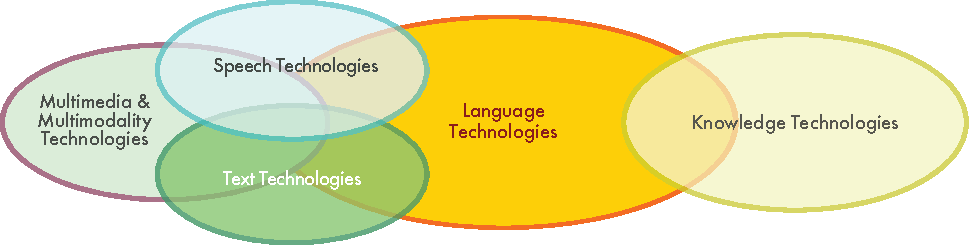
\includegraphics[width=\textwidth]{../_media/english/language_technologies}
  \caption{Language technologies}
  \label{fig:ltincontext_en}
  \colorrule{grey3}{\textwidth}{1.5pt}
\end{figure*}

When we communicate, we combine language with other modes of communication and information media – for example speaking can involve gestures and facial expressions. Digital texts link to pictures and sounds. Movies may contain language in spoken and written form. In other words, speech and text technologies overlap and interact with other multimodal communication and multimedia technologies.

In this section, we will discuss the main application areas of language technology, i.\,e., language checking, web search, speech interaction, and machine translation. These applications and basic technologies include 

\begin{itemize}
\item spelling correction
\item authoring support
\item computer-assisted language learning
\item information retrieval 
\item information extraction
\item text summarisation
\item question answering
\item speech recognition 
\item speech synthesis 
\end{itemize}

\begin{figure*}[b]
  \colorrule{grey3}{\textwidth}{1.5pt}
  \center
  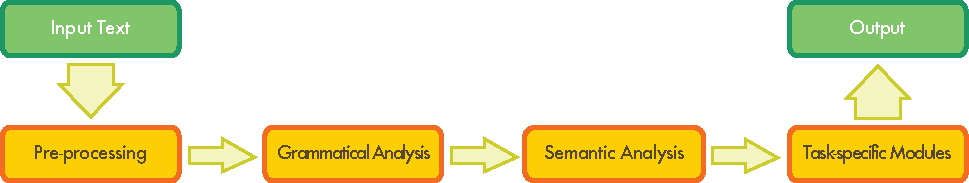
\includegraphics[width=\textwidth]{../_media/english/text_processing_app_architecture}
  \caption{A typical text processing architecture}
  \label{fig:textprocessingarch_en}
  \colorrule{grey3}{\textwidth}{1.5pt}
\end{figure*}

Language technology is an established area of research with an extensive set of introductory literature. The interested reader is referred to the following references:  \cite{jurafsky-martin01, manning-schuetze1, lt-survey1}.

Before discussing the above application areas, we will briefly describe the architecture of a typical LT system.

% --------------------------------------------------------------------------
 \subsection {Application Architectures}
   
 
Software applications for language processing typically consist of several components that mirror different aspects of language. Figure \ref{fig:textprocessingarch_en} shows a highly simplified architecture that can be found in a typical text processing system. The first three modules handle the structure and meaning of the text input:

\begin{enumerate}
 \item Pre-processing: cleans the data, analyses or removes formatting, and detects the input language. In Serbian it can also help in resolving the Latin and Cyrillic alphabets duality, as well as the Ekavian – Ijekavian duality.
\item Grammatical analysis: finds the verb, its objects, modifiers and other sentence elements; detects the sentence structure.
\item Semantic analysis: performs disambiguation (i.\,e.~computes the appropriate meaning of words in a given context); resolves anaphora (i.\,e.~which pronouns refer to which nouns in the sentence) and substitute expressions; represents the meaning of the sentence in a machine-readable way.
\end{enumerate}

After analysing the text, task-specific modules can perform other operations, such as automatic summarisation and database look-ups. This is a simplified and idealised description of the application architecture, and illustrates the complexity of LT applications. 

In the remainder of this section, we firstly introduce the core application areas for language technology, and follow this with a brief overview of the state of LT research and education today, and a description of past and present research programmes. Finally, we present an expert estimate of core LT tools and resources for Serbian in terms of various dimensions such as availability, maturity and quality. The general situation of LT for the Serbian language is summarised in
figure~\ref{tab:lrlttable} (p.~\pageref{tab:lrlttable}) at the end of this chapter. This table lists all tools and
resources that are boldfaced in the text. 
 

% --------------------------------------------------------------------------
 \subsection {Core Application Areas}
   
In this section, we focus on the most important LT tools and resources, and give an overview of LT activities in Serbia.   

% --------------------------------------------------------------------------
 \subsubsection {Language checking}
   
 Anyone who has used a word processor such as Microsoft Word knows that it has a spell checker that highlights spelling mistakes and proposes corrections. The first spelling correction programs compared a list of extracted words against a dictionary of correctly spelled words. Today these programs are far more sophisticated. Using language-dependent algorithms for \textbf{grammatical analysis}, they detect errors related to morphology (e.\,g.~plural formation) as well as syntax–related errors, such as a missing verb or a conflict of verb-subject agreement (e.\,g.~\textit{she *write a letter}). However, most spell checkers will not find any errors in the following text \cite{ZAR}:


\begin{quote}
 I have a spelling checker, \\
 It came with my PC. \\
 It plane lee marks four my revue \\
 Miss steaks aye can knot sea.  \\
\end{quote}

\vspace{-0.5cm}

Handling these kinds of errors usually requires an analysis of the context. For example, whether a word needs to be capitalised in Serbian or not:

\begin{quote}
Divio se \textit{Ruži.} [He admired \textit{Rose}.]\\
Divio se \textit{ruži.} [He admired \textit{the rose}.]\\
\end{quote}
 
\vspace{-0.5cm}

This type of analysis either needs to draw on language-specific \textbf{grammars} laboriously coded into the software by experts, or on a statistical language model. In this case, a model calculates the probability of a particular word occuring in a specific position (e.\,g.~between the words that precede and follow it). For example, \textit{plava laguna} (blue lagoon) is a much more probable word sequence than \textit{plava Laguna} (where Laguna is the name of a publishing house). A statistical language model can be automatically created by using a large amount of (correct) language data, a \textbf{text corpus}. These two approaches have been mostly developed around English language data. Neither approach can be transferred easily to Serbian, because the language has a flexible word order and rich inflection.

\vspace{-0.5cm}
\boxtext{Language checking is not limited to word processors but also applies to authoring systems.}

The first attempts to develop spelling checking software for Serbian dates back to the end of the 1970s \cite{UROSEVIC}, motivated by problems confronted by large publishing houses. To date, free spelling checking modules for Serbian are available for OpenOffice \cite{OpenOffice} on different operating systems, and there exists also a custom-made product, the RAS package, \cite{RASPROG} developed by the Srbosof company (individualised installation).  
 
\begin{figure*}[htb]
  \colorrule{grey3}{\textwidth}{1.5pt}
  \center
  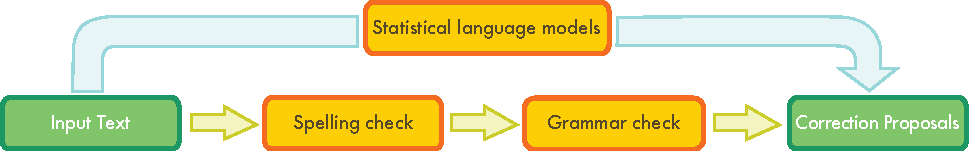
\includegraphics[width=\textwidth]{../_media/english/language_checking}
  \caption{Language checking (statistical; rule-based)}
  \label{fig:langcheckingaarch_en}
  \colorrule{grey3}{\textwidth}{1.5pt}
\end{figure*}

Language checking is not limited to word processors; it is also used in “authoring support systems”, i.\,e.~software environments in which manuals and other documentation are written to special standards for complex IT, healthcare, engineering and other products. To offset customer complaints about incorrect use and damage claims resulting from poorly understood instructions, companies are increasingly focusing on the quality of technical documentation while targeting the international market (via translation or localisation) at the same time. Advances in natural language processing have led to the development of authoring support software, which helps the writer of technical documentation to use vocabulary and sentence structures that are consistent with industry rules and (corporate) terminology restrictions. 


Besides spelling checkers and authoring support, language checking is also important in the field of computer-assisted language learning. And language checking applications also automatically correct search engine queries, as found in Google's \textit{Did you mean\ldots}  suggestions. 
 
% --------------------------------------------------------------------------
 \subsubsection {Web Search}
   

\begin{figure*}[htb]
  \colorrule{grey3}{\textwidth}{1.5pt}
  \center
  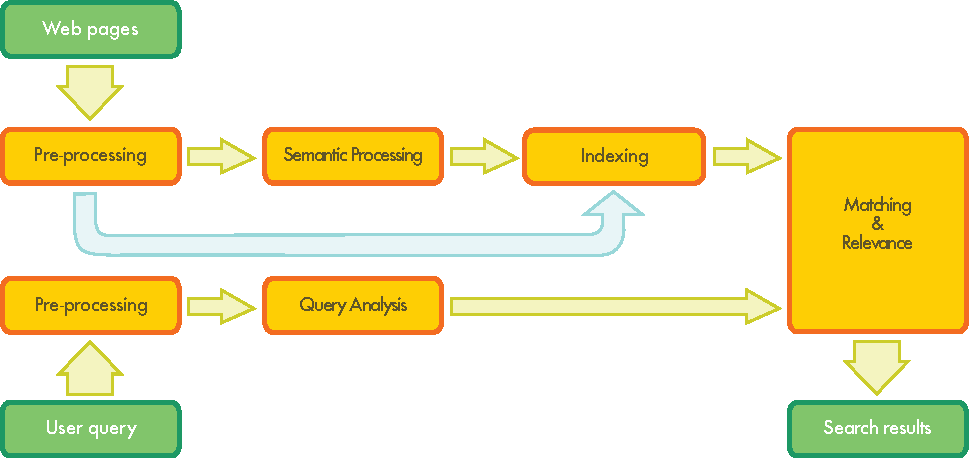
\includegraphics[width=\textwidth]{../_media/english/web_search_architecture}
  \caption{Web search}
  \label{fig:websearcharch_en}
  \colorrule{grey3}{\textwidth}{1.5pt}
 \end{figure*}


Searching the Web, intranets or digital libraries is probably the most widely used yet largely underdeveloped language technology application today. The Google search engine, which started in 1998, now handles about 80\% of all search queries. \cite{SPIEGEL} The verbs \textit{guglati/izguglati} are in common use in Serbian. The Google search interface and results page display has not significantly changed since the first version. However, in the current version, Google offers spelling correction for misspelled words and incorporates basic semantic search capabilities that can improve search accuracy by analysing the meaning of terms in a search query context \cite{PCWORLD}. The Google success story shows that a large volume of data and efficient indexing techniques can deliver satisfactory results using a statistical approach to language processing.

For more sophisticated information requests, it is essential to integrate deeper linguistic knowledge to facilitate text interpretation. Experiments using \textbf{lexical resources} such as machine-readable thesauri or ontological language resources (e.\,g.~WordNet for English or SrpNet for Serbian) have demonstrated improvements in finding pages using synonyms of the original search terms, such as \textit{atomska energija} (atomic energy) and \textit{nuklearna energija} (nuclear energy), or even more loosely related terms, such as \textit{beli luk} and \textit{češnjak} (synonyms for garlic).

\vspace{-0.5cm}
\boxtext{The next generation of search engines\\will have to include much more sophisticated language technology. }

The next generation of search engines will have to include much more sophisticated language technology, especially to deal with search queries consisting of a question or other sentence type rather than a list of keywords. For the query, \textit{Give me a list of all companies that were taken over by other companies in the last five years}, a syntactic as well as \textbf{semantic analysis} is required. The system also needs to provide an index to quickly retrieve relevant documents. A satisfactory answer will require syntactic parsing to analyse the grammatical structure of the sentence and determine that the user wants companies that have been acquired, rather than companies that have acquired other companies. For the expression \textit{last five years}, the system needs to determine the relevant range of years, taking into account the present year. The query then needs to be matched against a huge amount of unstructured data to find the pieces of information that are relevant to the user’s request. This process is called information retrieval, and involves searching and ranking relevant documents. To generate a list of companies, the system also needs to recognise a particular string of words in a document represents a company name, using a process called named entity recognition.


A more demanding challenge is matching a query in one language with documents in another language. Cross-lingual information retrieval involves automatically translating the query into all possible source languages and then translating the results back into the target language. 

Now that data is increasingly found in non-textual formats, there is a need for services that deliver multimedia information retrieval by searching images, audio files and video data. In the case of audio and video files, a speech recognition module must convert the speech content into text (or into a phonetic representation) that can then be matched against a user query.

Popular sites in Serbia offering search capabilities, such as B92 and Krstarica, mostly rely on Google services. \cite{ALEXA} An attempt to introduce a search engine which would perform exclusively a top-down search of the .rs domain, and which would partly be adjusted to the specific features of Serbian, was abandoned in 2010 as unprofitable. A certain number of SMEs is working on the enhancement of search services, albeit mainly for foreign partners and for English. 

For research purposes, experiments have been performed with query expansion, by sending queries expanded on the basis of morphological dictionaries and multilingual semantic networks to search engines. The experiments yielded interesting and useful results \cite{PAPINENI} in various domains.  

% --------------------------------------------------------------------------
 \subsubsection {Speech Interaction}
   

Speech interaction is one of many application areas that depend on speech technology, i.\,e.~technologies for processing spoken language. Speech interaction technology is used to create interfaces that enable users to interact in spoken language instead of a graphical display, keyboard and mouse. Today, these voice user interfaces (VUI) are used for partially or fully automated telephone services provided by companies to customers, employees or partners. Business domains that rely heavily on VUIs include banking, supply chain, public transportation, and telecommunications. Other uses of speech interaction technology include interfaces to car navigation systems and the use of spoken language as an alternative to the graphical or touch-screen interfaces in smartphones. Speech interaction technology comprises four technologies: 

\begin{figure*}[htb]
  \colorrule{grey3}{\textwidth}{1.5pt}
  \center
  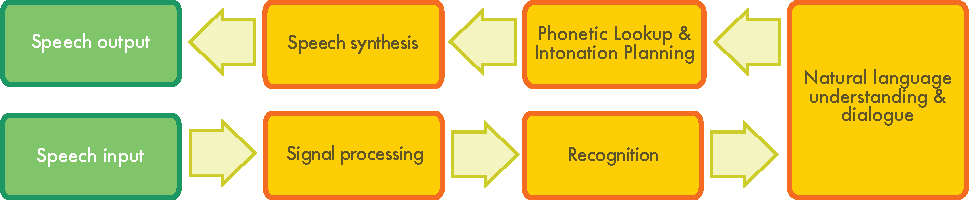
\includegraphics[width=\textwidth]{../_media/english/simple_speech-based_dialogue_architecture}
  \caption{Speech-based dialogue system}
  \label{fig:dialoguearch_en}
  \colorrule{grey3}{\textwidth}{1.5pt}
\end{figure*}


\begin{enumerate}
\item Automatic \textbf{speech recognition} (ASR) determines which words are actually spoken in a given sequence of sounds uttered by a user.
\item Natural language understanding analyses the syntactic structure of a user’s utterance and interprets it according to the system in question.
\item  Dialogue management determines which action to take given the user input and system functionality.
\item \textbf{Speech synthesis} (text-to-speech or TTS) transforms the system’s reply into sounds for the user. 
\end{enumerate}
One of the major challenges of ASR systems is to accurately recognise the words a user utters. This means restricting the range of possible user utterances to a limited set of keywords, or manually creating language models that cover a large range of natural language utterances. Using machine learning techniques, language models can also be generated automatically from \textbf{speech corpora}, i.\,e.~large collections of speech audio files and text transcriptions. Restricting utterances usually forces people to use the voice user interface in a rigid way and can damage user acceptance; but the creation, tuning and maintenance of rich language models will significantly increase costs. VUIs that employ language models and initially allow a user to express their intent more flexibly — prompted by a \textit{How may I help you?} greeting — tend to be automated and are better accepted by users. 

\boxtext{Speech interaction is the basis for interfaces that allow a user to interact with spoken language.}

Companies tend to use utterances pre-recorded by professional speakers for generating the output of the voice user interface. For static utterances where the wording does not depend on particular contexts of use or personal user data, this can deliver a rich user experience. But more dynamic content in an utterance may suffer from unnatural intonation because different parts of audio files have simply been strung together. Today’s TTS systems are getting better (though they can still be optimised) at producing natural-sounding dynamic utterances.  


Interfaces in speech interaction have been considerably standardised during the last decade in terms of their various technological components. There has also been strong market consolidation in speech recognition and speech synthesis. The national markets in the G20 countries (economically resilient countries with high populations) have been dominated by just five global players, with Nuance (USA) and Loquendo (Italy) being the most prominent players in Europe. In 2011, Nuance announced the acquisition of Loquendo, which represents a further step in market consolidation.

The speech synthesis and recognition methods in Serbia (and in the countries of the former Yugoslavia) were developed mainly in electrical engineering environments in cooperation with phonetics experts. These early endeavours were focused on recognition of isolated phonemes. A substantial breakthrough in this area was made by a group from the Faculty of Technical Sciences at the University of Novi Sad, when they developed, in addition to speech databases, a lexical database with more than 4,000,000 accentuated word forms for Serbian and more than 3,000,000 word forms for Croatian. Various applications in the fields of TTS and ASR have been developed based on these resources. Serbian speech recognition and generation has been commercialised by the AlfaNum company, a spin-off of the University of Novi Sad. This company is successfully conducting business activities in other countries of the former Yugoslavia as well (Croatia, Macedonia, Bosnia and Montenegro). The AlfaNum company has a considerable number of users among Serbian companies. 

When translating to Serbian, Google translator also offers an elementary TTS for translation results (albeit without built-in accents).


Looking ahead, there will be significant changes, due to the spread of smartphones as a new platform for managing customer relationships, in addition to fixed telephones, the Internet and e-mail. This will also affect how speech interaction technology is used. In the long term, there will be fewer telephone-based VUIs, and spoken language apps will play a far more central role as a user-friendly input for smartphones. This will be largely driven by stepwise improvements in the accuracy of speaker-independent speech recognition via the speech dictation services already offered as centralised services to smartphone users.

% --------------------------------------------------------------------------
 \subsubsection {Machine translation}

\begin{figure*}[htb]
  \colorrule{grey3}{\textwidth}{1.5pt}
  \center
  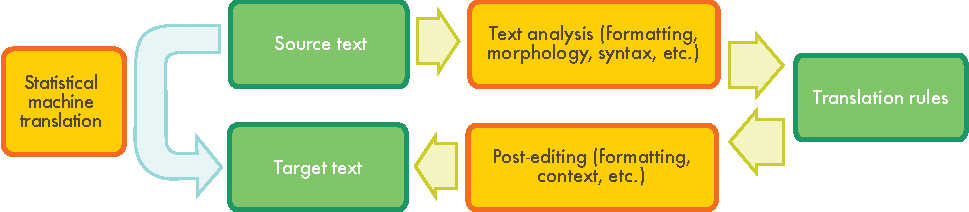
\includegraphics[width=\textwidth]{../_media/english/machine_translation}
  \caption{Machine translation (statistical; rule-based)}
  \label{fig:mtarch_en}
  \colorrule{grey3}{\textwidth}{1.5pt}
\end{figure*}
 


The idea of using digital computers to translate natural languages can be traced back to 1946 and was followed by substantial funding for research during the 1950s and again in the 1980s. Yet \textbf{machine translation} (MT) still cannot deliver on its initial promise of providing across-the-board automated translation.

\boxtext{At its basic level, Machine Translation simply substitutes words in one natural language with words in another language.}

The most basic approach to machine translation is the automatic replacement of the words in a text written in one natural language with the equivalent words of another language. This can be useful in subject domains that have a very restricted, formulaic language such as weather reports.  However, in order to produce a good translation of less restricted texts, larger text units (phrases, sentences, or even whole passages) need to be matched to their closest counterparts in the target language. The major difficulty is that human language is ambiguous. Ambiguity creates challenges on multiple levels, such as word sense disambiguation at the lexical level (a \textit{jaguar} is a brand of car or an animal) or the assignment of case on the syntactic level, for example:

\begin{itemize}
\item \textit{Policajac je uspeo da primeti čoveka bez dvogleda.} (The policeman caught sight of the man without binocular.)
\item \textit{Policajac je uspeo da primeti čoveka bez revolvera.} (The policeman caught sight of the man without the revolver.)
\end{itemize}


One way to build an MT system is to use linguistic rules. For translations between closely related languages, a translation using direct substitution may be feasible in cases such as the above example. However, rule-based (or linguistic knowledge-driven) systems often analyse the input text and create an intermediary symbolic representation from which the target language text can be generated. The success of these methods is highly dependent on the availability of extensive lexicons with morphological, syntactic, and semantic information, and large sets of grammar rules carefully designed by skilled linguists. This is a very long and therefore costly process.

In the late 1980s when computational power increased and became cheaper, interest in statistical models for machine translation began to grow. Statistical models are derived from analysing bilingual text corpora, \textbf{parallel corpora}, such as the Europarl parallel corpus, which contains the proceedings of the European Parliament in 21 European languages. Given enough data, statistical MT works well enough to derive an approximate meaning of a foreign language text by processing parallel versions and finding plausible patterns of words. Unlike knowledge-driven systems, however, statistical (or data-driven) MT systems often generate ungrammatical output. Data-driven MT is advantageous because less human effort is required, and it can also cover special particularities of the language (e.\,g.~idiomatic expressions) that are often ignored in knowledge-driven systems. 

The strengths and weaknesses of knowledge-driven and data-driven machine translation tend to be complementary, so that nowadays researchers focus on hybrid approaches that combine both methodologies. One such approach uses both knowledge-driven and data-driven systems, together with a selection module that decides on the best output for each sentence. However, results for sentences longer than, say, 12 words, will often be far from perfect. A more effective solution is to combine the best parts of each sentence from multiple outputs; this can be fairly complex, as corresponding parts of multiple alternatives are not always obvious and need to be aligned. 


\boxtext{Machine translation is particularly challenging for the Serbian language. }

When it comes to the relation between Serbian and other foreign languages, the problems depend on the nature of the specific language (whether its morphology is developed or not, whether it has a free or fixed distribution of sentence constituents, whether it possesses an article or not, whether it is written in the Cyrillic or Latin alphabet, whether it uses logical or grammatical punctuation, etc.) However, there is not only an issue of problems here, but also of possibilities for cooperation in solving similar problems. In that sense, cooperation with projects related to computational processing of other Slavonic languages is especially useful. However, lexical-terminological relations are also important, namely, the extent to which a foreign language has influenced the elaboration of Serbian. In this field, cooperation should be sought with projects aimed at computational processing of languages which have served and are still serving as the backbone for the elaboration of Serbian, notably, English, French, German and Russian.

It should also be added that contrastive research on the relation between Serbian and some foreign languages is also taking place. However, there is unfortunately insufficient cooperation between linguists dealing with Serbian as mother tongue and those who engage in contrastive research as experts for foreign languages. Another problem is the insufficient number of large bilingual dictionaries. 

The greatest need for LT in Serbia is in the area of translation. There are some specialised associations (e.\,g.~the Association of Literary Translators of Serbia, the Association of Technical and Scientific of Serbia), some local SMEs (e.\,g.~Elitence and Proverbum) and some foreign companies (e.\,g.~WorldLingo) that offer professional translation services or free, phrase-based machine translation (e.\,g.~Google Translate, WorldLingo). Some of them use proprietary electronic dictionaries in their work, while WorldLingo also offers enhanced machine translation services (web sites, texts, documents, emails, APIs, etc.).

Apart from the well-known freely available Google statistical translation systems which also include Serbian, no other MT systems have been produced for Serbian, with the exception of some preliminary work (e.\,g.~done as part of the SEE-ERA project) and toy experimental systems.

However, generic statistical MT systems such as Google Translate support Serbian to a considerable degree, especially in translation from and into English. Nevertheless, for other language pairs, the performance is low and the results far from comprehensible, sometimes even ridiculous. This is due to the scarcity of parallel corpora that are used to train statistical MT.

The quality of MT systems is still considered to have huge improvement potential. Challenges include the adaptability of the language resources to a given subject domain or user area and the integration into existing workflows with term bases and translation memories. 

Evaluation campaigns help compare the quality of MT systems, the different approaches and the status of the systems for different language pairs. Figure~\ref{fig:euromatrix} (p. ~\pageref{fig:euromatrix}), which was prepared in the course of the EC Euromatrix+ project, shows the pair-wise performances obtained for 22 of the 23 official EU languages (Irish was not compared). The results are ranked according to a BLEU score, which indicates higher scores for better translations. \cite{PAPINENI}  A human translator would achieve a score of around 80 points.

The best results (in green and blue) were achieved by languages that benefit from a considerable research effort in coordinated programs and from the existence of many parallel corpora (e.\,g.~English, French, Dutch, Spanish and German). Languages with poorer results are shown in red. These languages either lack such development efforts or are structurally very different from other languages (e.\,g.~Hungarian, Maltese and Finnish).


% --------------------------------------------------------------------------
 \subsection {Other Application Areas}

Building language technology applications involves a range of subtasks that do not always surface at the level of interaction with the user, but they provide significant service functionalities “behind the scenes” of the system in question. They all form important research issues that have now evolved into individual sub-disciplines of computational linguistics. Question answering, for example, is an active area of research for which annotated corpora have been built and scientific competitions have been initiated. The concept of question answering goes beyond keyword-based searches (in which the search engine responds by delivering a collection of potentially relevant documents) and enables users to ask a concrete question to which the system provides a single answer. For example:

\begin{itemize}
\item[] \textit{Question: How old was Neil Armstrong when he stepped on the moon?}
\item[] \textit{Answer: 38.}
\end{itemize}


While question answering is obviously related to the core area of web search, it is nowadays an umbrella term for such research issues as which different types of questions exist, and how they should be handled; how a set of documents that potentially contain the answer can be analysed and compared (do they provide conflicting answers?); and how specific information (the answer) can be reliably extracted from a document without ignoring the context.    


Question answering is in turn related to information extraction (IE), an area that was extremely popular and influential when computational linguistics took a statistical turn in the early 1990s. IE aims to identify specific pieces of information in specific classes of documents, such as the key players in company takeovers as reported in newspaper stories. Another common scenario that has been studied is reports on terrorist incidents. The task here consists of mapping appropriate parts of the text to a template that specifies the perpetrator, target, time, location and results of the incident. Domain-specific template-filling is the central characteristic of IE, which makes it another example of a “behind the scenes” technology that forms a well-demarcated research area, which in practice needs to be embedded into a suitable application environment.

\boxtext{Language technology applications often provide significant service functionalities behind the scenes of larger software systems. }


Text summarisation and \textbf{text generation} are two borderline areas that can act either as standalone applications or play a supporting role. Summarisation attempts to give the essentials of a long text in a short form, and is one of the features available in Microsoft Word. It mostly uses a statistical approach to identify the “important” words in a text (i.\,e., words that occur very frequently in the text in question but less frequently in general language use) and determine which sentences contain the most of these “important” words. These sentences are then extracted and put together to create the summary. In this very common commercial scenario, summarisation is simply a form of sentence extraction, and the text is reduced to a subset of its sentences. An alternative approach, for which some research has been carried out, is to generate brand new sentences that do not exist in the source text. This requires a deeper understanding of the text, which means that so far this approach is far less robust. On the whole, a text generator is rarely used as a stand-alone application but is embedded into a larger software environment, such as a clinical information system that collects, stores and processes patient data. Creating reports is just one of many applications for text summarisation.


Within the aforementioned areas, highly successful experiments for Serbian are underway related to named entity extraction as a part of the information extraction problem. A speedy development of IE and QA is expected, given the extent of developed morphological dictionaries and local grammars.

There are other fields in which linguistic technology is being applied. One of them is plagiarism detection, which uses language-independent technologies, but may be enhanced with search for simple paraphrases of the text. A research along these lines for scientific articles in Serbian has been realised by the CEON company. \cite{CEON}

% --------------------------------------------------------------------------
 \subsection {Educational Programmes}

Language Technology is a highly interdisciplinary field, involving the expertise of linguists, computer scientists, mathematicians, philosophers, psycholinguists, and neuroscientists, among others. As a result, it has not yet acquired a fixed place in the Serbian higher education system and is largely limited to isolated courses within more general post-graduate study programmes. Paradoxically, despite this state of affairs, short research seminars on topics related to computational linguistics for high school students are organised within the Petnica science centre \cite{PETNICA} each year. 

At the level of university studies, topics from the field of computational linguistics are present within computer science, electronics, library science, linguistics and psychology studies at the Universities of Belgrade and Novi Sad. Courses offered to students cover the basic concepts of natural language processing, but they aim to educate students for other professions. As part of undergraduate studies at the Faculty of Mathematics in Belgrade, courses in lexical analysis and text mining are offered, in addition to courses providing basic mathematical knowledge necessary in the field of natural language processing (especially statistics, algebra, and logic), whereas a greater choice of courses in the HLT field exist at the level of doctoral studies. The most comprehensive education in the HLT field is offered to students at the Department of Library Science at the Faculty of Philology, whereas at other departments students take at most one introductory course. Within Serbian language studies, education in the field of NLP is not envisaged. The Faculties of Philosophy in Belgrade and Novi Sad offer courses in psycholinguistics, where students can get acquainted with methods of statistical text processing. Methods of interest for speech processing are studied at technical faculties. None of the faculties offer a curriculum giving expertise in the field of computational linguistics or language technologies. 
 

% --------------------------------------------------------------------------
 \subsection {National Projects and Efforts}

Due to various reasons the LT industry in Serbia is relatively undeveloped compared to the leading EU economies. The main driving force behind the development of LT in Serbia are mainly domestic SMEs but also some foreign companies, which sometimes provide support for the Serbian language in various LT-related applications. Since a national programme to support the development of language technologies does not exist, their development and application are often realised in an uncoordinated manner. The introduction of language technologies in Serbia follows at least three different directions: (a) through state supported scientific and technology development projects (b) through (mainly) foreign companies which, in addition to computer equipment, also offer some sort of language support, and (c) through in-house development within domestic organisations such as publishing houses and translation agencies. Except in rare cases, these three lines of activities are realised independently from each other. 

On the other hand, the computer-literate population in Serbia is accustomed to using English GUIs even though some of them may not speak English. They often find the localised versions awkward and imprecise, so they are reluctant to use them. The only applications that massively use Serbian GUI are various business, financial and accountant applications including the SAP ERP system. However, there are also some examples of GUI localised by other renowned software vendors like Microsoft (e.\,g.~MS Windows, MS Office), Google or Oracle (localisation of OpenOffice, funded in the 2008-- 2011 period by the Ministry for Telecommunications and Information Society through a project at the Faculty of Mathematics \cite{OO_MATF}).

Interdisciplinarity has been recognised only in the latest cycle of scientific projects (for the 2011-2014 period) funded by the Ministry of Education and Science. Until 2010 scientific projects (and hence criteria for their evaluation) have been strictly divided among the fields of mathematics (including computer science as its part), language, and technological disciplines. In such a setting, it was hard to realise the natural combination of disciplines which form the basis of language technology development. In this context, it was necessary to establish connections between research in the field of Serbian language and informatics. 

The first project along these lines entitled “Interactions between text and dictionaries” was conceived in 2002 as a joint project of the Departments of Serbian at the Faculty of Philology in Belgrade and the Faculty of Philosophy in Novi Sad, as well as the Faculty of Mathematics in Belgrade. In the scope of this project, the first corpus of contemporary Serbian was developed, \cite{KORPUS} accessible via the web, currently having more than 300 registered users from different Serbian and foreign universities and institutes. Development of an electronic morphological dictionary of Serbian following the so-called LADL format was also initiated within the scope of this project. \cite{KRSTEV} The project was later continued as a joint project of the Department of Serbian at the Faculty of Philology and the Faculty of Mathematics in the period from 2006 to 2010 under the name “A theoretical and methodological framework for the modernisation of Serbian” and from 2011 to 2014 under the name “Serbian and its resources: theory, description and applications”. Within the scope of these projects, the development of the electronic dictionary of simple words was finalised, the development of a dictionary of compounds was initiated. Aligned French-Serbian and English-Serbian corpora of literary texts were developed, as well as local grammars for certain segments of Serbian (especially for named entities). Different software tools were also developed, among which special attention should be given to LeXimir, a workstation which enables integration and transformation of heterogeneous lexical resources.
 
Parallel with this research in the field of language, a project was funded within the social sciences field under the name “Fundamental cognitive processes and functions”, realised by the Department of Psychology at the Faculty of Philosophy in Belgrade. The aim of this project, among other things, was to investigate the possibility of the automatic annotation of texts based on an annotated corpus, \cite{SRB_KORPUS} developed during the 1950s and converted to electronic form in the 1990s. 

Speech synthesis and recognition is being realised at the Faculty of Technical Sciences of the University of Novi Sad through projects of technological development from 2005, namely “Development of speech technologies in Serbian and their application in Telekom Serbia” (2005-2007), “Man-machine speech communication” (2008-2010), “Development of dialogue systems for Serbian and other South-Slavic languages” (2011--2014). They provide support for different TTS and ASR applications and services including IVR systems, private branch exchanges, call centres, audio logging, track commercials, word spotter, etc.
 
Other single resources of interest for HLT have been developed within other scientific areas, albeit without any direct interaction with the aforementioned projects. Let us just mention a few examples such as the Serbian-English geological thesaurus \cite{RGF} and the folkloristic database DABI of the Institute of Balkan studies SASA. \cite{BALKANINSTITUT} 

In addition to national projects, Serbian scientific institutions have also taken part in various international projects related to the HLT field. A certain level of activities was maintained during the UN sanctions due to the participation in projects TELRI I and II. \cite{TELRI} Although Serbian research groups could not participate at that time in the project MULTEXT-East \cite{NL}, they nevertheless produced useful resources in formats defined by that project: a morphosyntactic description of Serbian, an aligned version of the Serbian translation of Orwell’s \textit{1984}, its lemmatised morphosyntactically tagged version and a comprehensive dictionary covering \textit{1984}'s lexicon. 

\vspace{0.5cm}
\boxtext{The situation in various domains related to processing of Serbian differs, but there is definitely a considerable improvement in corpus development, morphological analysis, electronic dictionaries as well as NE extraction (dates, toponyms, etc.).}

After the sanctions were lifted, of particular importance was the BalkaNet \cite{CORDIS} project which enabled the development of a WordNet type semantic network for Serbian. The Serbian part of the multilingual lexical database of proper names Prolex \cite{CNRTL} was developed within the scope of bilateral cooperation with France, whereas a one-million aligned English-Serbian project, lemmatised and morphologically annotated, was developed within the scope of the Intera project.  This corpus was used for tagger training, as well as for experiments in alignment at the word level and in automatic translation.
 
Serbian participants were also involved in two regional projects. One of them was the SEE-ERA.NET - Building Language Resources and Translation Models for Machine Translation focused on South Slavic and Balkan Languages (ICT 10503 RP, 2007--2008). Its main contribution was the development of unidirectional translation models that rely on large-scale multilingual resources, namely \textit{The Acquis Communautaire}. However, since documents that are the base of this resource had not yet been translated into Serbian at that time no translation model was produced for Serbian. Translation of EU legislation is underway, and part of the translated material is already available. \cite{PREVODJENJE} For its part, the Serbian team contributed by developing another multilingual aligned resource based on Verne’s novel \textit{Around the World in 80 Days} (in 16 languages at that time).  The other project was WISE - An Electronic Marketplace to Support Pairs of Less Widely Studied European Languages (BSEC 009 / 05.2007, 2007 - 2008) with the aim not only to produce cross-lingual lexical resources enriched with linguistic meta-data but also to develop and promote an electronic marketplace for the less widely studied Balkan languages, including Serbian.

Further activities encompass, in the first place, the development of procedures for the syntactic analysis of Serbian, which, due to the free order of words and morphological richness, represents an extremely complex task. This means that new resources need to be developed, above all, new types of dictionaries and corpora, as well as accompanying tools.  


% --------------------------------------------------------------------------
 \subsection {Availability of Tools and Resources}
   
 
Table \ref{tab:lrlttable} summarises the current state of language technology support for the Serbian language. The rating for existing tools and resources was generated by leading experts in the field who provided estimates based on a scale from 0 (very low) to 6 (very high) according to seven criteria.

% Begin table
\begin{table*}[ht]
\centering

\begin{tabular}{>{\columncolor{orange1}}p{.33\linewidth}@{\hspace*{6mm}}c@{\hspace*{6mm}}c@{\hspace*{6mm}}c@{\hspace*{6mm}}c@{\hspace*{6mm}}c@{\hspace*{6mm}}c@{\hspace*{6mm}}c}
\rowcolor{orange1}
 \cellcolor{white}&
 \begin{sideways}\makecell[l]{Quantity}\end{sideways} &
 \begin{sideways}\makecell[l]{\makecell[l]{Availability} }\end{sideways} &
 \begin{sideways}\makecell[l]{Quality}\end{sideways} &
 \begin{sideways}\makecell[l]{Coverage}\end{sideways} &
 \begin{sideways}\makecell[l]{Maturity}\end{sideways} &
 \begin{sideways}\makecell[l]{Sustainability}\end{sideways} &
 \begin{sideways}\makecell[l]{Adaptability}\end{sideways} \\ \addlinespace

\multicolumn{8}{>{\columncolor{orange2}}l}{\textcolor{black}{Language Technology (Tools, Technologies and Applications)}} \\ \addlinespace

Speech Recognition	&2&2&1&1&1&1&0 \\ \addlinespace
Speech Synthesis &2&2&4&4&5&5&1\\ \addlinespace
Grammatical analysis &1&1&2,5&2&2&1,5&1,5\\ \addlinespace
Semantic analysis &1&1&1&1,5&1&1&1,5\\ \addlinespace
Language generation &0&0&0&0&0&0&0\\ \addlinespace
Machine translation &1&1&0&1&0&1&1\\ \addlinespace

\multicolumn{8}{>{\columncolor{orange2}}l}{\textcolor{black}{Language Resources (Resources, Data and Knowledge Bases)}} \\ \addlinespace

Text corpora &0,5&1&0,5&1&1&1&0,5\\ \addlinespace
Speech corpora &1&2&4&4&3&3&3\\ \addlinespace
Parallel corpora &3&3&3&2&2&2&3\\ \addlinespace
Lexical resources &1&2&2&2&2&2&2,5\\ \addlinespace
Grammars &1&1&0&1&0&1&1\\
\end{tabular}
\caption{State of language technology support for Serbian}
\label{tab:lrlttable}
\end{table*}



For Serbian, the state of resources and technologies could be described as follows:
\begin{itemize}
\item Where morphological issues and issues related to them are concerned, it is safe to say that the level of development of technologies and resources is satisfactory, mainly due to the existence of large electronic dictionaries and local grammars. An immediate consequence of this fact is that necessary tools for information retrieval and information extraction are available. Some of the dictionaries are ready for wider use, whereas some need to be upgraded, as for example SrpNet.
\item A reference corpus of contemporary Serbian in Ekavian dialect is available, as well as several parallel aligned corpora, all of which are available to researchers of Serbian. Current research is focused on upgrading the reference corpus and expanding it with the Ijekavian variant.
\item Speech technologies are well developed, and they have found wide use in business, but research needs to be further expanded, in order to expand the area of their usability.
\item Software aimed at enhancing the productivity of lexicographical work has been developed, but the issue of accepting new technologies in traditionally oriented lexicographic environments is an impediment to the speedier development of lexicography.
\item Successful experiments have been performed in some areas, such as shallow parsing, summarisation, machine translation, ontological resources, in a strictly research environment. However, the results obtained are still far from the level of development reached for developed European languages. The attention of researchers is also drawn to multimedia and multimodal documents, especially in the context of the digitisation of cultural heritage.
\end{itemize}
Given the complexity of Serbian syntax, areas based on deep parsing simply do not exist: sentence semantics, text semantics, and language generation. This results in the absence of a formalised syntax of Serbian and restricts the development of syntactically and semantically annotated corpora. The formalisation of Serbian syntax is thus the most urgent task for the further expansion of HLT. 
 


% --------------------------------------------------------------------------
 \subsection {Cross-language comparison}
   
The current state of LT support varies considerably from one language community to another. In order to compare the situation between languages, this section will present an evaluation based on two sample application areas (machine translation and speech processing) and one underlying technology (text analysis), as well as basic resources needed for building LT applications. 
The languages were clustered using the following five-point scale: 

    \begin{itemize}
      \item Excellent LT support
      \item Good support
      \item Moderate support
      \item Fragmentary support 
      \item Weak or no support
    \end{itemize}

LT support was measured according to the following criteria:
\begin{itemize}
\item Speech Processing: Quality of existing speech recognition technologies, quality of existing speech synthesis technologies, coverage of domains, number and size of existing speech corpora, amount and variety of available speech-based applications
\item Machine Translation: Quality of existing MT technologies, number of language pairs covered, coverage of linguistic phenomena and domains, quality and size of existing parallel corpora, amount and variety of available MT applications
\item Text Analysis: Quality and coverage of existing text analysis technologies (morphology, syntax, semantics), coverage of linguistic phenomena and domains, amount and variety of available applications, quality and size of existing (annotated) text corpora, quality and coverage of existing lexical resources (e.\,g.~WordNet) and grammars
\item Resources: Quality and size of existing text corpora, speech corpora and parallel corpora, quality and coverage of existing lexical resources and grammars
\end{itemize} 




The relevant tables show that the tools and resources available for Serbian are mostly in the bottom cluster. Serbian compares well with other languages with a small number of speakers, such as Croatian, Slovenian and Slovak but these languages lag far behind more widely spoken European languages such as German and French. However, even for the latter languages LT resources and tools clearly do not yet reach the quality and coverage of comparable resources and tools for English, which is in the lead in all LT areas. And there are still plenty of gaps in English language resources with regard to high quality applications.


% --------------------------------------------------------------------------
 \subsection {Conclusions}
   
\emph{In this series of white papers, we have provided the first high-level comparison of language technology support across 30 European languages.
By identifying the gaps, needs and deficits, the European language technology community and its related stakeholders are now in a position to design a large scale research and development programme aimed at building truly multilingual, technology-enabled communication across Europe.}

The results of this white paper series show that there is a dramatic difference in language technology support between  European languages. While there are good quality software and resources available for some languages and application areas, other (usually smaller) languages have substantial gaps. Many languages lack basic technologies for text analysis and the essential resources. 

Others have basic tools and resources, but there is little chance of implementing semantic methods in the near future. This means that a large-scale effort is needed to reach the ambitious goal of providing support for all European languages, for example through high quality machine translation.

The scope of the resources and the range of tools available for Serbian are still very limited, especially when compared to the resources and tools for languages like French, German, and especially English, and they are not sufficient in quality and quantity to develop the kind of technologies required to support a truly multilingual knowledge-based society. 

Technologies already developed and optimised for English cannot be simply transferred to handle Serbian. English-based systems for syntactic analysis of sentence structure are in general unsuitable for Serbian texts. The work on language processing for Serbian has been concentrated so far on the development of resources and tools that comply with the specific features of Serbian (in the first place a description of its rich morphology). This line of development should by all means be followed in the future. 

For a rather modest language community and research environment such as the Serbian one, cooperation both on the national and international level in developing language resources is of vital importance. This is true in general for the majority of Slavic languages, and this cooperation asks for further stimulative measures. There are especially great possibilities for cooperation among projects related to standard languages of Štokavian origin, as well as Slavic languages in general, given the common specific features shared among them. 

Serbia’s participation in CESAR and META-NET is expected to contribute to the development, standardisation and availability of several important LT resources and thus to the development of language technology for Serbian. META-NET’s long-term goal is to introduce high-quality language technology for all languages in order to achieve political and economic unity through cultural diversity. The technology will help tear down existing barriers and build bridges between Europe’s languages. This requires all stakeholders - in politics, research, business, and society - to unite their efforts for the future.

The Serbian language technology industry is extremely modest. There are just a few SMEs involved and their approach is basically founded on the application of “brute force”, which means that they are basically ignoring the specific features of Serbian. Our findings show that the only alternative is to make a substantial effort to create LT resources for Serbian, and use them to drive forward research, innovation and development. The need for large amounts of data and the extreme complexity of language technology systems makes it vital to develop a new infrastructure and a more coherent research organisation to stimulate greater sharing and cooperation. Another key contribution would be the establishment of multidisciplinary studies related to language processing at the master and doctoral levels, which are currently not available.

We can therefore conclude that there is a desperate need for a large, coordinated initiative focused on overcoming the differences in language technology readiness for European languages as a whole.

 
\begin{table*}[ht]
\small
\centering
\begin{tabular}
{ % defines color for each column.
>{\columncolor{corange5}} p{.17\linewidth}@{\hspace{.027\linewidth}}
>{\columncolor{corange4}}p{.17\linewidth}@{\hspace{.027\linewidth}}
>{\columncolor{corange3}}p{.17\linewidth}@{\hspace{.027\linewidth}}
>{\columncolor{corange2}}p{.17\linewidth}@{\hspace{.027\linewidth}}
>{\columncolor{corange1}}p{.17\linewidth} 
}
\rowcolor{orange1} % redefines color for all columns in row 1

  \multicolumn{1}{>{\columncolor{white}}c@{\hspace{.040\linewidth}}}{\textbf{Excellent}} & 
  \multicolumn{1}{@{}>{\columncolor{white}}c@{\hspace{.040\linewidth}}}{\textbf{Good}} &
  \multicolumn{1}{@{}>{\columncolor{white}}c@{\hspace{.040\linewidth}}}{\textbf{Moderate}} &
  \multicolumn{1}{@{}>{\columncolor{white}}c@{\hspace{.040\linewidth}}}{\textbf{Fragmentary}} &
  \multicolumn{1}{@{}>{\columncolor{white}}c}{\textbf{Weak/no}} \\ 
  \multicolumn{1}{>{\columncolor{white}}c@{\hspace{.040\linewidth}}}{\textbf{support}} & 
  \multicolumn{1}{@{}>{\columncolor{white}}c@{\hspace{.040\linewidth}}}{\textbf{support}} &
  \multicolumn{1}{@{}>{\columncolor{white}}c@{\hspace{.040\linewidth}}}{\textbf{support}} &
  \multicolumn{1}{@{}>{\columncolor{white}}c@{\hspace{.040\linewidth}}}{\textbf{support}} &
  \multicolumn{1}{@{}>{\columncolor{white}}c}{\textbf{support}} \\ \addlinespace

& \vspace*{0.5mm}English
& \vspace*{0.5mm}German \newline   
Italian \newline  
Finnish \newline 
French \newline 
Dutch \newline 
Portuguese \newline 
Spanish \newline
Czech \newline 
& \vspace*{0.5mm}Basque \newline 
Bulgarian \newline 
Danish \newline 
Estonian \newline 
Galician\newline 
Greek \newline  
Irish \newline  
Catalan \newline 
Norwegian \newline 
Polish \newline 
Swedish \newline
\textbf{Serbian} \newline 
Slovak \newline 
Slovenian \newline 
Hungarian  \newline
& \vspace*{0.5mm}Icelandic \newline  
Croatian \newline 
Latvian \newline 
Lithuanian \newline 
Maltese \newline 
Romanian\\
\end{tabular}
\label{fig:speech_cluster}
\caption{Language clusters for speech processing}
\end{table*}

\begin{table*}[ht]
\small
\centering
\begin{tabular}
{ % defines color for each column.
>{\columncolor{corange5}} p{.17\linewidth}@{\hspace{.027\linewidth}}
>{\columncolor{corange4}}p{.17\linewidth}@{\hspace{.027\linewidth}}
>{\columncolor{corange3}}p{.17\linewidth}@{\hspace{.027\linewidth}}
>{\columncolor{corange2}}p{.17\linewidth}@{\hspace{.027\linewidth}}
>{\columncolor{corange1}}p{.17\linewidth} 
}
\rowcolor{orange1} % redefines color for all columns in row 1

  \multicolumn{1}{>{\columncolor{white}}c@{\hspace{.040\linewidth}}}{\textbf{Excellent}} & 
  \multicolumn{1}{@{}>{\columncolor{white}}c@{\hspace{.040\linewidth}}}{\textbf{Good}} &
  \multicolumn{1}{@{}>{\columncolor{white}}c@{\hspace{.040\linewidth}}}{\textbf{Moderate}} &
  \multicolumn{1}{@{}>{\columncolor{white}}c@{\hspace{.040\linewidth}}}{\textbf{Fragmentary}} &
  \multicolumn{1}{@{}>{\columncolor{white}}c}{\textbf{Weak/no}} \\ 
  \multicolumn{1}{>{\columncolor{white}}c@{\hspace{.040\linewidth}}}{\textbf{support}} & 
  \multicolumn{1}{@{}>{\columncolor{white}}c@{\hspace{.040\linewidth}}}{\textbf{support}} &
  \multicolumn{1}{@{}>{\columncolor{white}}c@{\hspace{.040\linewidth}}}{\textbf{support}} &
  \multicolumn{1}{@{}>{\columncolor{white}}c@{\hspace{.040\linewidth}}}{\textbf{support}} &
  \multicolumn{1}{@{}>{\columncolor{white}}c}{\textbf{support}} \\ \addlinespace
  
& \vspace*{0.5mm} English
& \vspace*{0.5mm} French \newline 
Spanish
& \vspace*{0.5mm}German \newline 
Italian \newline 
Catalan \newline 
Dutch \newline 
Polish \newline 
Romanian \newline 
Hungarian 
& \vspace*{0.5mm}Basque \newline 
Bulgarian \newline 
Danish \newline 
Estonian \newline 
Finnish \newline 
Galician \newline 
Greek \newline 
Irish \newline 
Icelandic \newline 
Croatian \newline 
Latvian \newline 
Lithuanian \newline 
Maltese \newline 
Norwegian \newline 
Portuguese \newline 
Swedish \newline 
\textbf{Serbian} \newline 
Slovak \newline 
Slovenian \newline 
Czech \newline
\end{tabular}
\label{fig:mt_cluster}
\caption{Language clusters for machine translation}
\end{table*}

\begin{table*}[ht]
  \small
  \centering
  \begin{tabular}
{ % defines color for each column.
>{\columncolor{corange5}} p{.17\linewidth}@{\hspace{.027\linewidth}}
>{\columncolor{corange3}}p{.17\linewidth}@{\hspace{.027\linewidth}}
>{\columncolor{corange3}}p{.17\linewidth}@{\hspace{.027\linewidth}}
>{\columncolor{corange2}}p{.17\linewidth}@{\hspace{.027\linewidth}}
>{\columncolor{corange1}}p{.17\linewidth} 
}
\rowcolor{orange1} % redefines color for all columns in row 1

  \multicolumn{1}{>{\columncolor{white}}c@{\hspace{.040\linewidth}}}{\textbf{Excellent}} & 
  \multicolumn{1}{@{}>{\columncolor{white}}c@{\hspace{.040\linewidth}}}{\textbf{Good}} &
  \multicolumn{1}{@{}>{\columncolor{white}}c@{\hspace{.040\linewidth}}}{\textbf{Moderate}} &
  \multicolumn{1}{@{}>{\columncolor{white}}c@{\hspace{.040\linewidth}}}{\textbf{Fragmentary}} &
  \multicolumn{1}{@{}>{\columncolor{white}}c}{\textbf{Weak/no}} \\ 
  \multicolumn{1}{>{\columncolor{white}}c@{\hspace{.040\linewidth}}}{\textbf{support}} & 
  \multicolumn{1}{@{}>{\columncolor{white}}c@{\hspace{.040\linewidth}}}{\textbf{support}} &
  \multicolumn{1}{@{}>{\columncolor{white}}c@{\hspace{.040\linewidth}}}{\textbf{support}} &
  \multicolumn{1}{@{}>{\columncolor{white}}c@{\hspace{.040\linewidth}}}{\textbf{support}} &
  \multicolumn{1}{@{}>{\columncolor{white}}c}{\textbf{support}} \\ \addlinespace
  
& \vspace*{0.5mm}English
& \vspace*{0.5mm}German \newline 
  French \newline 
  Italian \newline 
  Dutch \newline 
  Spanish 
& \vspace*{0.5mm}Basque \newline 
  Bulgarian \newline 
  Danish \newline 
  Finnish \newline 
  Galician \newline 
  Greek \newline 
  Catalan \newline 
  Norwegian \newline 
  Polish \newline 
  Portuguese \newline 
  Romanian \newline 
  Swedish \newline 
  Slovak \newline 
  Slovenian \newline 
  Czech \newline 
  Hungarian \newline 
& \vspace*{0.5mm}Estonian \newline 
  Irish \newline 
  Icelandic \newline 
  Croatian \newline 
  Latvian \newline 
  Lithuanian \newline 
  Maltese \newline 
  \textbf{Serbian} \\
  \end{tabular}
\label{fig:text_cluster}
\caption{Language clusters for text analysis}
\end{table*}

\begin{table*}[ht]
  \small
  \centering
\begin{tabular}
{ % defines color for each column.
>{\columncolor{corange5}} p{.17\linewidth}@{\hspace{.027\linewidth}}
>{\columncolor{corange4}}p{.17\linewidth}@{\hspace{.027\linewidth}}
>{\columncolor{corange3}}p{.17\linewidth}@{\hspace{.027\linewidth}}
>{\columncolor{corange2}}p{.17\linewidth}@{\hspace{.027\linewidth}}
>{\columncolor{corange1}}p{.17\linewidth} 
}
\rowcolor{orange1} % redefines color for all columns in row 1

  \multicolumn{1}{>{\columncolor{white}}c@{\hspace{.040\linewidth}}}{\textbf{Excellent}} & 
  \multicolumn{1}{@{}>{\columncolor{white}}c@{\hspace{.040\linewidth}}}{\textbf{Good}} &
  \multicolumn{1}{@{}>{\columncolor{white}}c@{\hspace{.040\linewidth}}}{\textbf{Moderate}} &
  \multicolumn{1}{@{}>{\columncolor{white}}c@{\hspace{.040\linewidth}}}{\textbf{Fragmentary}} &
  \multicolumn{1}{@{}>{\columncolor{white}}c}{\textbf{Weak/no}} \\ 
  \multicolumn{1}{>{\columncolor{white}}c@{\hspace{.040\linewidth}}}{\textbf{support}} & 
  \multicolumn{1}{@{}>{\columncolor{white}}c@{\hspace{.040\linewidth}}}{\textbf{support}} &
  \multicolumn{1}{@{}>{\columncolor{white}}c@{\hspace{.040\linewidth}}}{\textbf{support}} &
  \multicolumn{1}{@{}>{\columncolor{white}}c@{\hspace{.040\linewidth}}}{\textbf{support}} &
  \multicolumn{1}{@{}>{\columncolor{white}}c}{\textbf{support}} \\ \addlinespace
  
& \vspace*{0.5mm}English
& \vspace*{0.5mm}German \newline 
    French \newline 
    Dutch \newline 
    Swedish \newline 
    Czech \newline 
    Hungarian \newline
    Polish \newline
    Italian \newline
    Spanish
& \vspace*{0.5mm} Basque\newline 
    Bulgarian\newline 
    Danish \newline 
    Estonian \newline 
    Finnish \newline 
    Galician \newline 
    Greek \newline 
    Catalan \newline 
    Croatian \newline 
    Norwegian \newline 
    Portuguese \newline 
    Romanian \newline 
    \textbf{Serbian} \newline 
    Slovak \newline 
    Slovenian \newline
&  \vspace*{0.5mm} Irish \newline 
    Icelandic \newline 
    Latvian \newline 
    Lithuanian \newline 
    Maltese  \\
  \end{tabular}
  \label{fig:resources_cluster}
  \caption{Language clusters and resources}
\end{table*}


\end{multicols}

\clearpage


% --------------------------------------------------------------------------
\ssection[About META-NET]{About META-NET}

\begin{multicols}{2}

META-NET is a Network of Excellence partially funded by the European Commission \cite{rehm2011}. The network currently consists of 54 research centres in 33 European countries. META-NET forges META, the Multilingual Europe Technology Alliance, a growing community of language technology professionals and organisations in Eu-rope. META-NET fosters the technological foundations for a truly multilingual European information society that:

\begin{itemize}
\item makes communication and cooperation possible across languages;
\item grants all Europeans equal access to information and knowledge regardless of their language;
\item builds upon and advances functionalities of networked information technology.
\end{itemize}

The network supports a Europe that unites as a single digital market and information space. It stimulates and promotes multilingual technologies for all European languages. These technologies support automatic translation, content production, information processing and knowledge management for a wide variety of subject domains and applications. They also enable intuitive language-based interfaces to technology ranging from household electronics, machinery and vehicles to computers and robots.
Launched on 1 February 2010, META-NET has already conducted various activities in its three lines of action META-VISION, META-SHARE and META-RESEARCH.

\textbf{META-VISION} fosters a dynamic and influential stakeholder community that unites around a shared vision and a common strategic research agenda (SRA). The main focus of this activity is to build a coherent and cohesive LT community in Europe by bringing together representatives from highly fragmented and diverse groups of stakeholders. The present White Paper was prepared together with volumes for 29 other languages. The shared technology vision was developed in three sectorial Vision Groups. The META Technology Council was established in order to discuss and to prepare the SRA based on the vision in close interaction with the entire LT community.

\textbf{META-SHARE} creates an open, distributed facility for exchanging and sharing resources. The peer-to-peer network of repositories will contain language data, tools and web services that are documented with high-quality metadata and organised in standardised categories. The resources can be readily accessed and uniformly searched. The available resources include free, open source materials as well as restricted, commercially available, fee-based items.

\textbf{META-RESEARCH} builds bridges to related technology fields. This activity seeks to leverage advances in other fields and to capitalise on innovative research that can benefit language technology. In particular, the action line focuses on conducting leading-edge research in machine translation, collecting data, preparing data sets and organising language resources for evaluation purposes; compiling inventories of tools and methods; and organising workshops and training events for members of the community.\\\\

\textbf{\centerline{office@meta-net.eu -- http://www.meta-net.eu}}
\end{multicols}




\cleardoublepage

\appendix
\addtocontents{toc}{\protect\bigskip}

\bsection[Литература --- References]{Литература --- References}
\bibliographystyle{unsrt}
\bibliography{serbian_references}
  
\cleardoublepage

\bsection[Партнерске организације -- META-NET Members]{Партнерске организације --- META-NET Members}
\label{metanetmembers}

%  \small
%  \renewcommand{\arraystretch}{1.5}
%   \begin{longtable}{|p{2.5cm}|p{6.5cm}|p{4.5cm}|}
%  \arrayrulecolor{grey4}
%  \hline
%    \rowcolor{orange2} \textbf{Држава} & \textbf{Организација} & \textbf{Учесници} \\
%  \hline  
%  \hline
%  \rowcolor{corange1} Аустрија & Universität Wien & Gerhard Budin \\
%  \hline
%  \rowcolor{orange2} Белгија & Universiteit Antwerpen & Walter Daelemans \\
%  \hline
%  \rowcolor{corange1}  &Universitеit Leuven  & Dirk van Compernolle \\
%  \hline
%  \rowcolor{orange2} Бугарска & Българска академия на науките & Svetla Koeva \\
%  \hline
%  \rowcolor{corange1} Хрватска & Sveučilište u Zagrebu & Marko Tadić \\
%  \hline
%  \rowcolor{orange2} Кипар  & University of Cyprus  & Jack Burston \\
%  \hline
%  \rowcolor{corange1} Чешка република & Univerzita Karlova v Praze & Jan Hajic \\
%  \hline
%  \rowcolor{orange2} Данска & Københavns Universitet & Bente Maegaard, Bolette Sandford Pedersen \\
%  \hline
%  \rowcolor{corange1} Естонија & Tartu Ülikool & Tiit Roosmaa \\
%  \hline
%  \rowcolor{orange2} Финска  & Aalto University & Timo Honkela \\
%  \hline
%  \rowcolor{corange1} & Helsingin yliopisto & Kimmo Koskenniemi, Krister Linden \\
%  \hline
%  \rowcolor{orange2} Француска & Laboratoire d’Informatique pour la Mécanique et les Sciences de l’Ingénieur & Joseph Mariani \\
%  \hline
%  \rowcolor{corange1} & ELDA & Khalid Choukri \\
%  \hline
%  \rowcolor{orange2} Немачка & DFKI & Hans Uszkoreit and\newline Georg Rehm \\
%  \hline
%  \rowcolor{corange1} & RWTH Aachen\newline Saarland University & Hermann Ney\newline Manfred Pinkal \\
%  \hline
%  \rowcolor{orange2} Грчка  & Ινστιτούτο Επεξεργασίας του Λόγου* & Stelios Piperidis \\
%  \hline
%  \rowcolor{corange1} Мађарска &  Magyar Tudományos\newline Akadémia & TamásVáradi \\
%  \hline
%  \rowcolor{orange2} &  Budapesti Műszaki\newline és Gazdaságtudományi\newline Egyetem & Géza Németh,\newline GáborOlaszy \\
% \hline
%  \rowcolor{corange1} Исланд  & Háskóli Ísland s & Eiríkur Rögnvaldsson \\
%  \hline
%  \rowcolor{orange2} Ирска & Ollscoil Chathair\newline Bhaile Átha Cliath* & Josef van Genabith \\
%  \hline
%  \rowcolor{corange1} Италија & Consiglio Nazionale Ricerche,  Istituto di Linguistica Computazionale "Antonio Zampolli" & Nicoletta Calzolari \\
%  \hline
%  \rowcolor{orange2} & Fondazione Bruno Kessler & Bernardo Magnini \\
%  \hline
%  \rowcolor{corange1} Летонија & Tilde & Andrejs Vasiljevs \\
%  \hline
%  \rowcolor{orange2} &  Latvijas Universitāte & Inguna Skadina \\
%  \hline
%  \rowcolor{corange1} Литванија  & \cellcolor{corange1} Lietuvių kalbos institutas & \cellcolor{corange1}Jolanta Zabarskaitë \\
%  \hline
%  \rowcolor{orange2} Луксембург & Arax Ltd. & Vartkes Goetcherian \\
%  \hline
%  \rowcolor{corange1} Малта & L-Università ta' Malta & Mike Rosner \\
%  \hline
%  \rowcolor{orange2} Холандија & Universiteit Utrecht \newline University of Groningen & Jan Odijk \newline Gertjan van Noord \\
%  \hline
%  \rowcolor{corange1} Норвешка & Universitetet i Bergen & Koenraad De Smedt \\
%  \hline
%  \rowcolor{orange2} Пољска & Polska Akademia Nauk & Adam Przepiórkowski and Maciej Ogrodniczuk \\
%  \hline
%  \rowcolor{corange1} & Uniwersytet Łódzki & \cellcolor{corange1}Barbara Lewandowska-Tomaszczyk and Piotr Pęzik \\
%  \hline
%  \rowcolor{orange2} Португалија & Universidade de Lisboa & Antonio Branco \\
%  \hline
%  \rowcolor{corange1} & Institute for Systems Engineering and Computers & Isabel Trancoso \\
%  \hline
%  \rowcolor{orange2} Румунија & Academia Romana & Dan Tufis \\
%  \hline
%  \rowcolor{corange1} & Universitatea "Alexandru Ioan Cuza" & Dan Cristea \\
% \hline
%  \rowcolor{orange2} Србија & Универзитет у Београду & Duško Vitas, Cvetana Krstev, Ivan Obradović \\
%  \hline
%  \rowcolor{corange1} &  Институт ,,Михајло Пупин'' & Sanja Vraneš \\
%  \hline
%  \rowcolor{orange2} Словачка & Slovenská akadémia vied & Radovan Garabik \\
%  \hline
%  \rowcolor{corange1} Словенија & Institut "Jožef Stefan" & Marko Grobelnik \\
%  \hline
%  \rowcolor{orange2} Шпанија & Barcelona Media & Toni Badia \\
%  \hline
%  \rowcolor{corange1} & Universitat Politècnica de Catalunya & Asunción Moreno \\
%  \hline
%  \rowcolor{orange2} & Universitat Pompeu \newline Fabra &  Núria Bel\\
%  \hline
%  \rowcolor{corange1} Шведска &  Göteborgs universitet & Lars Borin \\
%  \hline
% \rowcolor{orange2} Уједињено краљевство & University of Manchester & Sophia Ananiadou \\
%  \hline
%  \rowcolor{orange2} &  University of Edinburgh & Steve Renals \\
%  \hline
%   \end{longtable}
%  \normalsize
%  \cleardoublepage


\small
\begin{longtable}{llp{105mm}}
  Аустрија & \textcolor{grey1}{Austria} & Zentrum für Translationswissenschaft, Universität Wien: Gerhard Budin\\ \addlinespace 
  Белгија & \textcolor{grey1}{Belgium} & Computational Linguistics and Psycholinguistics Research Centre, University of Antwerp: Walter Daelemans\\ \addlinespace
  & & Centre for Processing Speech and Images, University of Leuven: Dirk van Compernolle \\ \addlinespace
  Бугарска & \textcolor{grey1}{Bulgaria} & Institute for Bulgarian Language, Bulgarian Academy of Sciences: Svetla Koeva \\ \addlinespace
  Велика Британија & \textcolor{grey1}{UK} & 
  School of Computer Science, University of Manchester: Sophia Ananiadou \\ \addlinespace 
  & & Institute for Language, Cognition and Computation, Centre for Speech Technology Research, University of Edinburgh: Steve Renals \\ \addlinespace 
  & & Research Institute of Informatics and Language Processing, University of Wolverhampton: Ruslan Mitkov \\ \addlinespace 
  Грчка & \textcolor{grey1}{Greece} & R.C. “Athena”, Institute for Language and Speech Processing: Stelios Piperidis\\ \addlinespace  
  Данска &  \textcolor{grey1}{Denmark} & Centre for Language Technology, University of Copenhagen: \newline Bolette Sandford Pedersen, Bente Maegaard\\ \addlinespace
  Естонија & \textcolor{grey1}{Estonia} & Institute of Computer Science, University of Tartu: Tiit Roosmaa, Kadri Vider\\ \addlinespace
  Ирска & \textcolor{grey1}{Ireland} & School of Computing, Dublin City University: Josef van Genabith\\\addlinespace
  Исланд &  \textcolor{grey1}{Iceland} & School of Humanities, University of Iceland: Eiríkur Rögnvaldsson\\\addlinespace
  Италија & \textcolor{grey1}{Italy} & Consiglio Nazionale delle Ricerche, Istituto di Linguistica Computazionale “Antonio Zampolli”: Nicoletta Calzolari\\ \addlinespace
  & & Human Language Technology Research Unit, Fondazione Bruno Kessler:\newline Bernardo Magnini\\
  Кипар & \textcolor{grey1}{Cyprus} & Language Centre, School of Humanities: Jack Burston \\ \addlinespace
  Летонија & \textcolor{grey1}{Latvia} & Tilde: Andrejs Vasiļjevs\\ \addlinespace 
  & & Institute of Mathematics and Computer Science, University of Latvia: Inguna Skadiņa\\ \addlinespace
  Литванија &  \textcolor{grey1}{Lithuania} & Institute of the Lithuanian Language: Jolanta Zabarskaitė\\ \addlinespace
  Луксембург & \textcolor{grey1}{Luxembourg} & Arax Ltd.: Vartkes Goetcherian\\ \addlinespace
  Мађарска & \textcolor{grey1}{Hungary} & Research Institute for Linguistics, Hungarian Academy of Sciences: Tamás Váradi\\  \addlinespace
  & & Department of Telecommunications and Media Informatics, Budapest University of Technology and Economics: Géza Németh, Gábor Olaszy\\ \addlinespace
  Малта & \textcolor{grey1}{Malta} & Department Intelligent Computer Systems, University of Malta: Mike Rosner\\ \addlinespace
  Немачка & \textcolor{grey1}{Germany} & Language Technology Lab, DFKI: Hans Uszkoreit, Georg Rehm\\ \addlinespace
  & & Human Language Technology and Pattern Recognition, RWTH Aachen University: Hermann Ney \\ \addlinespace
  & & Department of Computational Linguistics, Saarland University: Manfred Pinkal\\ \addlinespace 
  Норвешка &  \textcolor{grey1}{Norway} & Department of Linguistic, University of Bergen: Koenraad De Smedt\\ \addlinespace 
  & & Department of Informatics, Language Technology Group, University of Oslo:\newline Stephan Oepen \\ \addlinespace
  Пољска &  \textcolor{grey1}{Poland} & Institute of Computer Science, Polish Academy of Sciences: Adam Przepiórkowski, Maciej Ogrodniczuk \\ \addlinespace
  & & University of Łódź: Barbara Lewandowska-Tomaszczyk, Piotr Pęzik\\ \addlinespace
  & & Department of Computer Linguistics and Artificial Intelligence, Adam Mickiewicz University: Zygmunt Vetulani \\ \addlinespace
  Португалија & \textcolor{grey1}{Portugal} & University of Lisbon: António Branco, Amália Mendes \\ \addlinespace
  & & Spoken Language Systems Laboratory, Institute for Systems Engineering and Computers: Isabel Trancoso \\ \addlinespace
  Румунија & \textcolor{grey1}{Romania} & Research Institute for Artificial Intelligence, Romanian Academy of Sciences:\newline Dan Tufiș \\ \addlinespace
  & & Faculty of Computer Science, University Alexandru Ioan Cuza of Iași: Dan Cristea \\ \addlinespace
  Словачка & \textcolor{grey1}{Slovakia} & Ľudovít Štúr Institute of Linguistics, Slovak Academy of Sciences: Radovan Garabík \\ \addlinespace 
  Словенија & \textcolor{grey1}{Slovenia} & Jožef Stefan Institute: Marko Grobelnik \\ \addlinespace 
  Србија & \textcolor{grey1}{Serbia} & University of Belgrade, Faculty of Mathematics: Duško Vitas, Cvetana Krstev,\newline Ivan Obradović \\ \addlinespace
  & & Pupin Institute: Sanja Vranes \\ \addlinespace  
  Финска & \textcolor{grey1}{Finland} & Computational Cognitive Systems Research Group, Aalto University: Timo Honkela\\ \addlinespace
  & & Department of Modern Languages, University of Helsinki: Kimmo Koskenniemi,\newline Krister Lindén \\ \addlinespace
  Француска & \textcolor{grey1}{France} & Centre National de la Recherche Scientifique, Laboratoire d'Informatique pour la Mécanique et les Sciences de l'Ingénieur and Institute for Multilingual and Multimedia Information: Joseph Mariani \\ \addlinespace
  & & Evaluations and Language Resources Distribution Agency: Khalid Choukri\\ \addlinespace
  Холандија &  \textcolor{grey1}{Netherlands} & Utrecht Institute of Linguistics, Utrecht University: Jan Odijk\\ \addlinespace 
  & & Computational Linguistics, University of Groningen: Gertjan van Noord\\ \addlinespace
  Хрватска & \textcolor{grey1}{Croatia} & Institute of Linguistics, Faculty of Humanities and Social Science, University of Zagreb: Marko Tadić \\ \addlinespace 
  Чешка република & \textcolor{grey1}{Czech Republic} & Institute of Formal and Applied Linguistics, Charles University in Prague: Jan Hajič \\ \addlinespace
  Швајцарска & \textcolor{grey1}{Switzerland} & Idiap Research Institute: Hervé Bourlard \\ \addlinespace 
  Шведска & \textcolor{grey1}{Sweden} & Department of Swedish, University of Gothenburg: Lars Borin \\ \addlinespace 
  Шпанија &  \textcolor{grey1}{Spain} & Barcelona Media: Toni Badia, Maite Melero \\ \addlinespace 
  & & Institut Universitari de Lingüística Aplicada, Universitat Pompeu Fabra: Núria Bel \\ \addlinespace 
  & & Aholab Signal Processing Laboratory, University of the Basque Country:\newline Inma Hernaez Rioja \\ \addlinespace 
  & & Center for Language and Speech Technologies and Applications, Universitat Politècnica de Catalunya:  Asunción Moreno \\ \addlinespace 
  & & Department of Signal Processing and Communications, University of Vigo:\newline Carmen García Mateo  
    
\end{longtable}
\normalsize

\renewcommand*{\figureformat}{}
\renewcommand*{\captionformat}{}

\begin{figure*}[htbp]
  \colorrule{grey3}{\textwidth}{1.5pt}
  \center
  \fbox{-- META-NET group picture omitted to keep the size of the PDF file small. --}
  %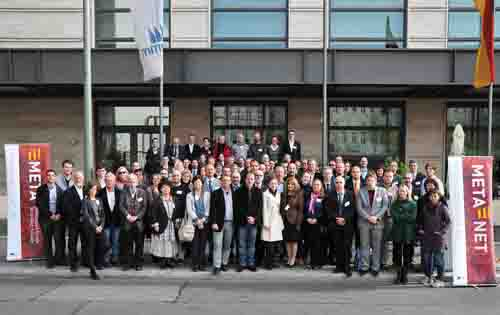
\includegraphics[width=\textwidth]{../_media/meta-net_team.jpg}
  \caption{SERBIAN --- \textcolor{grey1}{About 100 language technology experts -- representatives of the countries and languages represented in META-NET -- discussed and finalised the key results and messages of the White Paper Series at a META-NET meeting in Berlin, Germany, on October 21/22, 2011.}}
  \medskip
  \colorrule{grey3}{\textwidth}{1.5pt}
\end{figure*}


\bsection[МЕТА-НЕТ серија белих књига -- The META-NET White Paper Series]{МЕТА-НЕТ серија белих књига --- The META-NET White Paper Series}
\label{whitepaperseries}

\renewcommand{\arraystretch}{1}
\begin{center}
\begin{tabulary}{170mm}{LLL} \toprule
  баскијски & Basque & euskara\\
  бугарски & Bulgarian & български \\
  галицијски & Galician & galego\\
  грчки & Greek & ελληνικά \\
  дански & Danish & dansk\\
  енглески & English & English\\
  естонски & Estonian & eesti\\
  ирски & Irish & Gaeilge\\
  исландски & Icelandic & íslenska \\
  италијански & Italian & italiano\\
  каталонски & Catalan & català \\
  летонски & Latvian &  latviešu valoda\\
  литвански & Lithuanian & lietuvių kalba\\
  мађарски & Hungarian & magyar\\
  малтешки & Maltese & Malti\\
  немачки & German & Deutsch\\
  норвешки бокмал & Norwegian Bokmål & bokmål \\
  норвешки нинорск & Norwegian Nynorsk & nynorsk\\
  пољски & Polish & polski\\
  португалски & Portuguese & português\\
  румунски & Romanian & română\\
  словачки & Slovak & slovenčina\\
  словеначки & Slovene & slovenščina\\
  српски & Serbian & српски \\
  фински & Finnish & suomi\\
  француски & French & français\\
  холандски & Dutch & Nederlands\\
  хрватски & Croatian & hrvatski\\
  чешки & Czech & čeština\\
 шведски & Swedish & svenska\\
 шпански & Spanish & español\\
   \addlinespace \bottomrule
\end{tabulary}
\end{center}
